\documentclass[a4paper]{article}
\usepackage{a4wide,amssymb,epsfig,latexsym,multicol,array,hhline,fancyhdr}
\usepackage{vntex}
\usepackage{amsmath}
\usepackage{lastpage}
\usepackage[lined,boxed,commentsnumbered]{algorithm2e}
\usepackage{enumerate}
\usepackage{color}
\usepackage{graphicx}							% Standard graphics package
\usepackage{array}
\usepackage{tabularx, caption}
\usepackage{multirow}
\usepackage{multicol}
\usepackage{rotating}
\usepackage{graphics}
\usepackage{geometry}
\usepackage{setspace}
\usepackage{epsfig}
\usepackage{tikz}
\usetikzlibrary{arrows,snakes,backgrounds}
\usepackage{hyperref}
\usepackage{indentfirst}
\usepackage{longtable}
\hypersetup{urlcolor=blue,linkcolor=black,citecolor=black,colorlinks=true} 
%\usepackage{pstcol} 								% PSTricks with the standard color package

\newtheorem{theorem}{{\bf Theorem}}
\newtheorem{property}{{\bf Property}}
\newtheorem{proposition}{{\bf Proposition}}
\newtheorem{corollary}[proposition]{{\bf Corollary}}
\newtheorem{lemma}[proposition]{{\bf Lemma}}

\AtBeginDocument{\renewcommand*\contentsname{Mục lục}}
\AtBeginDocument{\renewcommand*\refname{Tài liệu tham khảo}}
%\usepackage{fancyhdr}
\setlength{\headheight}{40pt}
\pagestyle{fancy}
\fancyhead{} % clear all header fields
\fancyhead[L]{
	\begin{tabular}{rl}
		\begin{picture}(25,15)(0,0)
			\put(0,-8){
\includegraphics[width=8mm, height=8mm]{hcmut.png}}
			%\put(0,-8){\epsfig{width=10mm,figure=hcmut.eps}}
		\end{picture}&
		%
\includegraphics[width=8mm, height=8mm]{hcmut.png} & %
		\begin{tabular}{l}
			\textbf{\bf \ttfamily Trường Đại học Bách khoa Thành phố Hồ Chí Minh}\\
			\textbf{\bf \ttfamily Khoa Khoa học và Kỹ thuật Máy tính}
		\end{tabular} 	
	\end{tabular}
}
\fancyhead[R]{
	\begin{tabular}{l}
		\tiny \bf \\
		\tiny \bf 
\end{tabular}  }
\fancyfoot{} % clear all footer fields
\fancyfoot[L]{\scriptsize \ttfamily Bài tập lớn Công nghệ Phần mềm - Học kỳ 2023 - 2024}
\fancyfoot[R]{\scriptsize \ttfamily Trang {\thepage}/\pageref{LastPage}}
\renewcommand{\headrulewidth}{0.3pt}
\renewcommand{\footrulewidth}{0.3pt}


%%%
\setcounter{secnumdepth}{4}
\setcounter{tocdepth}{3}
\makeatletter
\newcounter {subsubsubsection}[subsubsection]
\renewcommand\thesubsubsubsection{\thesubsubsection .\@alph\c@subsubsubsection}
\newcommand\subsubsubsection{\@startsection{subsubsubsection}{4}{\z@}%
	{-3.25ex\@plus -1ex \@minus -.2ex}%
	{1.5ex \@plus .2ex}%
	{\normalfont\normalsize\bfseries}}
\newcommand*\l@subsubsubsection{\@dottedtocline{3}{10.0em}{4.1em}}
\newcommand*{\subsubsubsectionmark}[1]{}
\makeatother


\begin{document}
	
	\begin{titlepage}
		\begin{center}
			ĐẠI HỌC QUỐC GIA THÀNH PHỐ HỒ CHÍ MINH \\
			TRƯỜNG ĐẠI HỌC BÁCH KHOA \\
			KHOA KHOA HỌC \& KỸ THUẬT MÁY TÍNH
		\end{center}
		
		\vspace{1cm}
		
		\begin{figure}[h!]
			\begin{center}
				
\includegraphics[width=3cm]{hcmut.png}
			\end{center}
		\end{figure}
		
		\vspace{1cm}
		
		
		\begin{center}
			\begin{tabular}{c}
				\multicolumn{1}{l}{\textbf{{\Large CÔNG NGHỆ PHẦN MỀM (CO3001)}}}\\
				~~\\
				\hline
				\\
				\multicolumn{1}{l}{\textbf{{\Large Bài tập lớn}}}\\
				\\
				\textbf{{\Huge HCMUT\_SSPS}}\\
				\\
				\hline
			\end{tabular}
		\end{center}
		
		\vspace{3cm}
		
		\begin{table}[h]
			\begin{tabular}{rrl}
				\hspace{5 cm} & Giảng viên hướng dẫn: & Lê Đình Thuận\\
				& Sinh viên thực hiện: & Hà Thùy Dương - 2110103 \\
				& & Lê Quang Hiển - 2113376\\
 & & Bùi Quang Hưng - 2111392 \\
 & & Võ Tấn Tài - 2110516 \\
 & & Nguyễn Văn Ngọc Quang - 2114511\\
			\end{tabular}
		\end{table}
		
		\begin{center}
			{\footnotesize Thành phố Hồ Chí Minh, Tháng 9/2023}
		\end{center}
	\end{titlepage}
	
	
	%\thispagestyle{empty}
	
	\newpage
	\tableofcontents
	\newpage
	
	
	%%%%%%%%%%%%%%%%%%%%%%%%%%%%%%%%%
	\section{Task 1: Requirement elicitation}
	\subsection{Task 1.1}
    \subsubsection{Describe the domain context of a smart printing service for students at HCMUT}
    Tác dụng của máy in trong thời đại công nghệ số là điều mà không ai có thể phủ nhận, mang đến tính ứng dụng cao, hiệu quả kinh tế lớn. Hiện nay, hầu hết các trường học đều trang bị hệ thống máy in, giải quyết nhanh chống việc in ấn tài liệu, nâng cao hiệu quả và chất lượng học tập của các học sinh, sinh viên.\\
    
    Máy in ngày nay được tích hợp rất nhiều chức năng, thao tác in ấn đơn giản dễ tiếp cận người dùng. Tuy nhiên, khi số lượng người dùng càng tăng thì việc quản lí hệ thống máy in này càng trở nên khó khăn và dễ dàng vượt ra khỏi tầm kiêm soát. Các hoạt động như in sai tài liệu, quên lấy bản in từ máy in, vô ý in nhiều lần một tài liệu cụ thể, in tài liệu một mặt thay vì hai mặt… là những đặc điểm của lãng phí in ấn trong nội bộ tổ chức. Do đó, việc triển khai hệ thống quản lí in ấn (HCMUT\_SSPS) phải được đề cao hơn bao giờ hết, giúp giảm những chi phí không đáng có, xử lý yêu cầu một cách tự động nhằm hướng tới một tương lai in ấn xanh hơn.\\

    Dịch vụ in ấn thông minh dành cho sinh viên (HCMUT\_SSPS) trong bài tập lớn này có các đặc điểm chính sau:
    \begin{itemize}
    \item Hệ thống quản lí chuỗi các máy in trong khuôn viên trường.
    \item Quy mô vừa và nhỏ, đáp ứng đủ các tính năng cơ bản của việc in ấn tài liệu.
    \item Đối tượng người dùng là sinh viên trường Đại học Bách Khoa.
    \item Sinh viên sẽ được nhà trường cung cấp một số lượng trang A4 mặc định để in trong mỗi học kì.
    \item Hỗ trợ tính năng mua thêm trang in (Buy Printing Pages) và thanh toán trực tuyến.
    \end{itemize}

    Từ những phân tích trên, HCMUT\_SSPS cần được xây dựng đơn giản, dễ sử dụng, thân thiện với người dùng. Hơn nữa, chúng ta cần tập trung vào vấn đề bảo mật thông tin vì dịch vụ này có cung cấp chức năng thanh toán điện tử.
    \subsubsection{Who are relevant stakeholders? What are their current needs?}
    Với nhu cầu sử dụng máy in cao của sinh viên, hệ thống HCMUT\_SPSS sẽ có những cổ đông (stakeholders) có hứng thú với hệ thống, bao gồm:
    \begin{itemize}
        \item Sinh viên trường Đại học Bách Khoa: Nhu cầu in tài liệu; tải (upload) tài liệu lên hệ thống; chọn địa điểm, thời gian, máy in; xác định các thuộc tính in theo nhu cầu; xem lịch sử in ấn; xem số dư tài khoản; nạp tiền và thanh toán cho việc in hoặc mua thêm giấy in.
        \item Student Printing Service Officer (SPSO): Quản lý và kiểm soát máy in (thêm hoặc xóa máy in/bật/tắt); có khả năng thay đổi cấu hình của dịch vụ (số trang in cấp sẵn/giá thành của giấy in/định dạng file cho phép được in); xem lịch sử in ấn của từng sinh viên hoặc máy in; xem báo cáo theo tháng hoặc năm của từng sinh viên hoặc máy in.
        \item Ban quản trị thuộc trường Đại học Bách Khoa: Tích hợp dịch vụ HCMUT\_SSO nhằm bảo đảm tính bảo mật; quản lý sinh viên.
        \item Bộ phận kĩ thuật: Cung cấp hệ thống HCMUT\_SPSS, bảo đảm tính bảo mật, bảo trì, nâng cấp hệ thống để phù hợp với quy mô và nhu cầu sử dụng.
    \end{itemize}
    
    Mỗi cổ đông đều có những nhu cầu như sau:
    \begin{itemize}
        \item Sinh viên trường Đại học Bách Khoa \text{--} là đối tượng chính của hệ thống HCMUT\_SPSS:
        \begin{itemize}
            \item Có thể xác định vị trí máy in thuận tiện, thuận tiện hơn cho sinh viên trong việc di chuyển.
            \item Có thể tải tài liệu lên hệ thống, tiết kiệm thời gian chờ đợi, tăng sự tiện lợi.
            \item Có khả năng xem số trang in hiện có, số dư tài khoản, nhằm tăng khả năng quản lý chi tiêu cho sinh viên, đồng thời tiện lợi cho việc nạp tiền và thanh toán.
            \item Có tính năng giao tiếp nhằm hỗ trợ sinh viên khi dịch vụ gặp những trục trặc.
        \end{itemize}
        \item Student Printing Service Officer (SPSO) \text{--} Ban quản trị của hệ thống HCMUT\_SPSS:
        \begin{itemize}
            \item Có khả năng quản lý các máy in, thêm hoặc loại bỏ các máy in trong hệ thống, đồng thời cho phép máy in nào hoạt động; cập nhật phần mềm/phần cứng nhằm thuận tiện cho việc quản lý, bảo trì.
            \item Có thể thay đổi cấu hình in như: cỡ giấy tiêu chuẩn, loại file, cỡ chữ, font chữ, giá thành, số trang mặc định để phù hợp với thị hiếu của sinh viên.
            \item Xem được lịch sử in ấn của từng máy in và sinh viên, nhằm lấy được các thông tin cần thiết về những máy in hay tài liệu phổ biến để có phương pháp bố trí hiệu quả hơn.
            \item Có tính năng hỗ trợ sinh viên khi sinh viên gặp trục trặc với hệ thống.
        \end{itemize}
        \item Ban quản trị thuộc trường Đại học Bách Khoa \text{--} là những người điều hành trường Đại học Bách Khoa:
            \begin{itemize}
                \item Tích hợp dịch vụ HCMUT\_SSO, vừa thuận tiện cho việc quản lý, vừa thuận tiện cho nhu cầu bảo mật.
                \item Xem được các báo cáo hàng tháng/hàng năm của từng máy in hoặc cả một hệ thống để có thể kiểm soát dịch vụ, cải thiện, nâng cao chất lượng dịch vụ.
            \end{itemize}
            \item Bộ phận kĩ thuật \text{--} là bên cung cấp, duy trì dịch vụ hoạt động một cách hiệu quả:
            \begin{itemize}
                \item Bộ phận kĩ thuật cần những yêu cầu minh bạch nhằm phát triển hệ thống một cách chính xác, hiệu quả.
            \end{itemize}
    \end{itemize}
    \subsubsection{In your opinion, what benefits HCMUT-SSPS will be for each stakeholder?}   
	Khi hệ thống HCMUT\_SPSS được triển khai, nó sẽ mang lại nhiều lợi ích cho các stakeholders liên quan tới dự án. Những stakesholders được hưởng nhiều lợi ích nhất từ phần mềm SSPS là những nhân tố chính mà phần mềm này được thiết kế để phục vụ đó là 2 bên nhà trường và sinh viên.
    \begin{itemize}
        \item Sinh viên trường Đại học Bách khoa
            \begin{itemize}
                \item Hệ thống hỗ trợ sinh viên trong việc in ấn tài liệu học tập một cách tiện lợi, linh động hơn.
                \item Thuận tiện trong việc thanh toán tài liệu đã được in ấn thông qua hệ thống BKPay.
                \item Kiểm tra được lịch sử in tài liệu của cá nhân.
            \end{itemize}
        \item Ban quản trị trường Đại học Bách khoa
            \begin{itemize}
                \item Cung cấp cho sinh viên một tiện ích mới nhằm nâng cao chất lượng học tập.
                \item Cải thiện cơ sở vật chất, nâng cao chất lượng môi trường giáo dục của trường Đại học Bách khoa.
                \item Nhờ chức năng thu thập và báo cáo dữ liệu. Nhà trường có thể theo dõi thói quen, hành vi in tài liệu của sinh viên một cách tiện lợi hơn, nhờ đó chất lượng của dịch vụ HCMUT\_SSPS không ngừng được cải thiện.
            \end{itemize}
    \end{itemize}
        \subsection{Task 1.2}
    \subsubsection{Describe all functional requirements that can be inferred from the project description.}
        \textbf{Sinh viên:}
            \begin{itemize}
                \item Sinh viên có thể tải tệp lên hệ thống, chọn máy in và chỉ định các thuộc tính in như khổ giấy, trang, in một mặt hoặc hai mặt, số bản được in,...
                \item Sinh viên có thể xem lịch sử in trong một khoảng thời gian kèm theo bản tóm tắt số trang đã in cho từng kích thước trang.
                \item Sinh viên có thể mua thêm số lượng giấy để in nhiều hơn số tờ mặc định được cấp sẵn.
                \item Sinh viên thanh toán trả trước qua một số hệ thống thanh toán trực tuyến như BKPay.
            \end{itemize}
            
        \textbf{Quản lý dịch vụ in (SPSO):}
            \begin{itemize}
                \item SPSO có quyền thêm máy in vào hệ thống.
                \item SPSO có quyền kích hoạt một máy in trong hệ thống.
                \item SPSO có quyền dừng hoạt động một máy in trong hệ thống.
                \item SPSO có thể giới hạn và tùy chỉnh các định dạng tệp mà sinh viên có thể tải lên hệ thống.
                \item SPSO có thể quản lý cấu hình của hệ thống như thay đổi số trang mặc định, thời điểm mà hệ thống sẽ cung cấp số trang mặc định cho tất cả sinh viên.
                \item SPSO có thể xem lịch sử in ấn của tất cả sinh viên và tất cả các máy in.
            \end{itemize}
            
        \textbf{Hệ thống:}
            \begin{itemize}
                \item Tất cả người dùng phải được xác thực bằng dịch vụ xác thực HCMUT\_SSO trước khi sử dụng hệ thống.
                \item Giao diện web và mobile được hỗ trợ.
                \item Hệ thống ghi lại các thao tác in ấn của tất cả sinh viên, bao gồm mã sinh viên, mã máy in, tập tin tên, thời gian bắt đầu và kết thúc in, số trang cho mỗi khổ giấy.
                \item Các báo cáo về việc sử dụng hệ thống in được tạo tự động vào cuối mỗi tháng, mỗi năm và được lưu trữ trong hệ thống và SPSO có thể xem bất cứ lúc nào.
                \item Trong mỗi học kỳ, trường sẽ cấp cho mỗi sinh viên một số lượng giấy A4 mặc định để in ấn.
                \item Một trang giấy A3 có thành tiền bằng hai trang giấy A4.
                \item Hệ thống lưu trữ thông tin của một máy in bao gồm ID, nhãn hiệu hoặc hãng sản xuất, mẫu mã, mô tả ngắn về máy in, vị trí máy in cụ thể là tên cơ sở của trường, tên tòa nhà và số phòng.
            \end{itemize}
    \subsubsection{Describe all non-functional requirements that can be inferred from the project description.}
	\textbf{Yêu cầu về hiệu suất:}
            \begin{itemize}
                \item Các trang của ứng dụng web phải được tải trong thời gian không quá 3 giây trên kết nối internet với tốc độ truy cập trung bình.
                \item Tốc độ phản hồi của hệ thống với các thao tác của người dùng diễn ra không quá 1 giây.
                \item Hệ thống phải hỗ trợ ít nhất 100 người dùng đồng thời mà không gây ra giảm hiệu suất đáng kể (dưới 10\%).
                \item Ứng dụng web không được sử dụng nhiều hơn 300MB RAM trên thiết bị người dùng.
            \end{itemize}
    
        \textbf{Yêu cầu về bảo mật và an ninh:}
            \begin{itemize}
                \item Đảm bảo rằng tất cả người dùng đều phải xác thực thông qua dịch vụ xác thực HCMUT\_SSO trước khi sử dụng hệ thống.
                \item Tại cùng 1 thời điểm, 1 tài khoản chỉ được đăng nhập trên 1 thiết bị.
                \item Khóa tài khoản người dùng sau 5 lần đăng nhập sai mật khẩu liên tiếp.
                \item Đảm bảo rằng người dùng chỉ có quyền truy cập và thực hiện các tác vụ phù hợp với vai trò của họ.
                \item Triển khai biện pháp bảo vệ để ngăn chặn tấn công DDoS và đảm bảo sự ổn định của hệ thống.
                \item Phần mềm phải tuân thủ luật pháp của Việt Nam về an toàn thông tin mạng.
            \end{itemize}
            
        \textbf{Yêu cầu về độ tin cậy:}
            \begin{itemize}
                \item Hệ thống phải sẵn sàng và hoạt động một cách ổn định trong khoảng thời gian từ 6 giờ đến 22 giờ hằng ngày.
                \item Đảm bảo rằng có hệ thống sao lưu định kỳ và khả năng phục hồi dữ liệu nhanh chóng trong trường hợp sự cố hoặc mất dữ liệu.
                \item Tỉ lệ xảy ra lỗi không quá 0.5\%.
            \end{itemize}

        \textbf{Yêu cầu về khả năng sử dụng:}
                \begin{itemize}
                \item Giao diện người dùng của ứng dụng web phải được thiết kế một cách trực quan và người sử dụng có thể làm quen sau không quá 10 phút.
                \item Đảm bảo ứng dụng web có thể hoạt động hiệu quả trên nhiều trình duyệt web phổ biến (Chrome, Firefox, Safari, Edge) và phải đáp ứng trên các loại thiết bị (máy tính xách tay, điện thoại thông minh, máy tính bảng).
                \item Hệ thống phải hỗ trợ các hệ điều hành phổ biến (iOS, Android, Windows).
                \item Hệ thống cần hỗ trợ ít nhất 2 ngôn ngữ (Anh và Việt) và cung cấp lựa chọn để người dùng có thể chọn ngôn ngữ phù hợp với họ.
                \item Đảm bảo hệ thống có thể làm việc với nhiều định dạng và thuộc tính file khác nhau
                \end{itemize} 
                
        \textbf{Yêu cầu về khả năng quản lí:}
                \begin{itemize}
                \item Hệ thống phải kết nối với hệ thống thanh toán trực tuyến (ví dụ: BKPay) và kiểm tra thanh toán thành công trước khi cho phép in.
                \item Đảm bảo rằng SPSO có thể dễ dàng thêm, bật/tắt máy in, và chỉnh sửa thông tin máy in.
                \item Đảm bảo rằng SPSO có khả năng thay đổi cấu hình hệ thống như số trang mặc định, ngày mà hệ thống cung cấp số trang mặc định cho sinh viên, và danh sách các định dạng tệp cho phép.
                \end{itemize}
                
        \textbf{Yêu cầu về khả năng bảo trì:}
                \begin{itemize}
                \item Thực hiện kiểm tra định kỳ mỗi 3 tháng để đảm bảo rằng hệ thống đang hoạt động đúng cách và tuân thủ các tiêu chuẩn bảo mật và hiệu suất.
                \item Thời gian bảo trì nâng cấp, sửa lỗi hoặc cập nhật hệ thống không kéo dài quá 1 giờ.
                \end{itemize}
                
        \textbf{Yêu cầu về khả năng mở rộng:} Hệ thống có thể mở rộng số lượng máy in, số lượng người truy cập cùng lúc trong hệ thống mà không gây ra giảm hiệu suất đáng kể (dưới 10\%) trong tương lai lên gấp đôi. \\
        
        \textbf{Yêu cầu về tính toàn vẹn, chính xác:} Kết quả tính toán giá tiền của đơn hàng luôn chính xác 100\%.  
        \newpage
    \subsection{Task 1.3}
    \subsubsection{Draw a use-case diagram for the whole system}
    \begin{center}
    \begin{figure}[htp]
    \begin{center}
     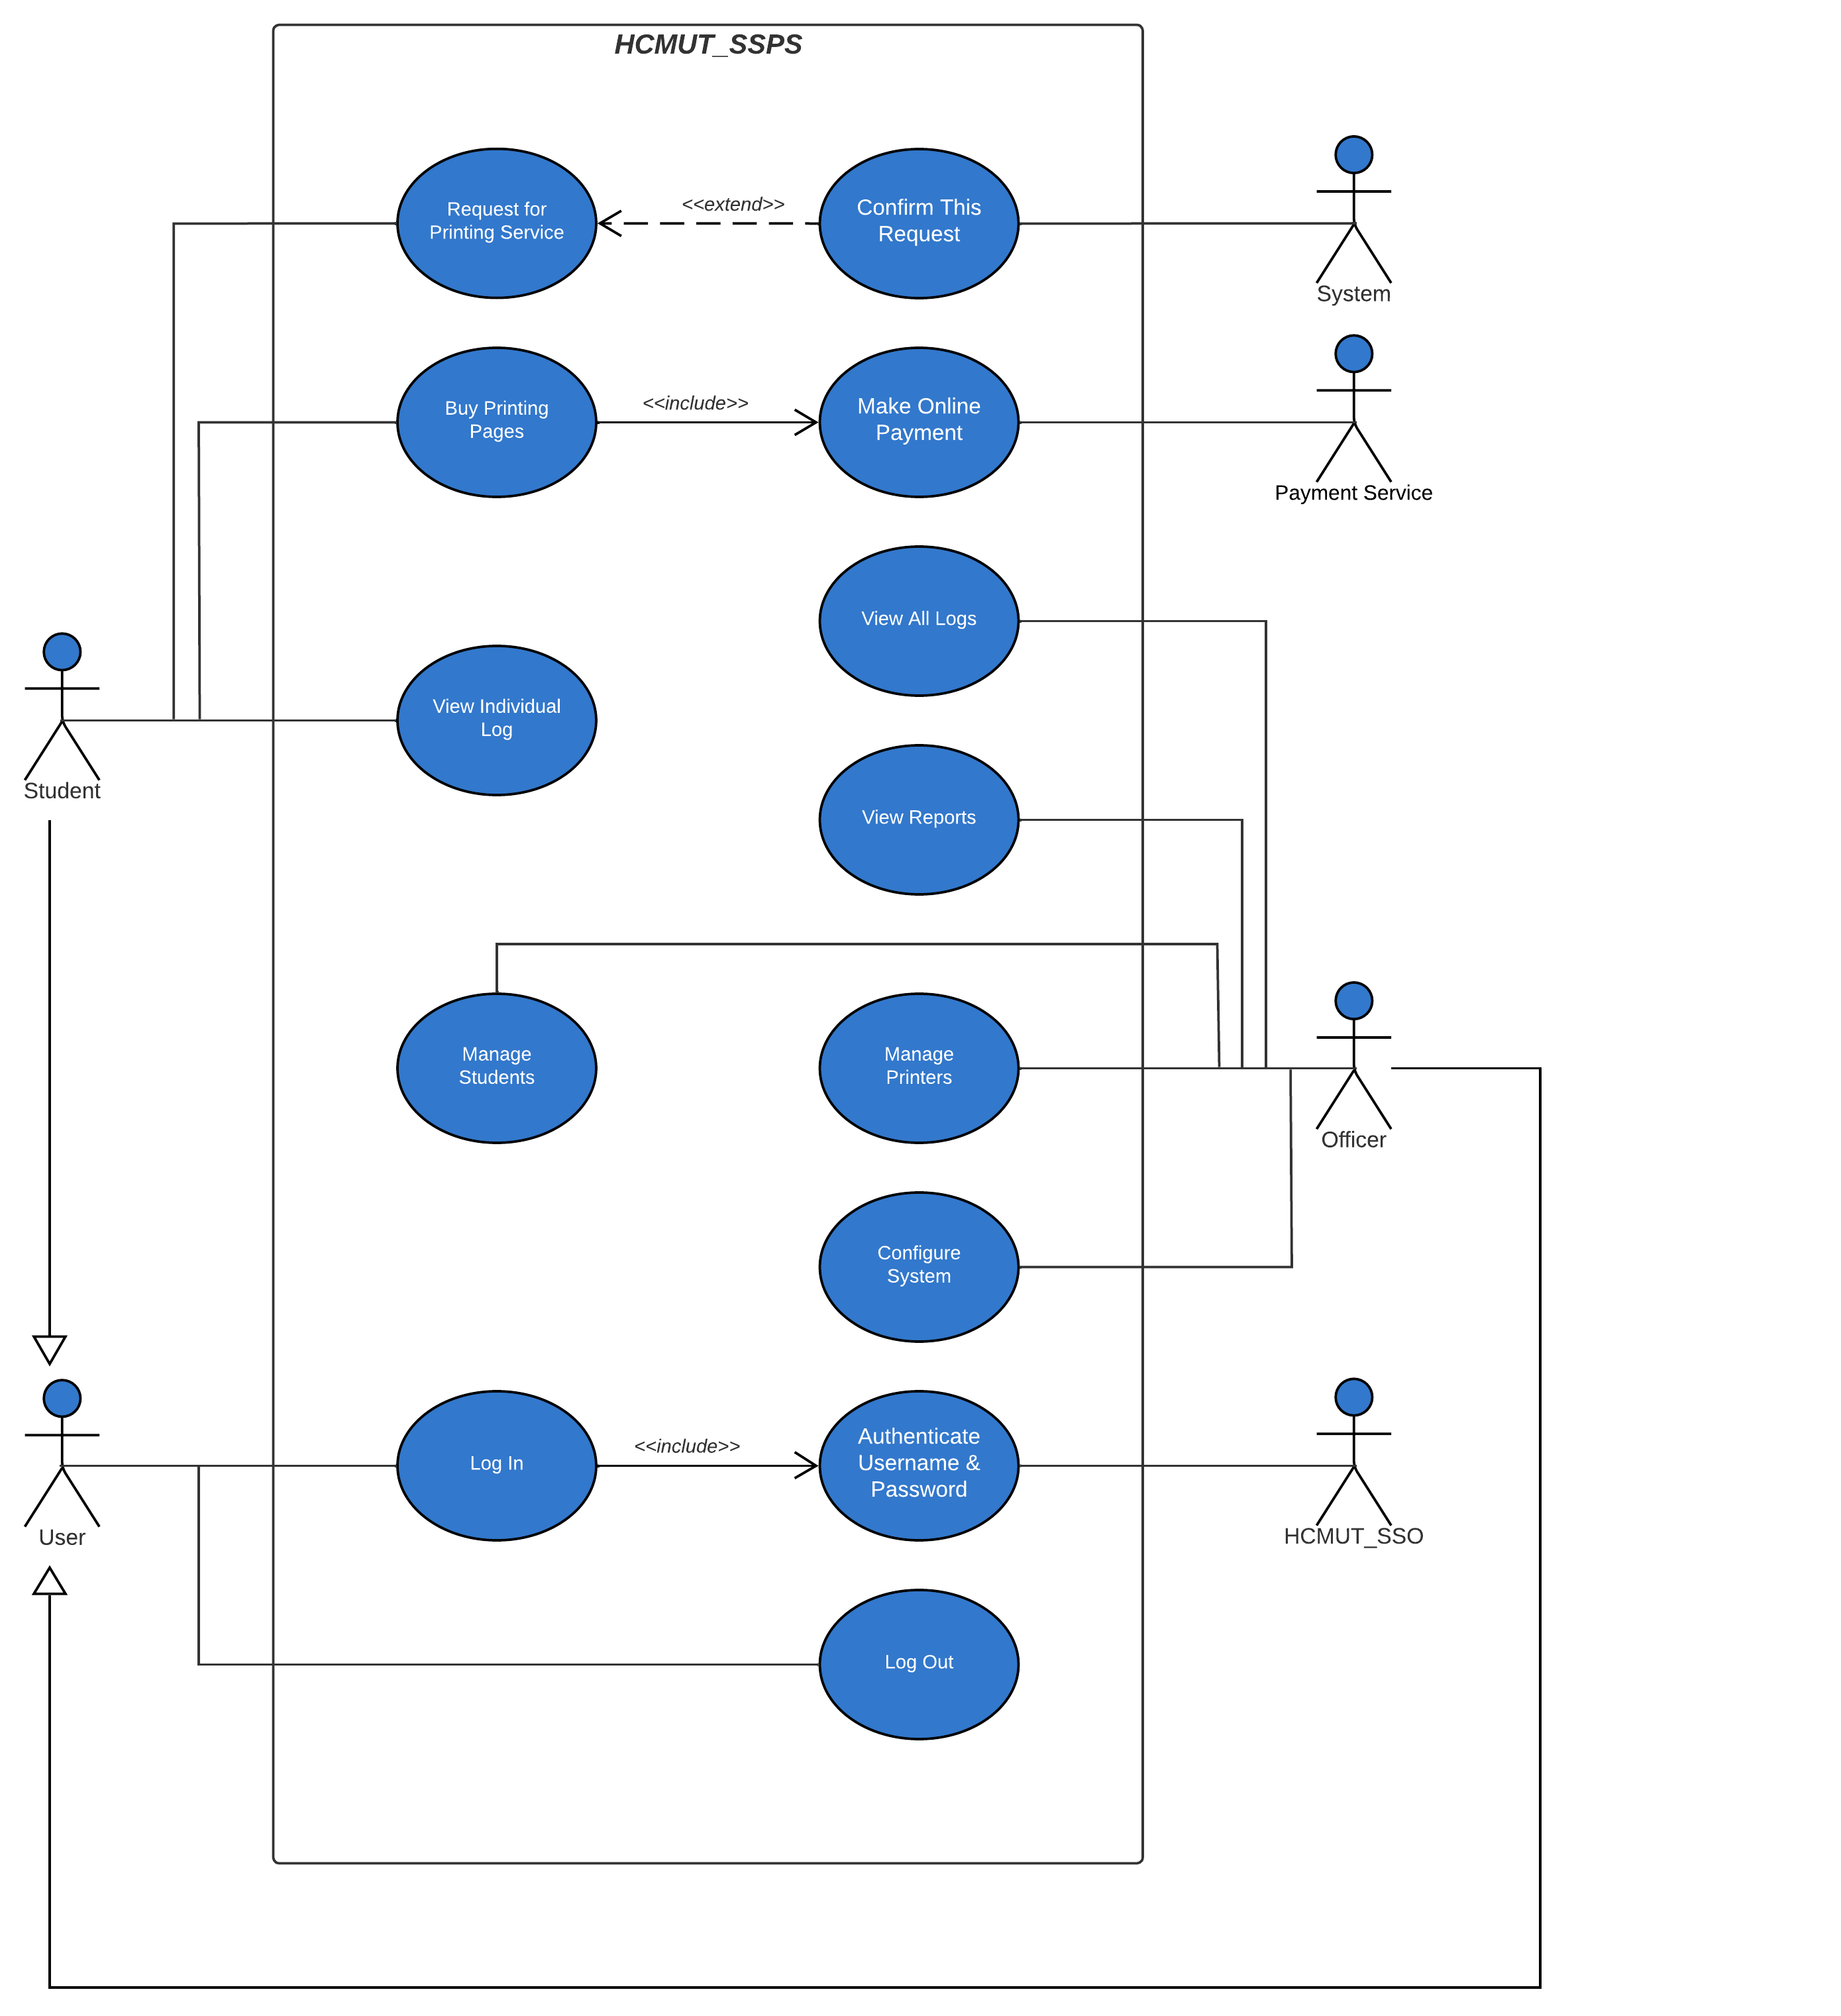
\includegraphics[scale=.62]{images/Task1/wholeSystem.png}
    \end{center}
    \label{refhinh1}
    \end{figure}
    \end{center}

    \newpage
    \subsubsection{Choose an important module and draw its use-case diagram, as well as describe the use-case using a table format}

    \begin{enumerate}[a)]
    \item {\textbf{Request for Printing Service}}
    \begin{center}
    \begin{figure}[htp]
    \begin{center}
     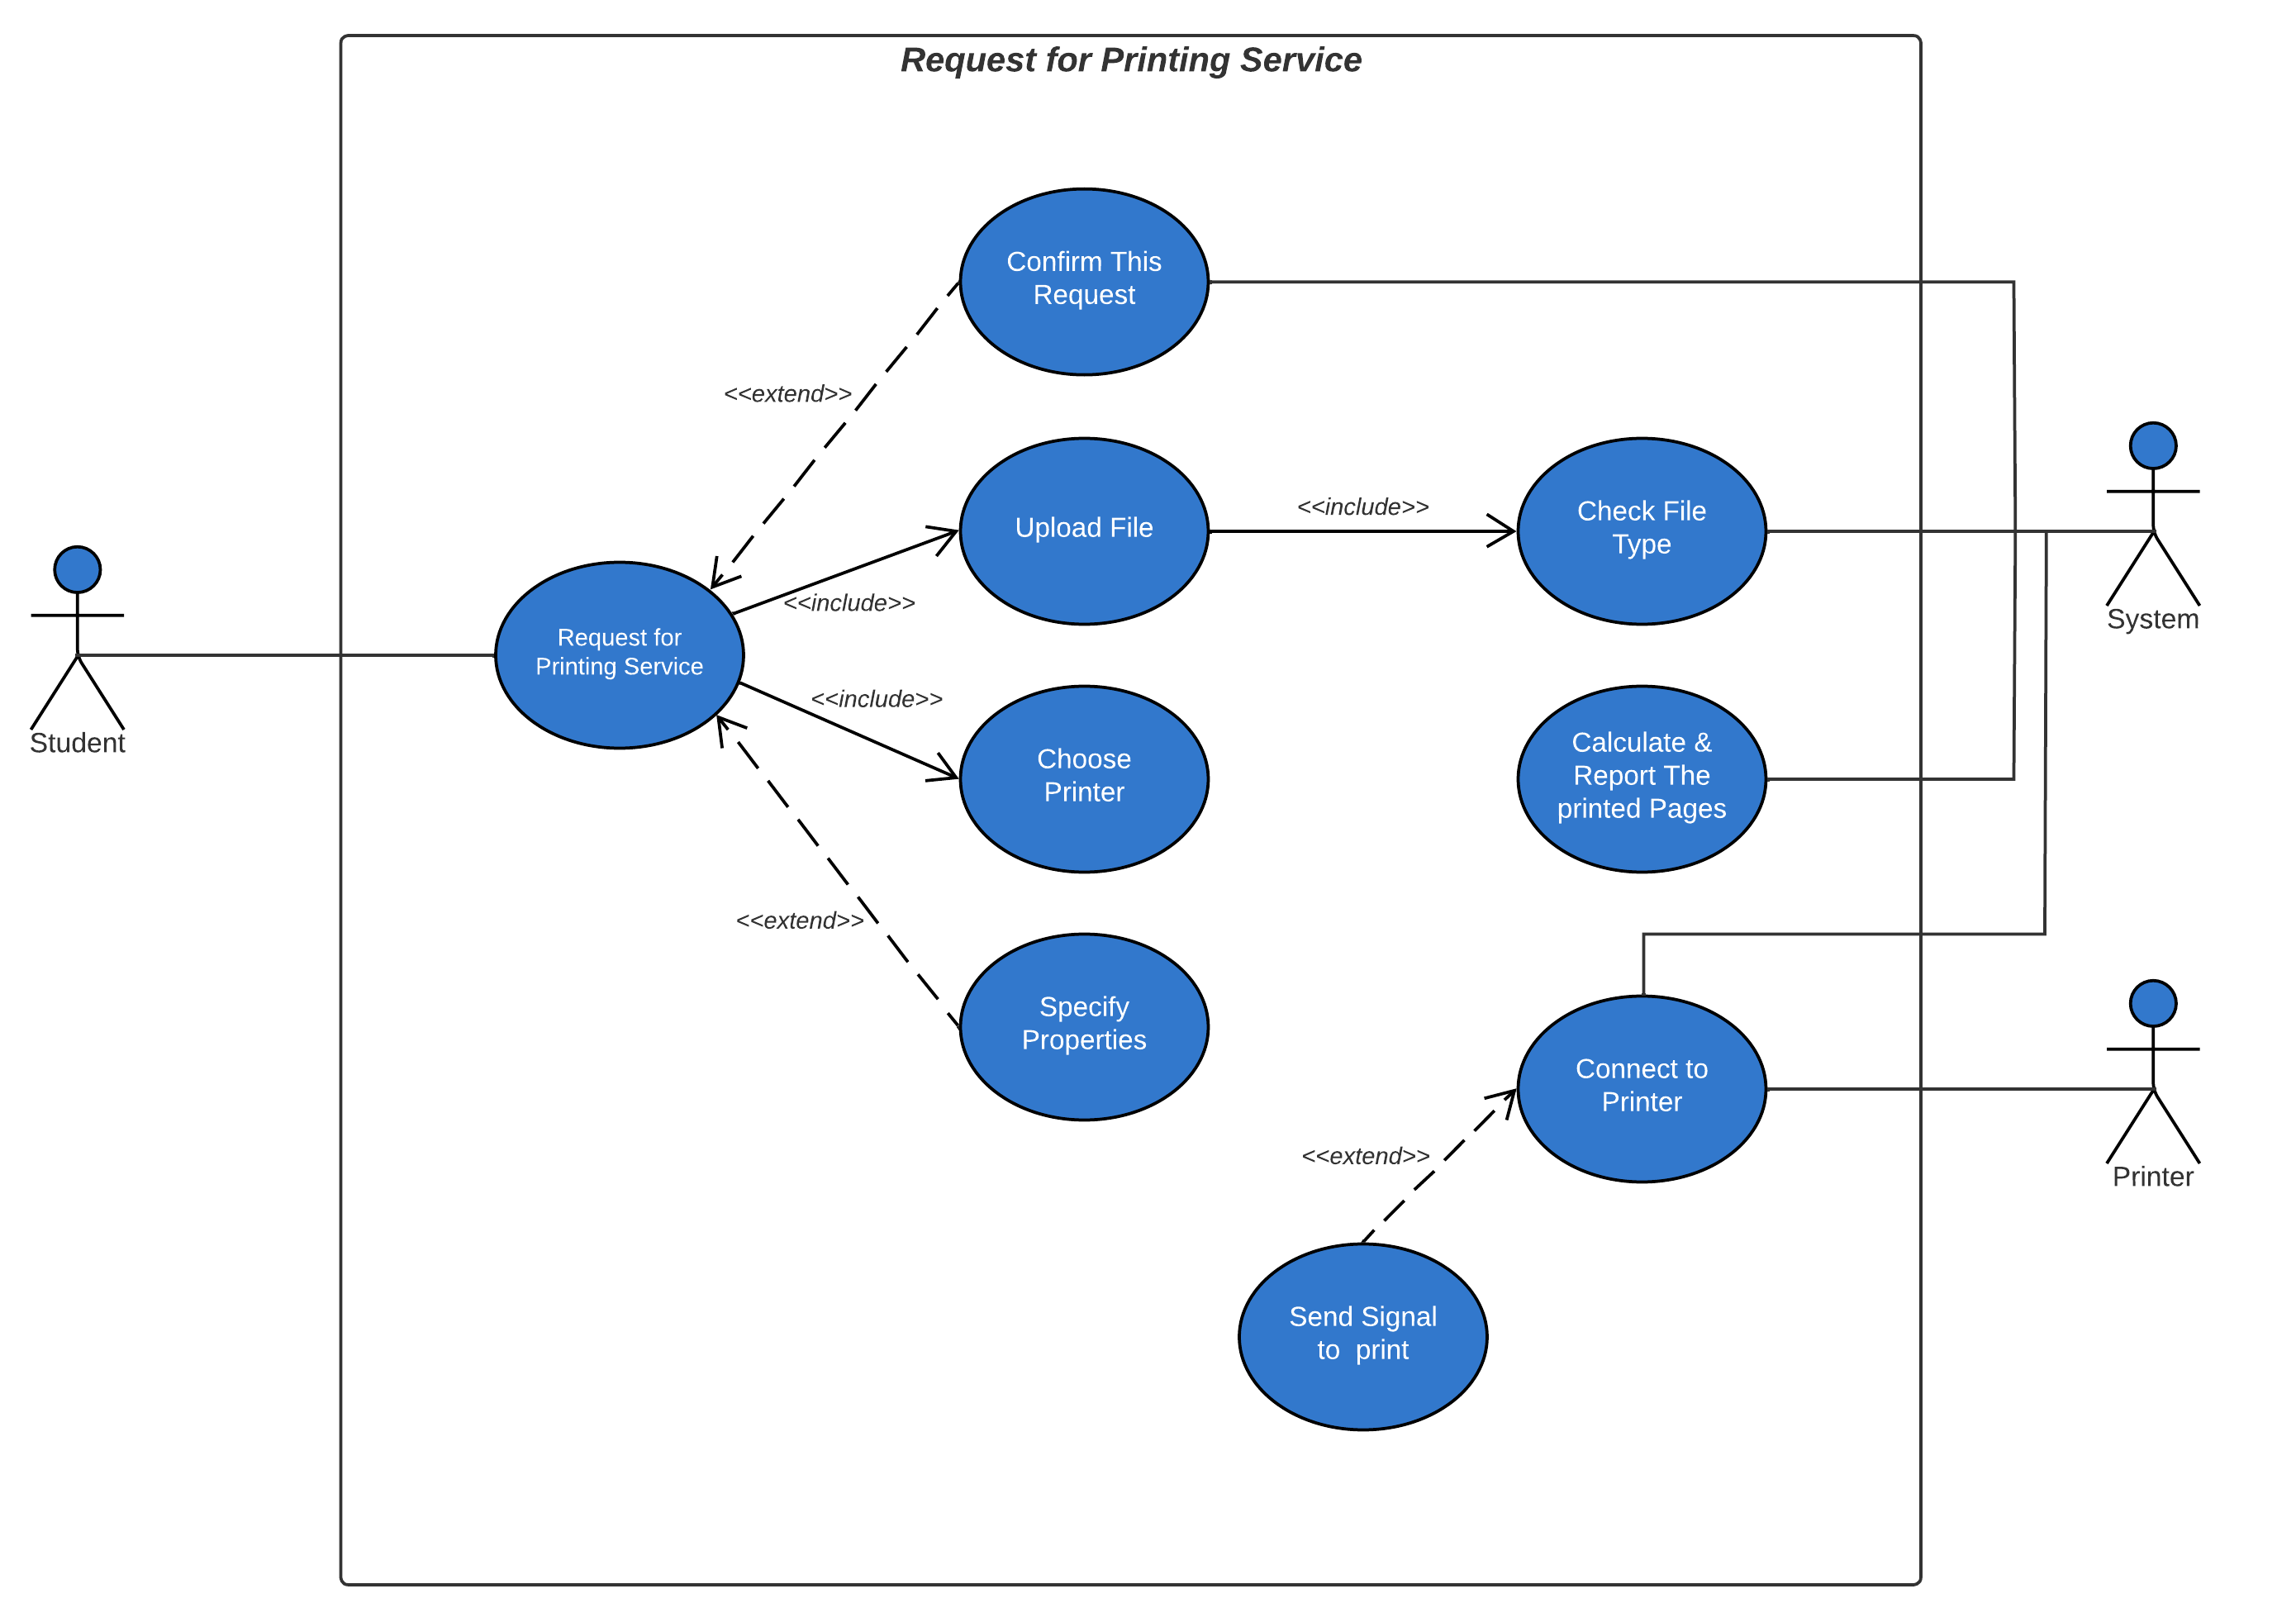
\includegraphics[scale=.62]{images/Task1/requestForPrintingService.png}
    \end{center}
    \label{refhinh1}
    \end{figure}
    \end{center}

    \begin{longtable}{|l|p{10cm}|}
        \hline
        \endhead
        \hline
        \endfoot
        Use-case Name & \textbf{Request for Printing Service}\\
        \hline
        Actors & Sinh viên.\\
        \hline
        Description & Sinh viên sử dụng chức năng này để tiến hành thực hiện in tài liệu thông qua hệ thống máy in của nhà trường.\\
        \hline
        Trigger & Sinh viên nhấn vào nút "In tài liệu".\\
        \hline
        Pre-conditions & Sinh viên đăng nhập vào hệ thống thành công.\\
        \hline
        Post-conditions & None.\\
        \hline
        Basic Flow & 1. Sinh viên chọn mục "Dịch vụ".\\
        & 2. Sinh viên chọn "In tài liệu".\\
        & 3. Hệ thống hiển thị các trường thông tin mà sinh viên cần phải cung cấp.\\
        & 4. Sinh viên tải tài liệu cần in lên hệ thống.\\
        & 5. Hệ thống kiểm tra loại tài liệu sinh viên cung cấp có thuộc một trong các loại được hệ thống cho phép hay không.\\
        & 6. Sinh viên chọn máy in mà mình muốn kết nối để sử dụng.\\
        & 7. Các thuộc tính in sẽ có giá trị mặc định. Tuy nhiên, sinh viên có thể điều chỉnh lại các thuộc tính in này cho phù hợp với nhu cầu.\\
        & 8. Sinh viên nhấn vào nút "Hoàn tất" để hoàn thành các tuỳ chọn.\\
        & 9. Hệ thống hiển thị tổng quát các thông tin mà sinh viên đã cung cấp.\\
        & 10. Sinh viên nhấn vào nút "Tiến hành in" để xác nhận gửi yêu cầu in tài liệu đến hệ thống.\\
        & 11. Hệ thống tiếp nhận và xử lý yêu cầu. Hệ thống sẽ tính toán số lượng trang in miễn phí còn lại của mỗi sinh viên và thông báo số lượng trang in mà sinh viên cần mua thêm.\\ 
        & 12. Hệ thống thông báo dịch vụ in được xác nhận thành công và tiến hành in tài liệu cho sinh viên.\\

        \hline
        Alternative Flow & Alternative 1: Sau bước 4,  nếu tài liệu được tải lên không hợp lệ:\\
        & \hspace{1em} 4.1. Hệ thống hiện thông báo "Tài liệu này có định dạng không hợp lệ. Vui lòng chọn một tài liệu khác!".\\
        & \hspace{1em} 4.2. Sinh viên chọn "Đồng ý" để quay lại bước 4 trong \textit{Basic Flow} và tải lên lại một tài liệu khác.\\
        &\\
        & Alternative 2: Sau bước 8, nếu có ít nhất một trong các trường thông tin bị để trống:\\
        & \hspace{1em} 8.1. Hệ thống thông báo việc gửi yêu cầu in của sinh viên thất bại và chỉ ra những trường thông tin còn trống đó.\\
        & \hspace{1em} 8.2. Sinh viên cung cấp đầy đủ các thông tin mà hệ thống yêu cầu và quay lại bước 7 trong \textit{Basic Flow}.\\
         &\\
        & Alternative 3: Sau bước 9, nếu một số thông tin về dịch vụ cần được thay đổi:\\
        & \hspace{1em} 9.1. Sinh viên chọn "Quay lại" để quay về bước 4 trong \textit{Basic Flow} để điều chỉnh lại các thông tin cho phù hợp.\\
        &\\
        & Alternative 4: Sau bước 11, nếu số lượng trang in cần cho yêu cầu in hiện tại vượt quá số lượng trang in miễn phí còn lại của sinh viên:\\
        & \hspace{1em} 11.1. Sinh viên chọn "Mua thêm" để sử dụng tính năng mua thêm trang in (Buy Printing Pages) và tiếp tục bước 12 trong \textit{Basic Flow}.\\
        \hline
        Exception Flow & Exception 1: Sau bước 4.1, sinh viên có thể chọn "Thoát" để huỷ dịch vụ in và trở về trang chủ.\\
        &\\
        & Exception 2: Sau bước 8.1, sinh viên có thể chọn "Thoát" để huỷ dịch vụ in và trở về trang chủ.\\
        &\\
        & Exception 3: Sau bước 11.1, sinh viên có thể chọn "Thoát" để huỷ dịch vụ in và trở về trang chủ.\\
    \end{longtable}

    \newpage
    \item{\textbf{Make Online Payment}}
    \begin{center}
    \begin{figure}[htp]
    \begin{center}
     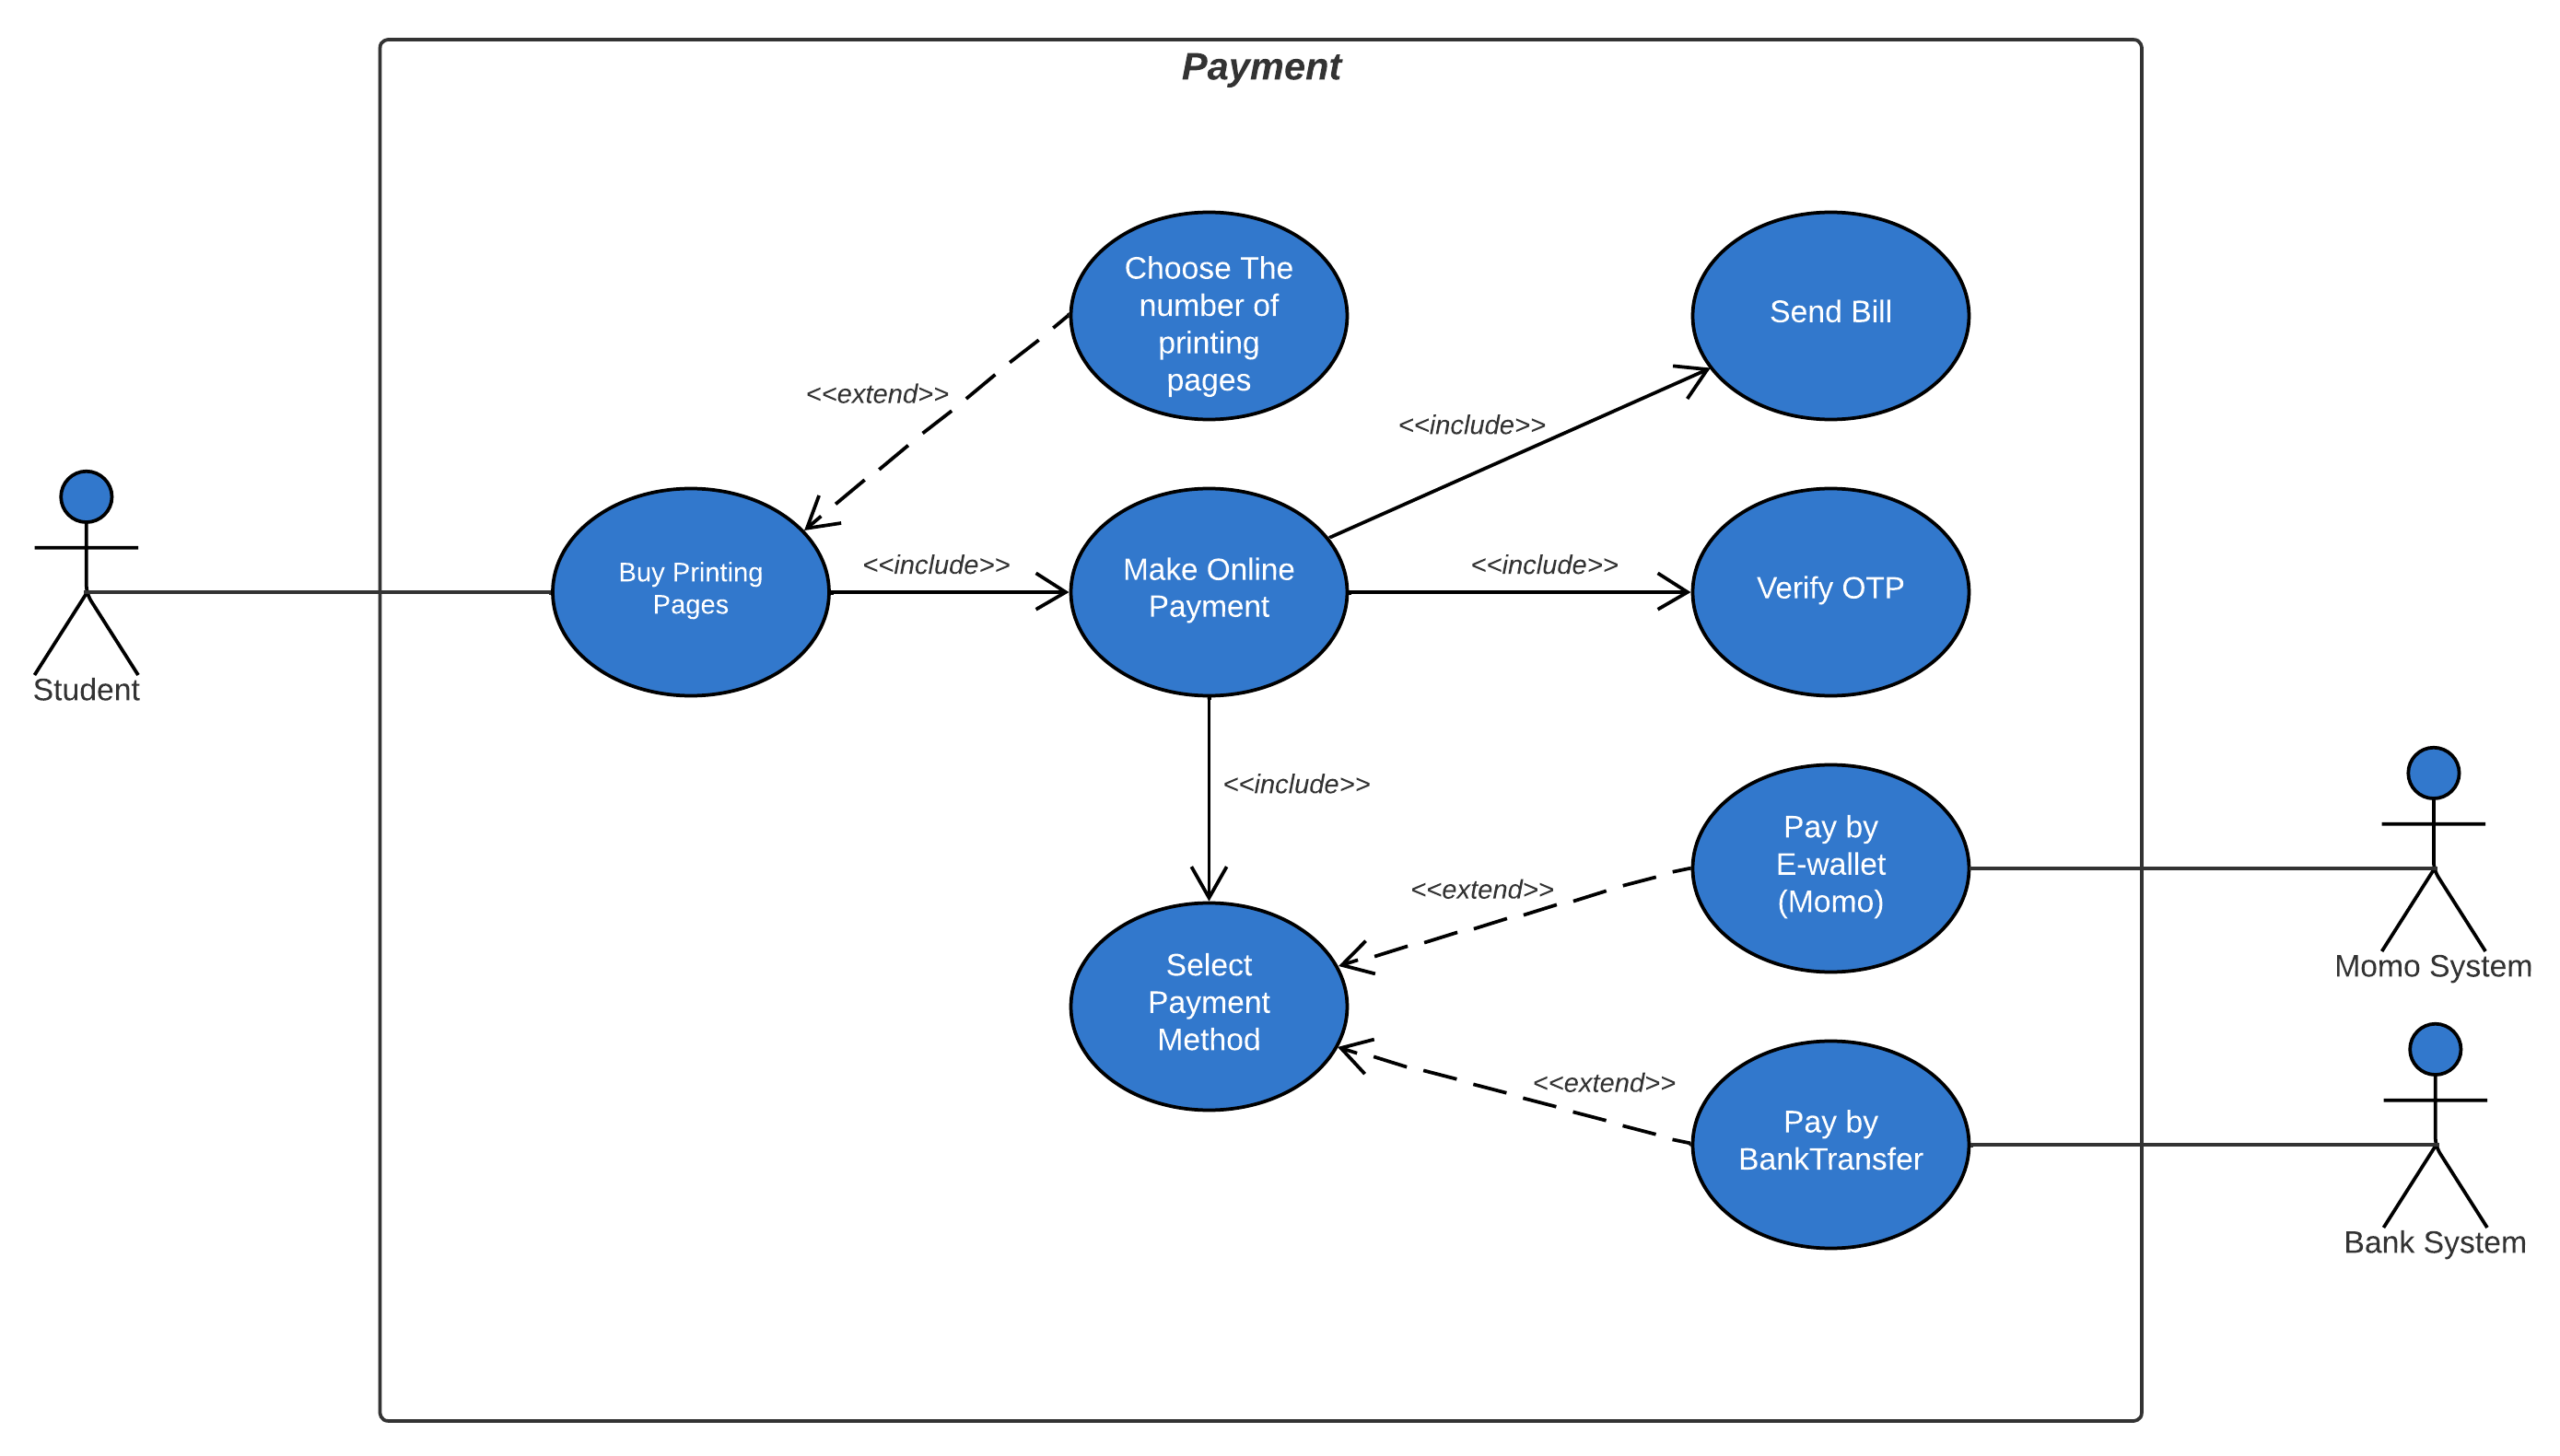
\includegraphics[scale=.62]{images/Task1/payment.png}
    \end{center}
    \label{refhinh1}
    \end{figure}
    \end{center}

    \begin{longtable}{|l|p{10cm}|}
        \hline
        \endhead
        \hline
        \endfoot
        Use-case Name & \textbf{Payment}\\
        \hline
        Actors & Sinh viên, Dịch vụ thanh toán (Hệ thống ngân hàng/ Hệ thống ví điện tử Momo).\\
        \hline
        Description & Use case này mô tả quá trình thanh toán cho giấy in được chọn bởi người dùng. Quá trình này bao gồm lựa chọn số lượng giấy in, cung cấp thông tin thanh toán, xác thực và xử lý thanh toán, sau đó người dùng nhận được xác nhận hoặc biên lai thanh toán.\\
        \hline
        Trigger & Sinh viên nhấn vào nút "Mua giấy in"\\
        \hline
        Pre-conditions & Sinh viên đã đăng nhập vào hệ thống thành công.\\
        \hline
        Post-conditions & - Cập nhật số lượng giấy in của sinh viên.\\
        & - Tài khoản sinh viên bị trừ số tiền tương ứng với số đã thanh toán.\\
        & - Đơn hàng được ghi nhận và lưu trữ.\\
        \hline
        Basic Flow & 1. Sinh viên nhấn vào nút "Mua giấy in".\\
        & 2. Sinh viên chọn số lượng trang giấy cần mua.\\
        & 3. Hệ thống tính toán tổng số tiền cần thanh toán dựa trên số lượng trang và giá in hiện tại.\\
        & 4. Sinh viên chọn phương thức thanh toán từ danh sách các phương thức có sẵn (ví điện tử, chuyển khoản ngân hàng).\\
        & 5. Sinh viên cung cấp chi tiết thanh toán cho phương thức đã chọn.\\
        & 6. Hệ thống gửi yêu cầu thanh toán đến Dịch vụ thanh toán.\\
        & 7. Dịch vụ thanh toán xử lý thanh toán và trả kết quả về cho hệ thống.\\
        & 8. Hệ thống cập nhật số lượng giấy in còn lại của sinh viên và trừ số tiền tương ứng từ tài khoản của họ.\\
        & 9. Đơn hàng được ghi nhận và lưu trữ trong hệ thống.\\
        & 10. Hệ thống hiển thị xác nhận mua thành công và biên lai thanh toán cho sinh viên.\\
        \hline
        Alternative Flow & Alternative 1: Sau bước 6, nếu thanh toán bị sai thông tin:\\
        & \hspace{1em} 6a.1. Hệ thống báo lỗi về thanh toán \\
        & \hspace{1em} 6a.2. Sinh viên ấn vào nút "Thanh toán lại".\\
        &\hspace{1em} Use case quay trở lại bước 6.
        \\
        \hline
        Exception Flow & Exception 1: Nếu sau bước 6, số tiền trong tài khoản sinh viên không đủ:\\
        & \hspace{1em} 6b.1. Hiển thị thông báo thanh toán thất bại.\\
        &\hspace{1em} Use case dừng lại.\\
        &\\
        & Exception 2: Nếu sau bước 10, nếu sinh viên không nhận được xác nhận hoặc biên lai thanh toán: \\
        & \hspace{1em} 10.1. Hệ thống cung cấp cách truy cập lại thông tin thanh toán để sinh viên kiểm tra lại.\\
        &\hspace{1em} Use case dừng lại.\\
        &\\
        & Exception 3: Nếu sau bước 6a.2, nếu sinh viên ấn vào nút "Hủy" thì hủy dịch vụ mua và trở về trang chủ.\\
        &\hspace{1em} Use case dừng lại.\\
    \end{longtable}
    
    \newpage
    \item{\textbf{Manage Printers}}
    \begin{center}
    \begin{figure}[htp]
    \begin{center}
     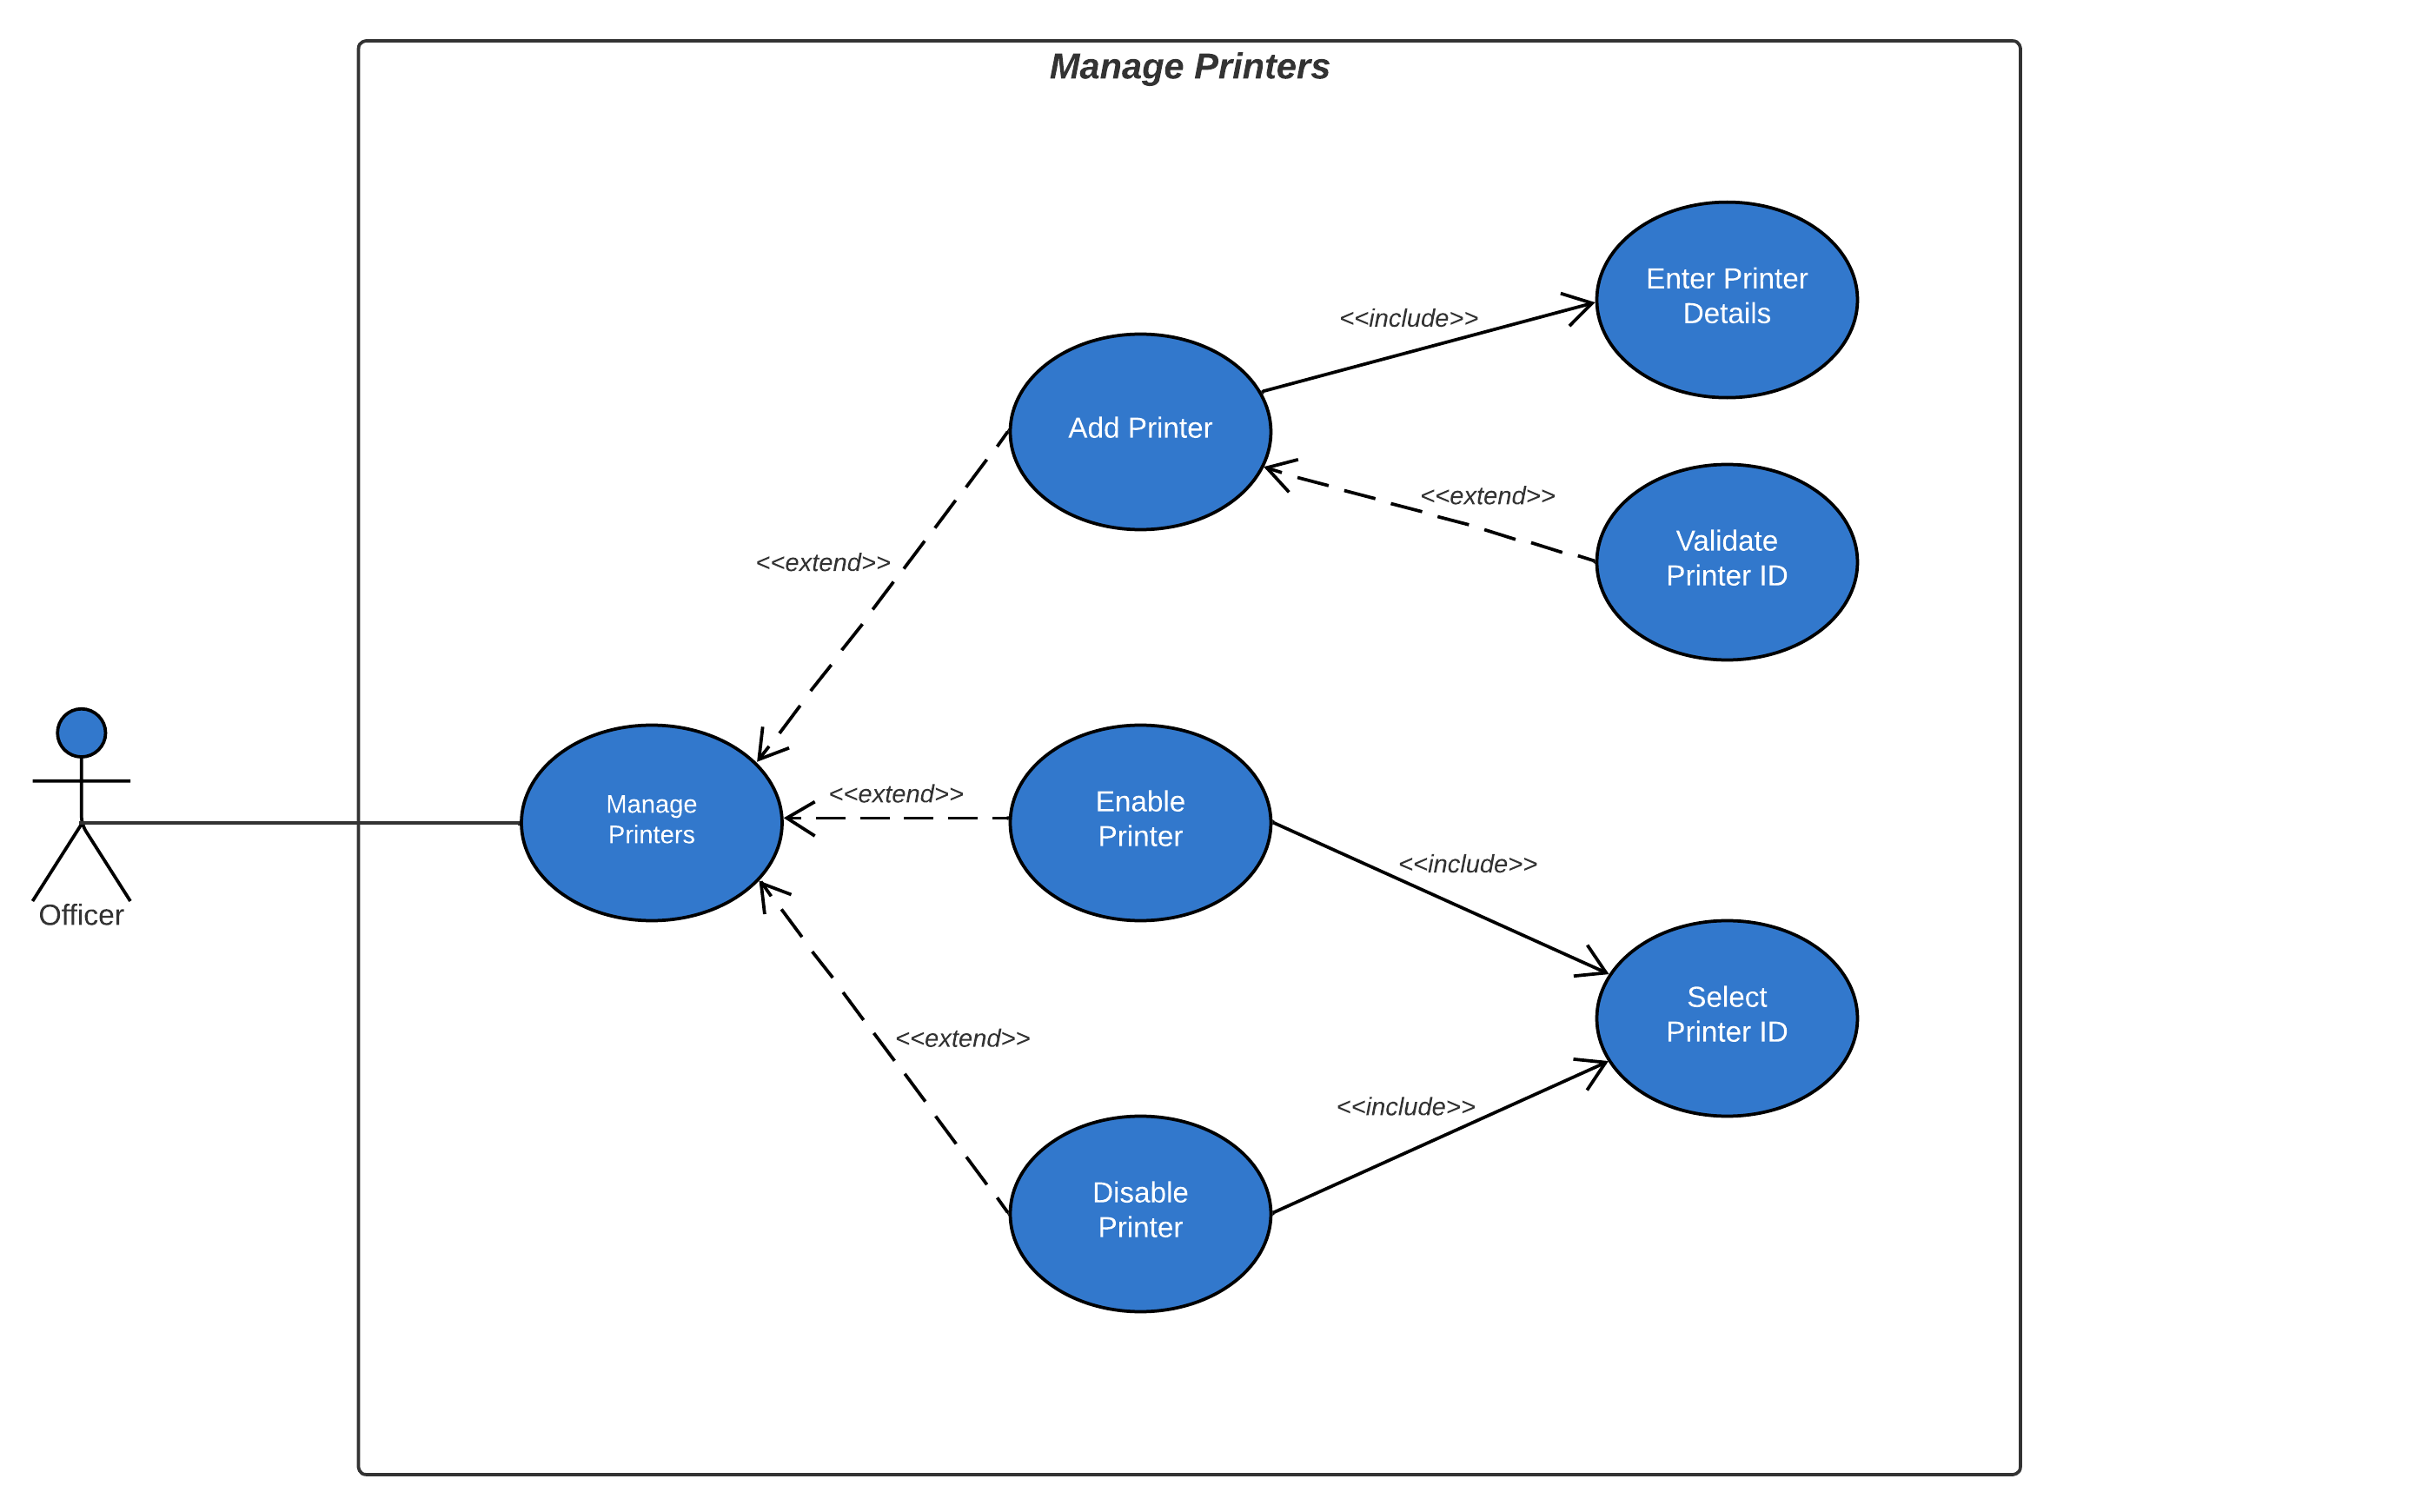
\includegraphics[scale=.62]{images/Task1/managePrinters.png}
    \end{center}
    \label{refhinh1}
    \end{figure}
    \end{center}

    \begin{longtable}{|l|p{10cm}|}
        \hline
        \endhead
        \hline
        \endfoot
        Use-case Name & \textbf{Manage Printers}\\
        \hline
        Actors & Student Printing Service Officer (SPSO) \\
        \hline
        Description & SPSO có thể quản lý các máy in qua những hành động như thêm máy in, bật máy in, tắt máy in và thay đổi cấu hình máy in.
        \\
        \hline
        Trigger 
            & - Lắp đặt thêm máy in: Khi trường đại học lắp đặt thêm máy in, SPSO có trách nhiệm thêm máy in đó vào hệ thống SPSS. \\
            & - Bảo trì máy in: Khi máy in có sự cố, SPSO tắt máy in, tạm thời loại máy in ra khỏi hệ thống đang hoạt động để kiểm tra, sửa chữa. Khi đã hoàn tất, SPSO có thể bật máy in và thêm vào hệ thống máy in đang hoạt động.
        \\
        \hline
        Pre-conditions &  
            - Người dùng (SPSO) phải được xác thực thông qua hệ thống đăng nhập HCMUT\_SSO. \\ &
            - SPSO phải có quyền truy cập vào hệ thống quản lý máy in. \\ &
            - Mỗi máy in chỉ được phép có một ID duy nhất (không trùng lặp). \\ &
            - Máy in phải có ID đang hoạt động trong hệ thống để bật hoặc tắt. \\ &
            - Hệ thống máy in đang hoạt động.
        \\
        \hline
        Post-conditions & None.\\
        \hline
        Basic Flow & 
            1. SPSO đăng nhập vào hệ thống quản lý máy in qua HCMUT\_SSO. \\ &
            2. SPSO chọn một trong ba chức năng: Thêm máy in, bật máy in, tắt máy in.
        \\
        \hline
        Alternative Flow & Alternative 1: Sau bước 2, nếu SPSO chọn chức năng thêm máy in:\\
        & \hspace{1em} 2a.1. SPSO xác nhận máy in vật lý đã được lắp đặt và kết nối điện.\\
        & \hspace{1em} 2a.2. SPSO sẽ gán một ID cố định cho máy in\\
        & \hspace{1em} 2a.3. SPSO sẽ đưa các hiệu chỉnh mặc định của hệ thống vào trong máy in.\\
        & \hspace{1em} 2a.4. SPSO sẽ điền các thông tin của máy in vào hệ thống (tên máy in, địa điểm, ...).\\
        &\\
        &Alternative 2: Sau bước 2, nếu SPSO chọn chức năng tắt máy in:\\
        & \hspace{1em} 2b.1. SPSO xác nhận máy in thông qua ID của máy in đó.\\
        & \hspace{1em} 2b.2. SPSO loại máy in đó khỏi hệ thống SPSS.\\
        &\\
        &Alternative 3: Sau bước 2, nếu SPSO chọn chức năng tắt máy in:\\
        & \hspace{1em} 2c.1. SPSO xác nhận máy in thông qua ID của máy in đó.\\
        & \hspace{1em} 2c.2. SPSO thêm lại máy in đó vào hệ thống SPSS.\\
        \hline
        Exception Flow & Exception 1: SPSO có thể chọn lại ID nếu ID ban đầu không đúng với máy in cần thêm / bớt hoặc ID không tồn tại\\
        &\\
         & Exception 2: SPSO có thể gán lại ID cho máy in mới nếu ID được chọn đã tồn tại sẵn trong hệ thống.\\
    \end{longtable}
    
    \newpage
    \item{\textbf{Configure System}}
    \begin{center}
    \begin{figure}[htp]
    \begin{center}
     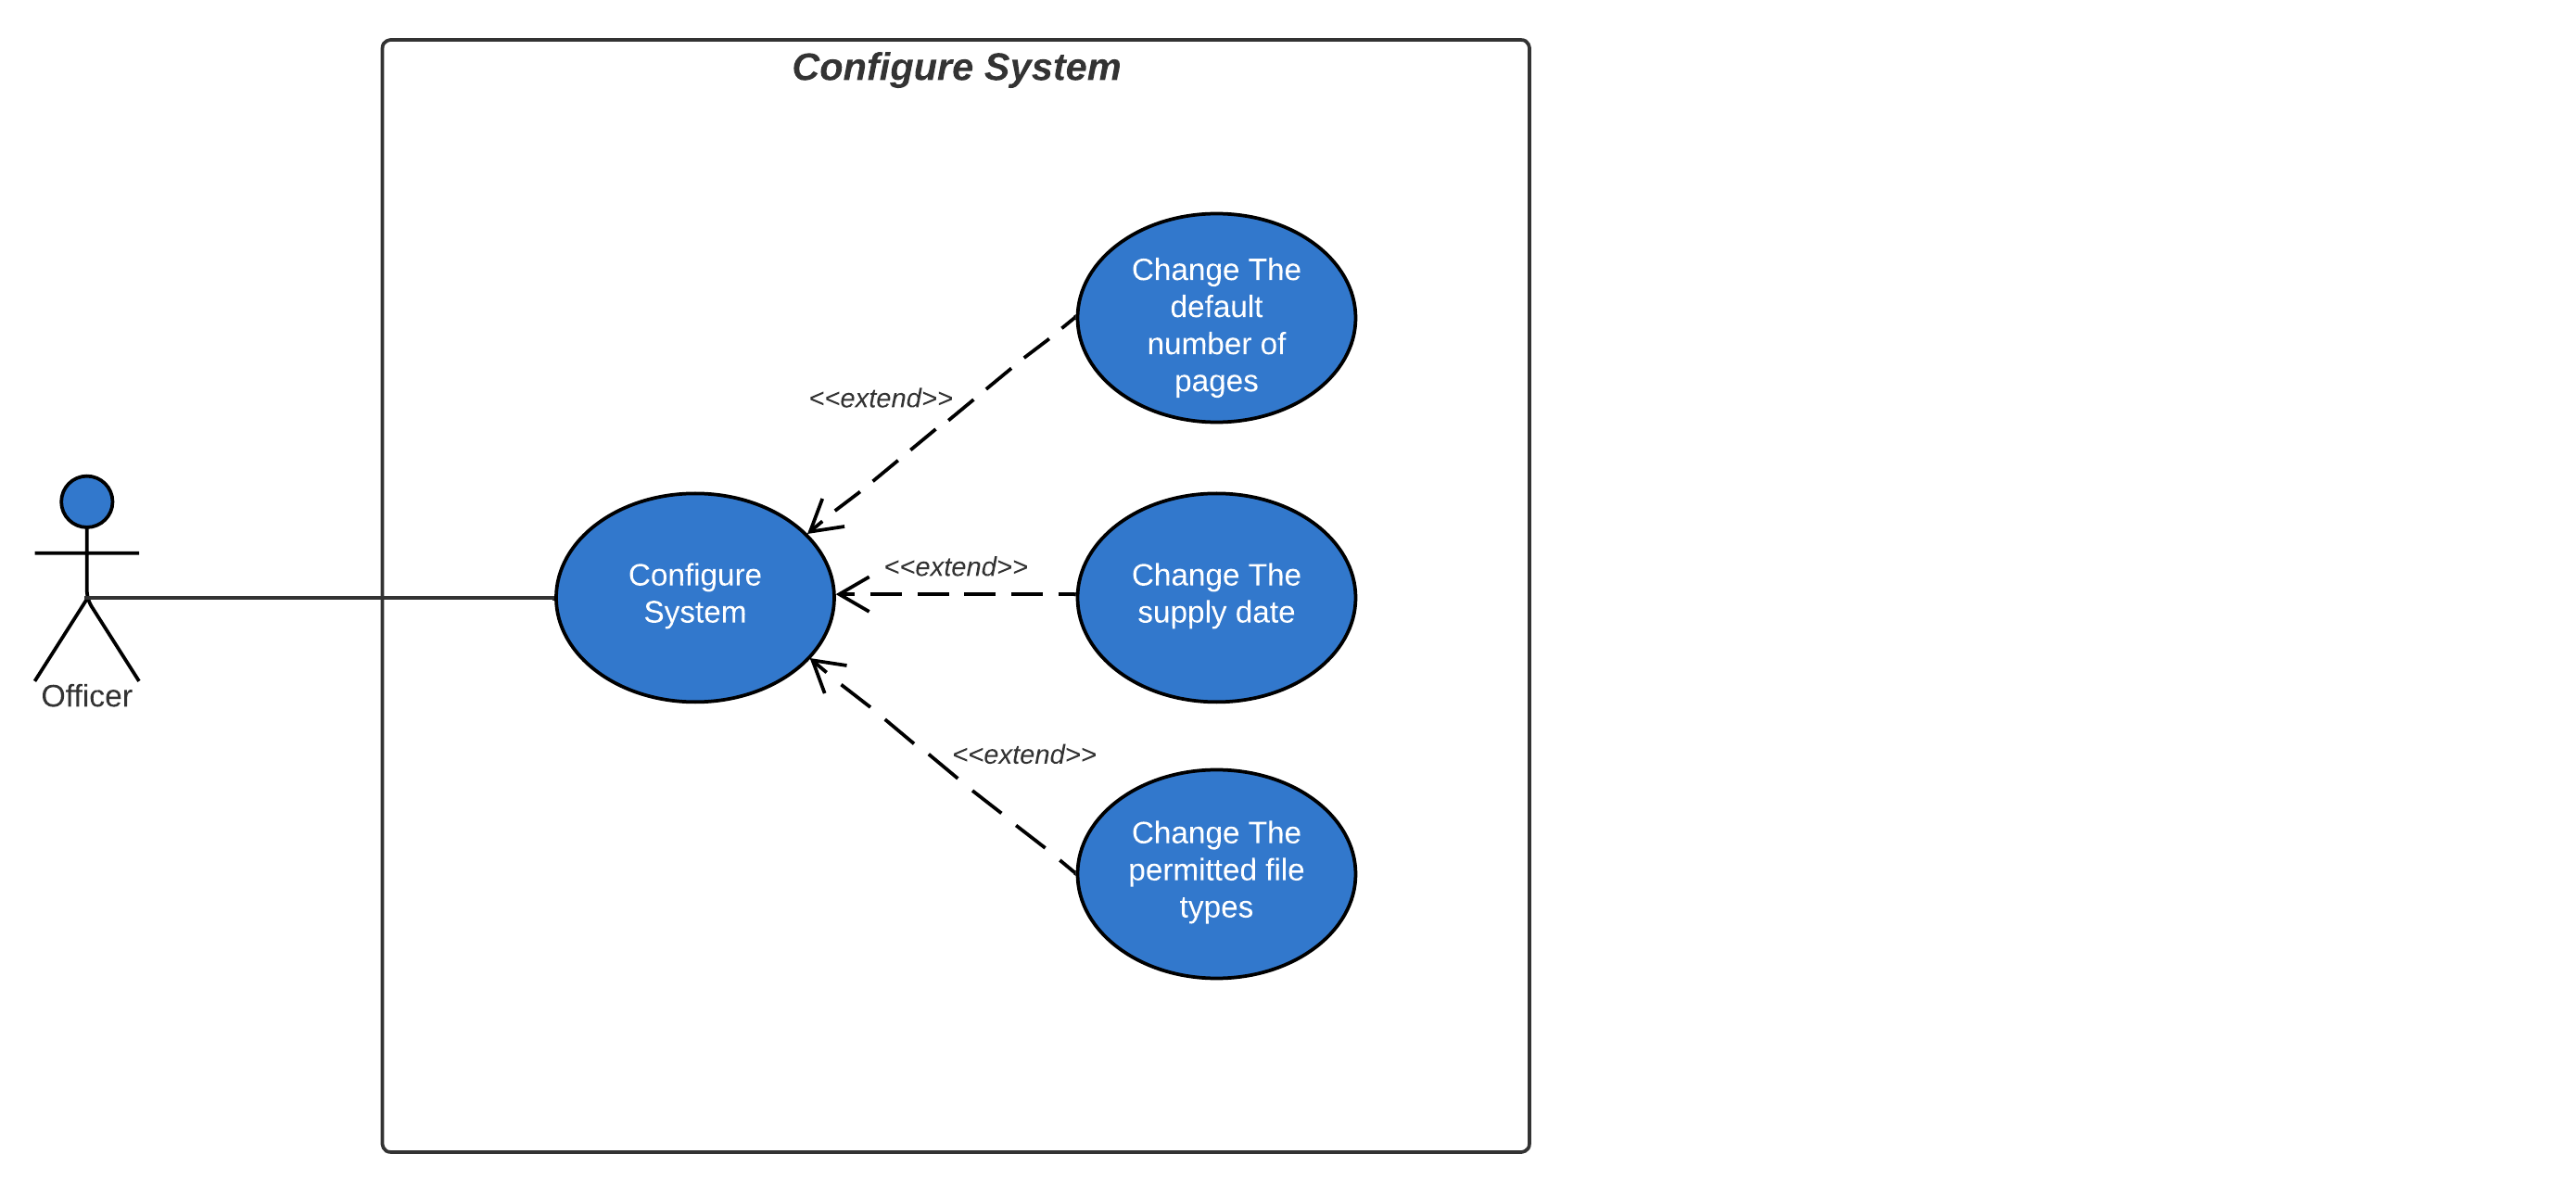
\includegraphics[scale=.62]{images/Task1/configureSystem.png}
    \end{center}
    \label{refhinh1}
    \end{figure}
    \end{center}

    \begin{longtable}{|l|p{10cm}|}
        \hline
        \endhead
        \hline
        \endfoot
        Use-case Name & \textbf{Configure System}\\
        \hline
        Actors & Student Printing Service Officer (SPSO)\\
        \hline
        Description & SPSO có quyền thay đổi các tùy chỉnh của hệ thống bao gồm số lượng tờ giấy mặc định, thời điểm mà hệ thống cung cấp cho tất cả sinh viên một số lượng giấy in mặc định, các định dạng tập tin được chấp nhận bởi hệ thống.\\
        \hline
        Trigger & Khi SPSO chọn chức năng Configure system trong trang chính của phần mềm quản lý hệ thống máy in.\\
        \hline
        Pre-conditions & SPSO phải đăng nhập thành công vào hệ thống\\
        \hline
        Post-conditions & - Giao diện để thay đổi các tùy chỉnh của hệ thống sẽ hiện lên.\\
        & - SPSO cập nhật thành công số lượng giấy in mặc định, thời điểm mà hệ thống cung cấp cho tất cả sinh viên một số lượng giấy in mặc định, các định dạng tập tin được chấp nhận bởi hệ thống.\\
        \hline
        Basic Flow & 1. SPSO đăng nhập vào hệ thống quản lý máy in HCMUT\_SSO\\
        & 2. SPSO chọn chức năng Configure system trong trang chính của phần mềm quản lý hệ thống máy in.\\
        & 3. SPSO chọn một trong ba chức năng: tùy chỉnh số lượng giấy in mặc định, tùy chỉnh thời điểm hệ thống cung cấp cho tất cả sinh viên một số lượng giấy in mặc định hoặc tùy chỉnh các định dạng tập tin được chấp nhận bởi hệ thống.\\
        & 4. Trong trang chức năng, SPSO nhấn nút lưu để cập nhật thông tin được thay đổi, một bảng thông báo "Cập nhật thành công" sẽ hiện lên, SPSO nhấn nút OK để tắt.\\
        \hline
        Alternative Flow & Alternative 1: Sau bước 3, Nếu SPSO chọn chức năng tùy chỉnh số lượng giấy in mặc định.\\
        & \hspace{1em} 3a.1. SPSO có thể nhập số lượng giấy in mặc định mới. \\
        & \hspace{1em} 3a.2. SPSO nhấn nút lưu để cập nhật thay đổi.\\
        
        &Alternative 2: Sau bước 3, Nếu SPSO chọn chức năng tùy chỉnh thời điểm hệ thống cung cấp cho tất cả sinh viên một số lượng giấy in mặc định:\\
        & \hspace{1em} 3b.1. SPSO có thể thay đổi các thông số của thời điểm nêu trên bao gồm giờ, phút, giây, ngày, tháng và năm thông qua các drop down list.\\
        & \hspace{1em} 3b.2. SPSO bấm nút lưu để cập nhật thay đổi.\\
        &\\
        &Alternative 3: Sau bước 3, Nếu SPSO chọn chức năng tùy chỉnh các định dạng tập tin được chấp nhận bởi hệ thống:\\
        & \hspace{1em} 3c.1. SPSO thêm hoặc xóa bớt một định dạng tập tin trong danh sách các tập tin được hệ thống chấp nhận.\\
        & \hspace{1em} 3c.2. SPSO bấm nút lưu để cập nhật thay đổi.\\
        \hline
        Exception Flow & Exception 1: Sau bước 2, SPSO có thể nhấn nút quay lại để trở về trang chính của phần mềm quản lý hệ thống máy in.\\
        &\\
        & Exception 2: Sau bước 3, SPSO có thể nhấn nút hủy để quay lại màn hình chọn chức năng cần tùy chỉnh.\\
        &\\
        & Exception 3: Ở luồng sự kiện phụ 3a.1, nếu SPSO nhập số lượng giấy in không hợp lệ và nhấn lưu, một bảng thông báo "số lượng giấy in không hợp lệ" sẽ hiện lên, SPSO nhấn nút OK để quay lại luồng sự kiện phụ 3a.1.\\
        &\\
        & Exception 4: ở luồng sự kiện phụ 3c.1, nếu SPSO thêm một định dạng tập tin không hợp lệ và nhấn lưu, một bảng thông báo "định dạng không hợp lệ" sẽ hiện lên, SPSO nhấn nút OK để quay lại luồng sự kiện phụ 3c.1\\
    \end{longtable}

    
    \newpage
    \item{\textbf{Log In}}
    \begin{center}
    \begin{figure}[!htp]
    \begin{center}
     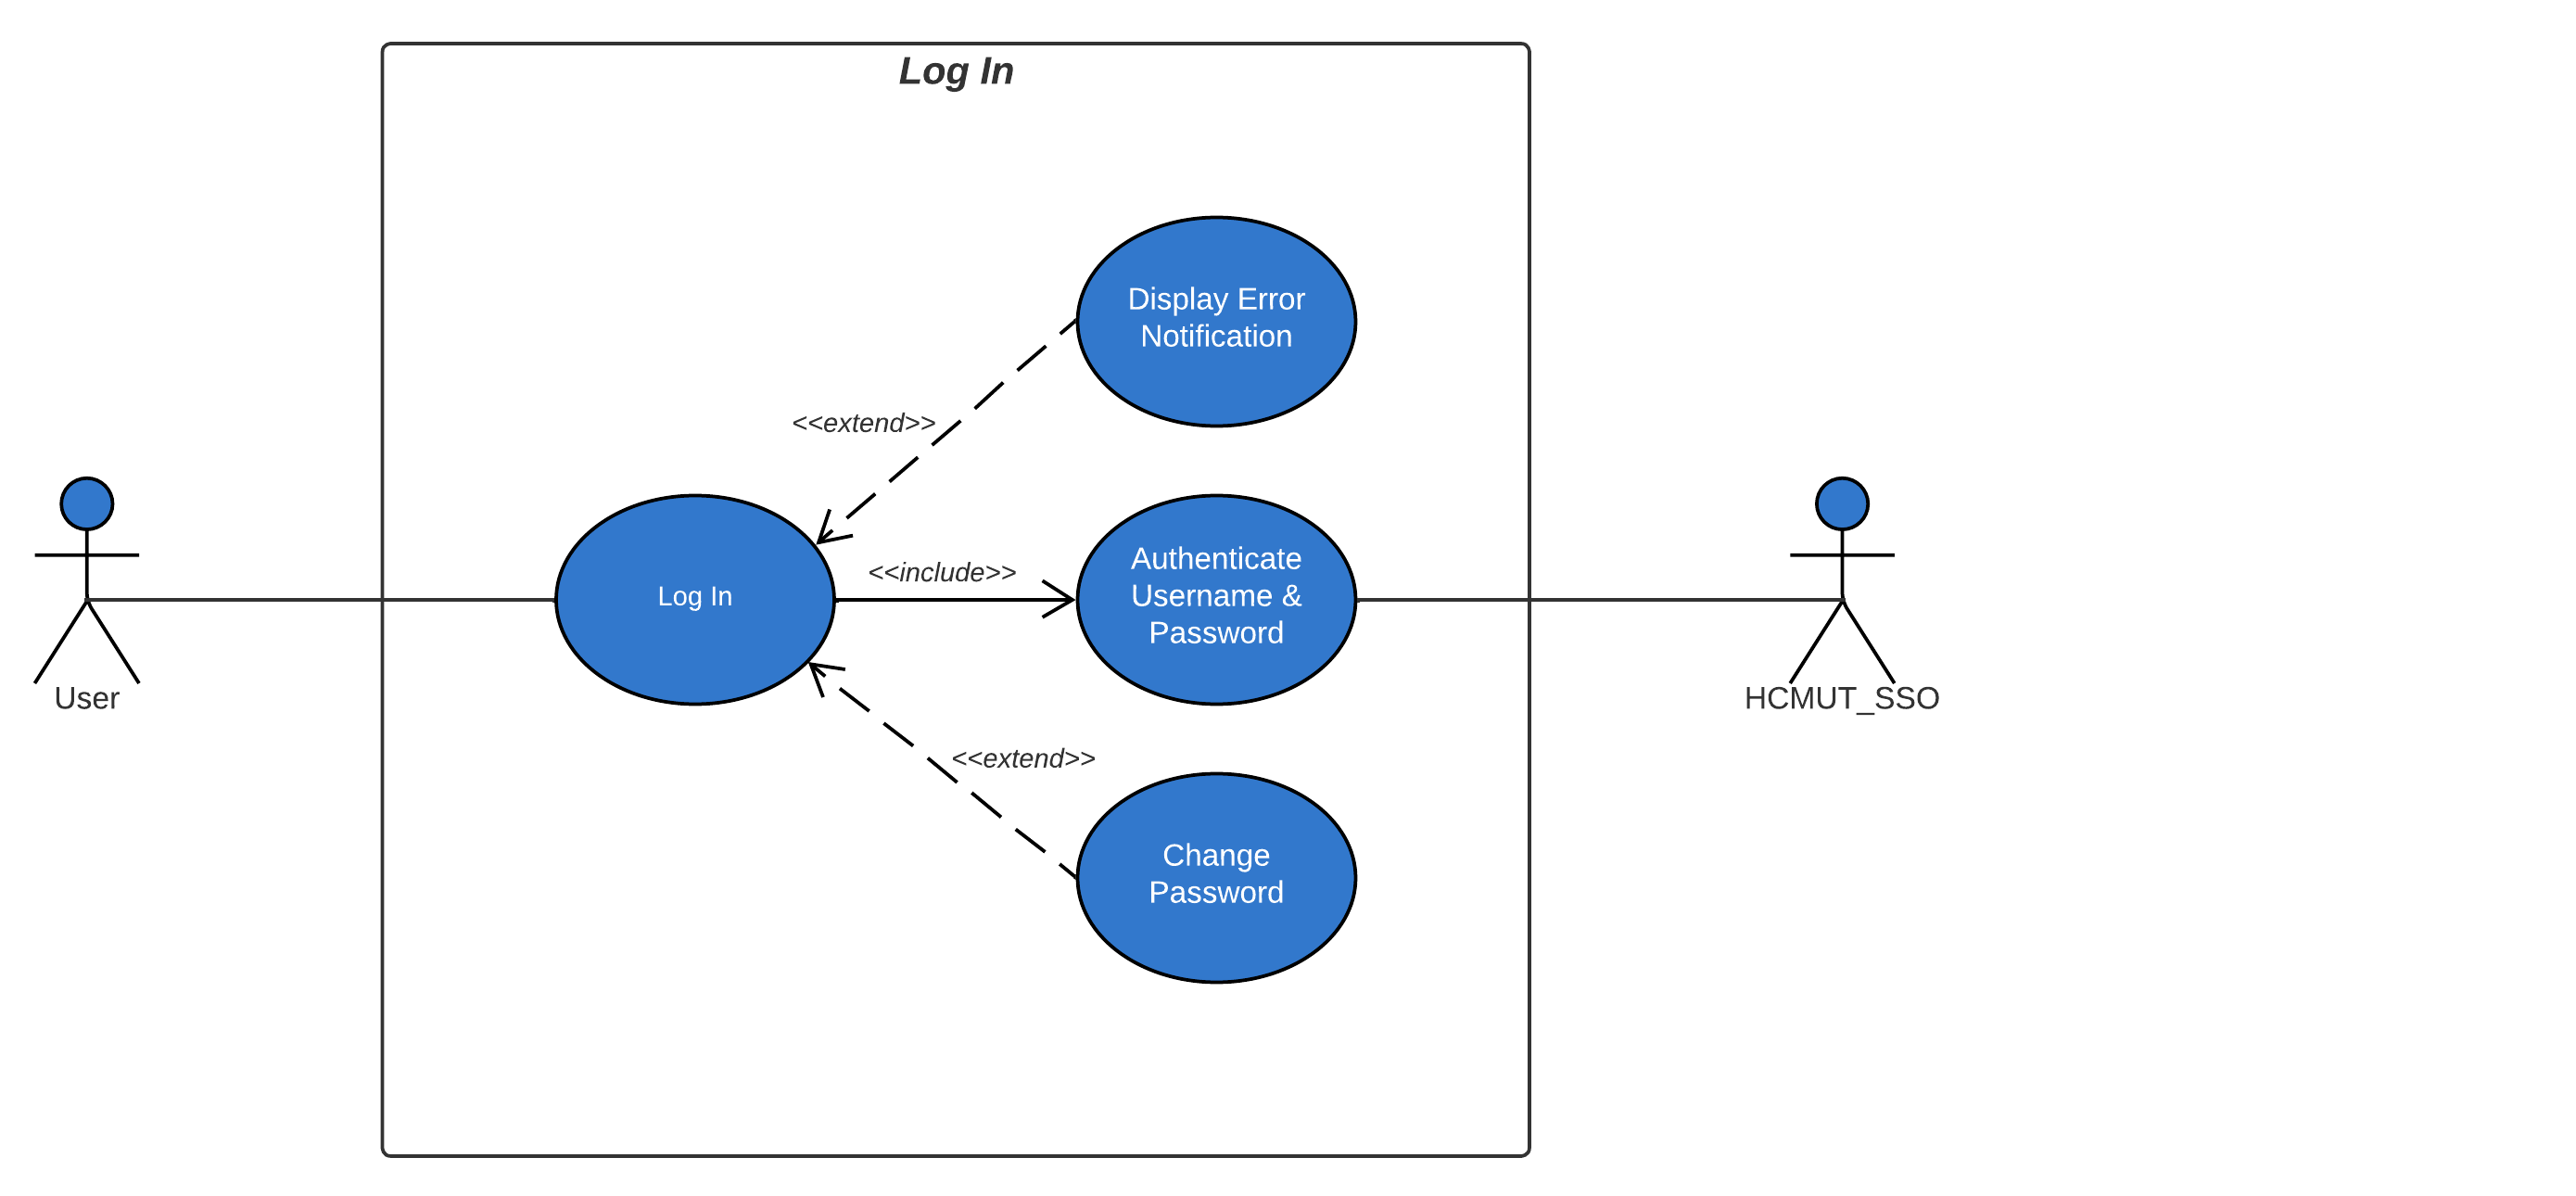
\includegraphics[scale=.62]{images/Task1/login.png}
    \end{center}
    \label{refhinh1}
    \end{figure}
    \end{center}

    \begin{longtable}{|l|p{10cm}|}
        \hline
        \endhead
        \hline
        \endfoot
        Use-case Name & \textbf{Log In}\\
        \hline
        Actors & Sinh viên, Student Printing Service Officer. \\
        \hline
        Description & Người dùng thực hiện việc đăng nhập vào hệ thống.\\
        \hline
        Trigger & Người dùng truy cập trang đăng nhập và bắt đầu nhập thông tin đăng nhập.\\
        \hline
        Pre-conditions & - Tài khoản của người dùng đã được tạo.\\
                       & - Tài khoản của người dùng đã được phân quyền.\\
                       & - Thiết bị của người dùng đã được kết nối internet khi thực hiện đăng nhập.\\
        \hline
        Post-conditions & Người dùng đăng nhập thành công và có thể sử dụng những chức năng của hệ thống\\
        \hline
        Basic Flow & 1. Người dùng truy cập trang đăng nhập.\\
        & 2. Người dùng nhập tài khoản và mật khẩu.\\
        & 3. Hệ thống xác thực thông tin đăng nhập thành công và cho phép người dùng truy cập ứng dụng.\\
        & 4. Hệ thống ghi nhận hoạt động đăng nhập thành công \\
        \hline
        Alternative Flow & None.\\
        \hline
        Exception Flow & Exception 1: Ở bước 3, nếu tài khoản hoặc mật khẩu sai:\\
        & \hspace{1em} 3.1. Hệ thống hiển thị thông báo sai tài khoản hoặc mật khẩu.\\
        & \hspace{1em} 3.2. Hệ thống quay về trang đăng nhập. \\
        &\hspace{1em} Use case dừng lại.\\
        
        & Exception 2: Sau bước 1, nếu người dùng chọn đổi mật khẩu:\\
        & \hspace{1em} 1.1. Hiển thị trang đổi mật khẩu bao gồm 4 trường nhập tài khoản, nhập mật khẩu cũ, nhập mật khẩu mới và xác nhận mật khẩu mới. \\
        & \hspace{1em} 1.2. Nếu thông tin đúng thì mật khẩu được thay đổi.\\
        &\hspace{1em} Use case dừng lại.\\
    \end{longtable}
    \end{enumerate}
        
	%%%%%%%%%%%%%%%%%%%%%%%%%%%%%%%%%
        \newpage
	\section{Task 2: System modelling}
        \subsection{Task 2.1: Activity diagrams}

    \subsubsection{Request For Printing Service}
    \begin{center}
    \begin{figure}[!htp]
    \begin{center}
     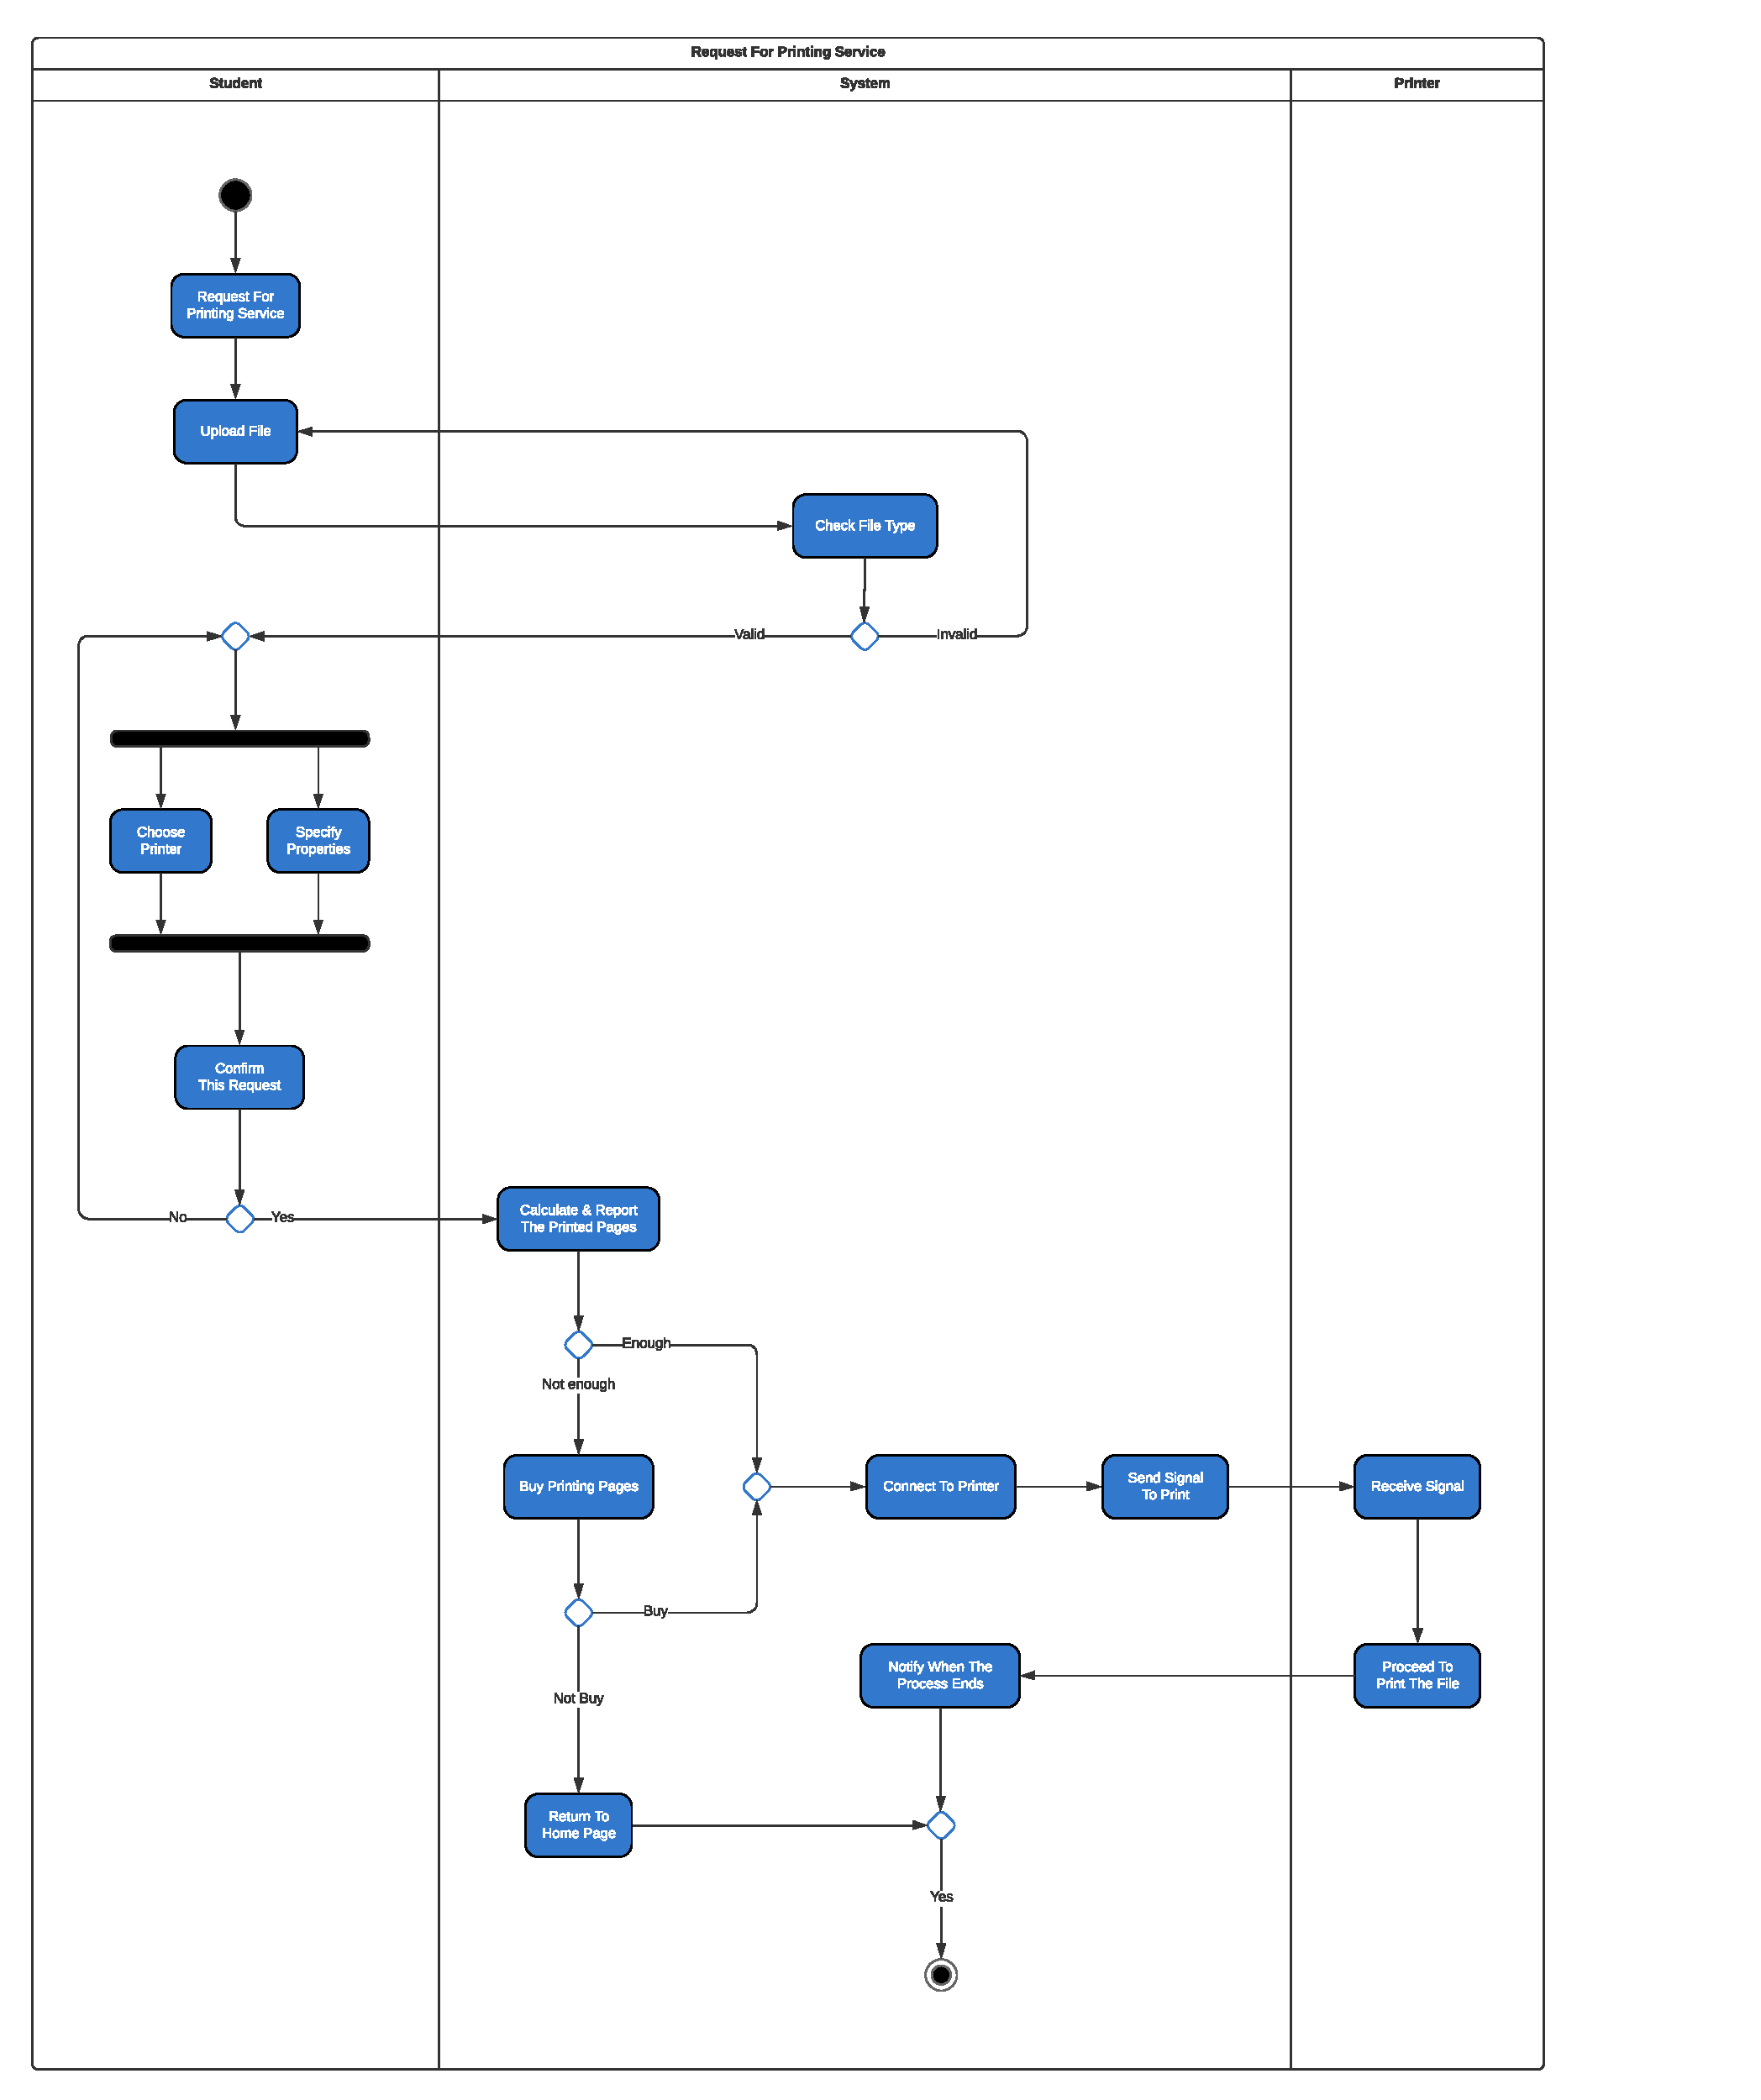
\includegraphics[scale=.4]{images/Task2/ActivityDiagrams/RequestForPrintingService.pdf}
    \end{center}
    \label{refhinh1}
    \end{figure}
    \end{center}
    \newpage
    \textbf{Mô tả:}
    \begin{itemize}
        \item Sinh viên chọn dịch vụ in và tải file cần in lên hệ thống, hệ thống sẽ kiểm tra tính hợp lệ của file:
        \begin{itemize}
            \item Nếu file hợp lệ thì sinh viên sẽ được tiến hành bước tiếp theo.
            \item Nếu file không hợp lệ hệ thống sẽ quay lại bước tải file để sinh viên tải tệp tin khác lên.
        \end{itemize}
        \item Sau khi tải tệp lên sinh viên chọn máy in và cấu hình các thuộc tính in hoặc để mặc định hệ thống.
        \item Sinh viên cần xác nhận để hệ thống tiếp tục bước tiếp theo, bước này nhằm tránh việc sinh viên quên cấu hình các thuộc tính mình cần.
        \item Sau đó hệ thống sẽ tính toán lại số trang mà sinh viên có thể in còn lại và báo cáo lại cho sinh viên:
        \begin{itemize}
            \item Nếu số trang còn lại đủ để phục vụ in tập tin sinh viên vừa tải lên thì hệ thống sẽ tiến hành in cho sinh viên.
            \item Ngược lại, nếu số trang không đủ thì sinh viên được quyền mua thêm hoặc không:
            \begin{itemize}
                \item Nếu sinh viên chọn không mua hệ thống sẽ đưa sinh viên về lại trang chủ.
                \item Nếu sinh viên chọn mua và hoàn tất thanh toán đủ thì hệ thống sẽ tiến hành in tập tin cho sinh viên
            \end{itemize}
        \end{itemize}
        \item Khi đã hoàn thành công việc quản lý máy in, SPSO sẽ đăng xuất hỏi hệ thống.
    \end{itemize}


    \newpage
    \subsubsection{Make Online Payment}
   \begin{center}
    \begin{figure}[!htp]
    \begin{center}
     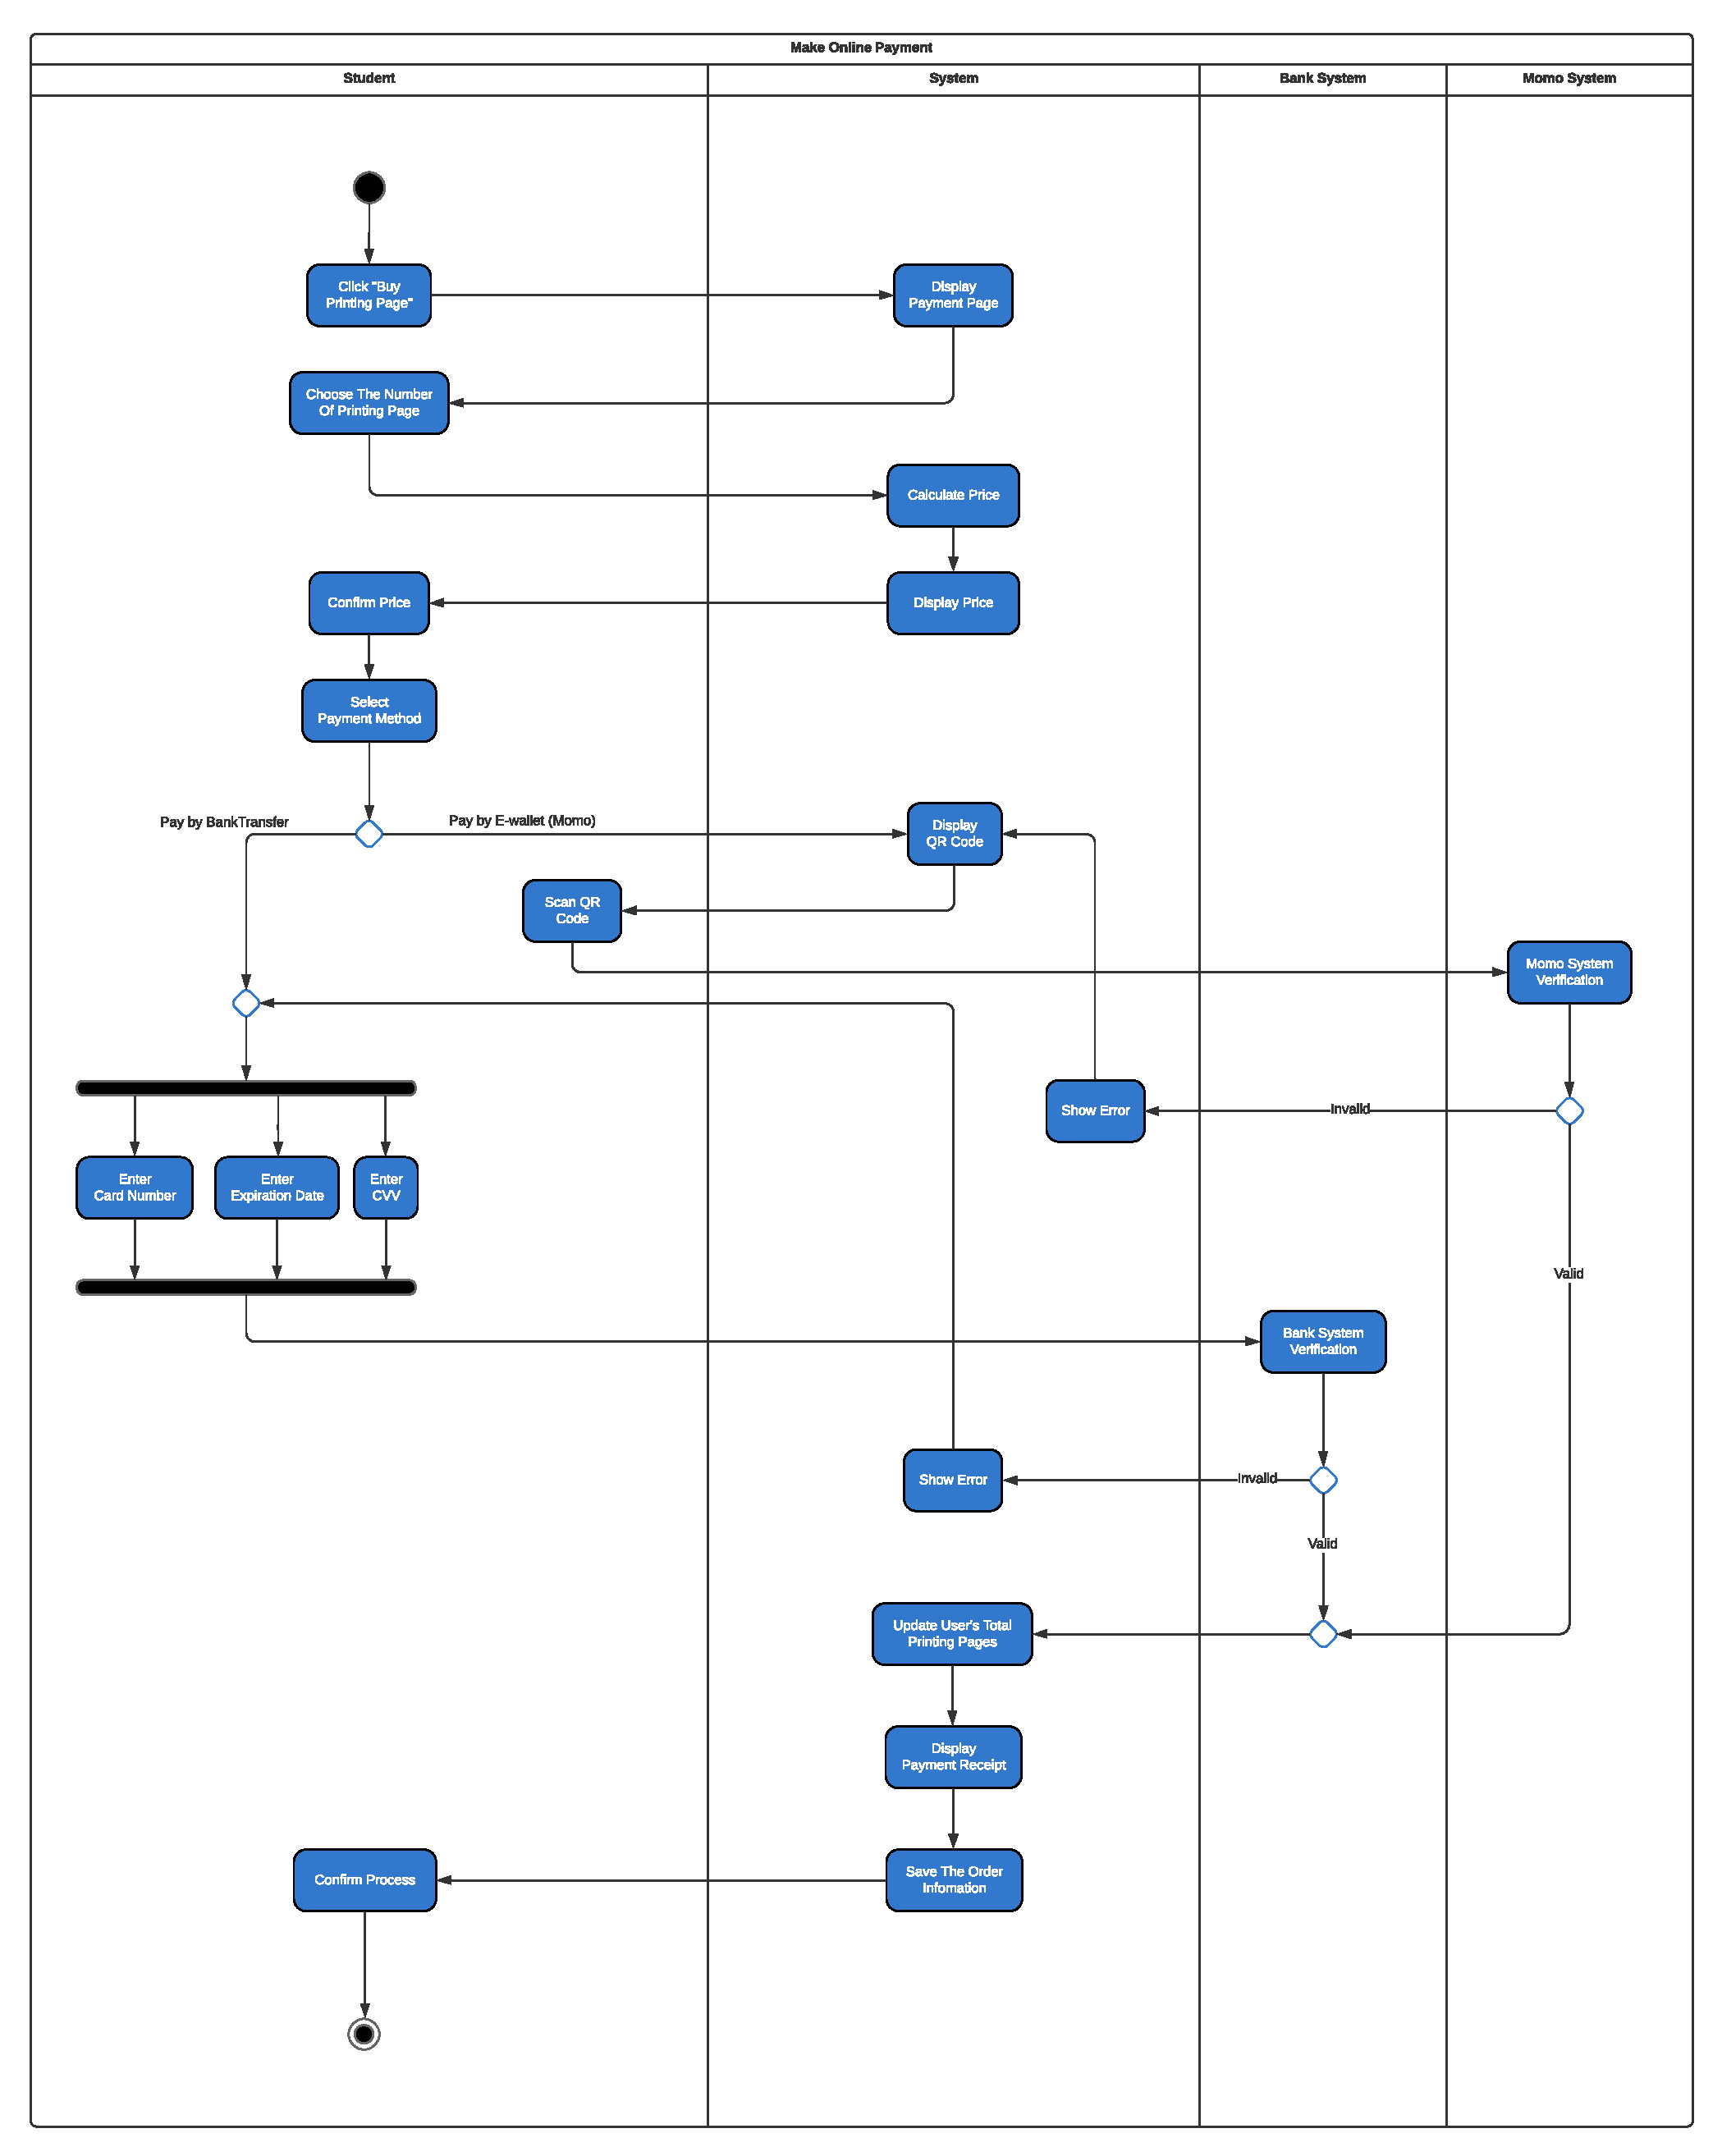
\includegraphics[scale=.4]{images/Task2/ActivityDiagrams/Payment.pdf}
    \end{center}
    \label{refhinh1}
    \end{figure}
    \end{center}
    \newpage
    \textbf{Mô tả:}
    \begin{itemize}
        \item Đầu tiên, khi sinh viên quyết định mua thêm giấy in, họ sẽ lựa chọn dịch vụ mua giấy in trong hệ thống.
        \item Sau khi đăng nhập thành công vào tài khoản của họ, sinh viên có thể tiến hành mua giấy in bằng cách chọn tùy chọn "Mua giấy in." Hệ thống sẽ hiển thị giao diện mua giấy in, nơi sinh viên có thể chỉ định số lượng giấy in mà họ muốn mua.
        \item Hệ thống sẽ dựa vào số lượng giấy in được chọn bởi sinh viên và giá của giấy in tại thời điểm đó để tính toán tổng số tiền cần thanh toán. Sau đó, hiển thị ra màn hình và sinh viên sẽ xem và xác nhận số tiền này.
        \item Sau khi xác nhận giá trị thanh toán, sinh viên có hai lựa chọn thanh toán: sử dụng thẻ Visa hoặc ví điện tử Momo.
        \begin{itemize}
            \item Nếu sinh viên chọn thanh toán bằng thẻ Visa, họ cần cung cấp thông tin thẻ gồm số thẻ, ngày hết hạn và mã bảo vệ. Hệ thống sẽ gửi yêu cầu xác nhận thanh toán đến ngân hàng liên quan.
            \item Nếu sinh viên ưa thích thanh toán qua Momo, hệ thống sẽ hiển thị mã QR. Sinh viên chỉ cần quét mã này, và hệ thống sẽ gửi yêu cầu xác nhận thanh toán đến ví điện tử Momo.
        \end{itemize}
        \item Trong cả hai trường hợp, nếu thanh toán thành công, hệ thống sẽ cập nhật số lượng giấy in trong tài khoản của sinh viên, lưu hóa đơn thanh toán và hiển thị nó để sinh viên có thể xác nhận.
        \item Trong trường hợp thanh toán không thành công, hệ thống sẽ hiển thị thông báo lỗi và đưa quay lại bước thanh toán trước đó để sinh viên có cơ hội sửa lỗi hoặc lựa chọn phương thức thanh toán khác.
    \end{itemize}


    \newpage
    \subsubsection{Manage Printers}
    \begin{center}
    \begin{figure}[!htp]
    \begin{center}
     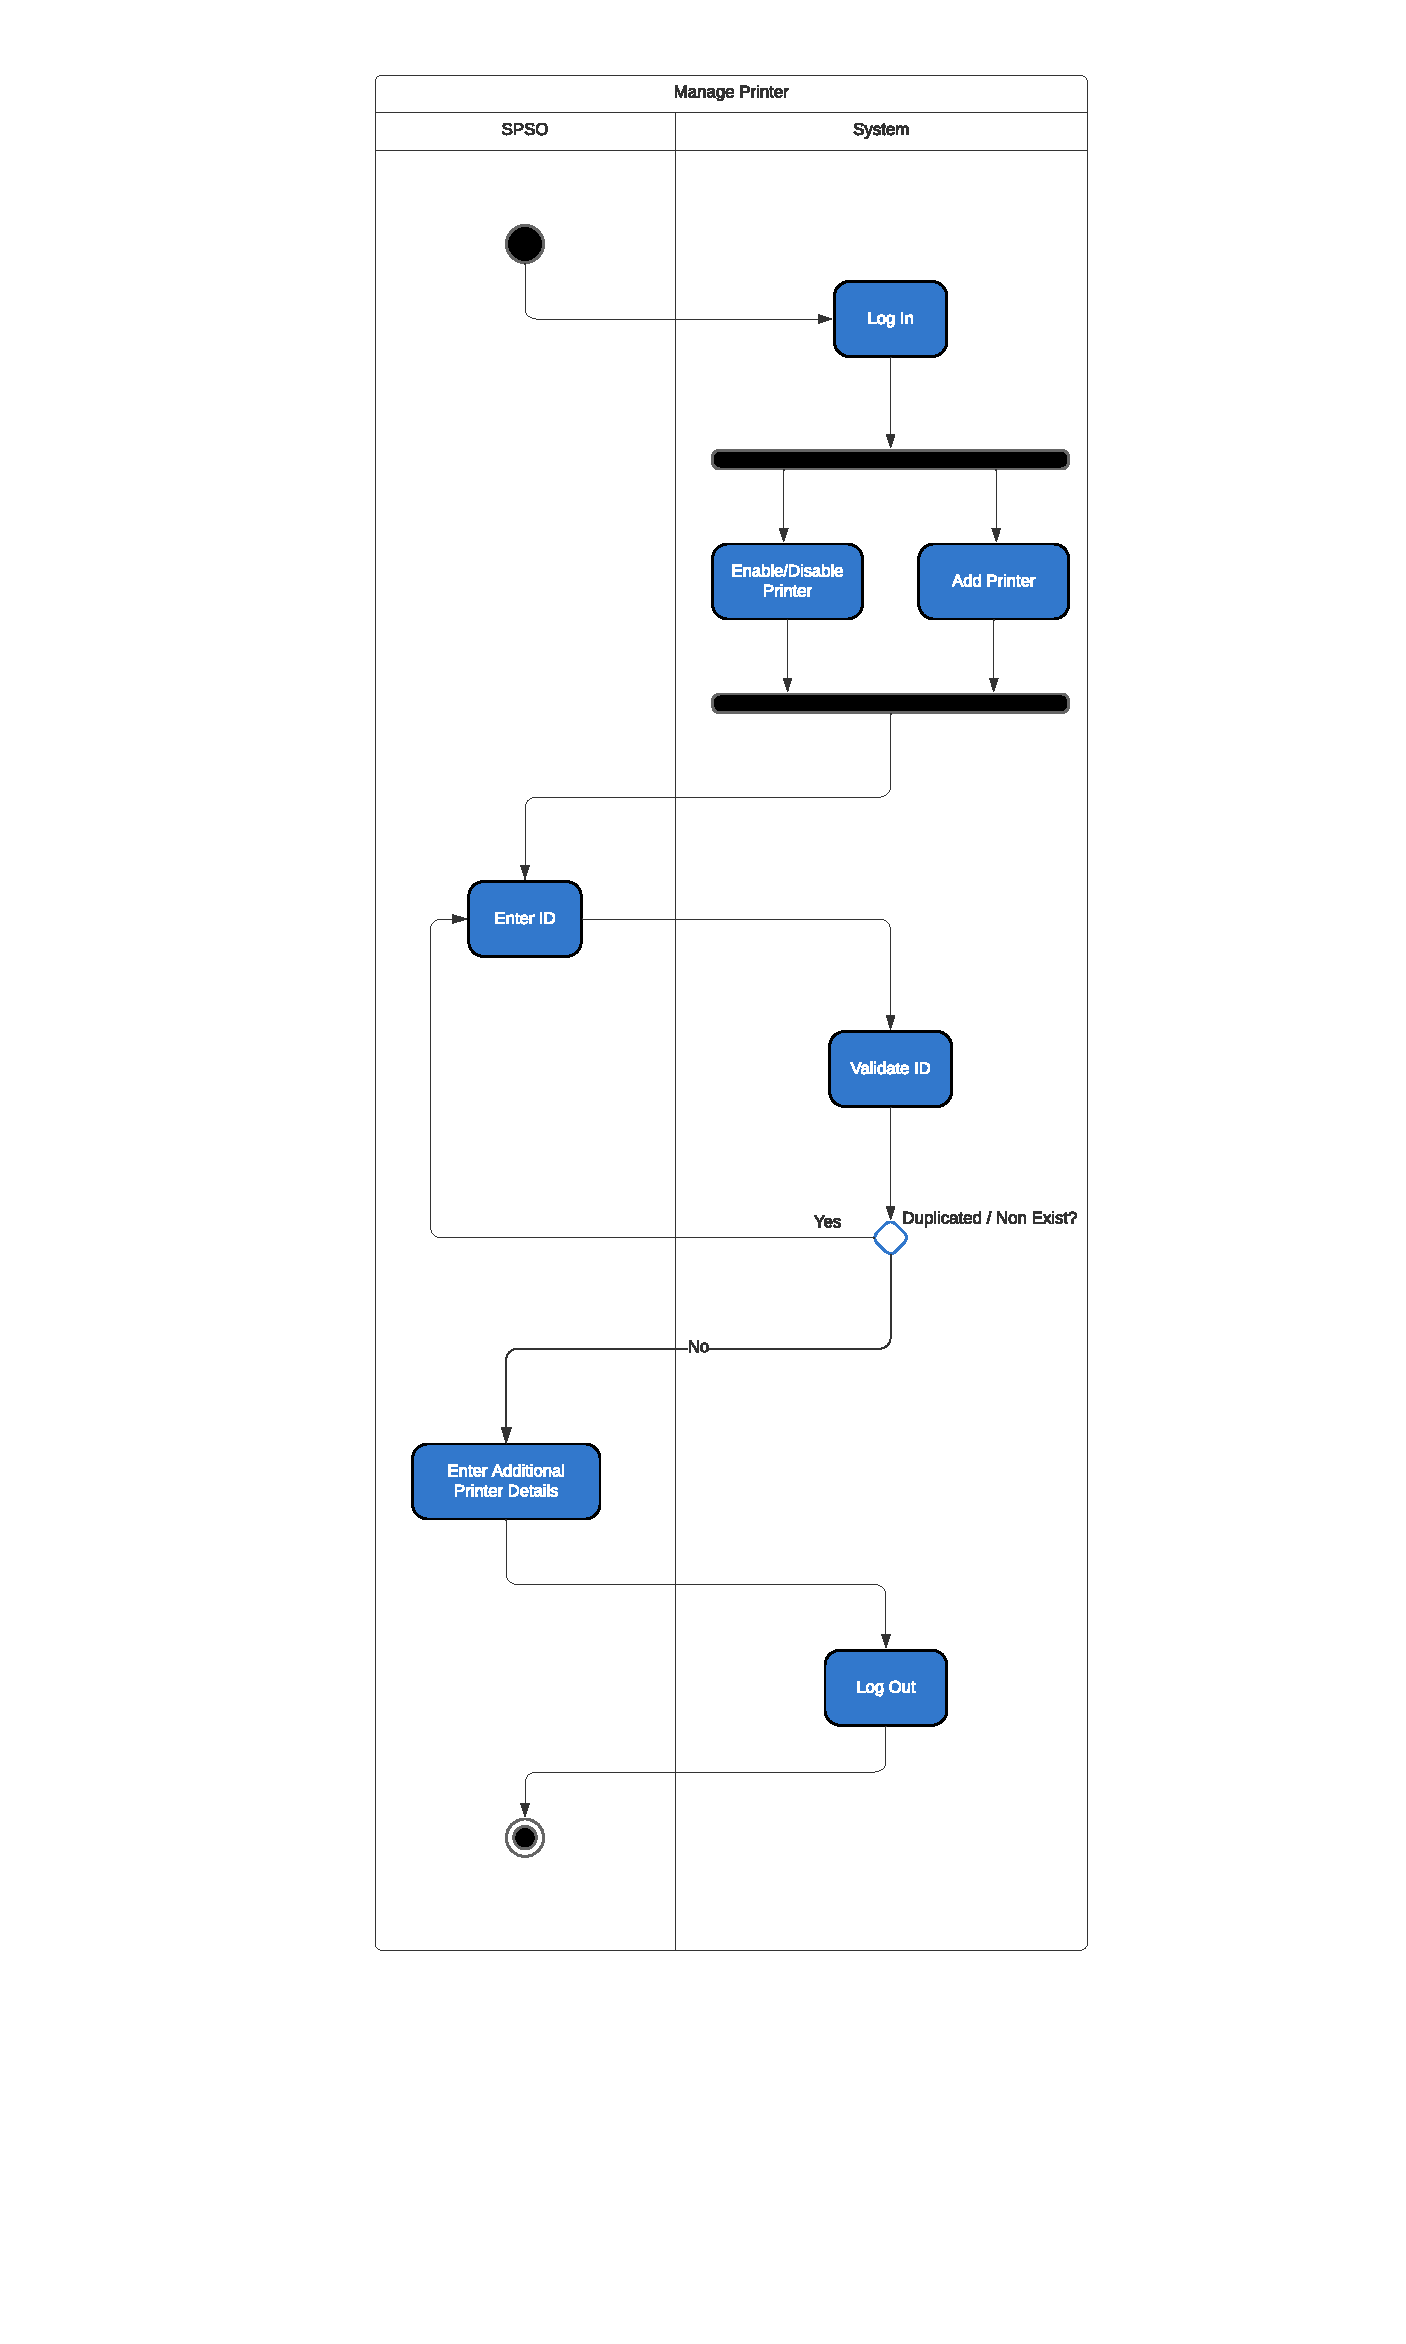
\includegraphics[scale=.45]{images/Task2/ActivityDiagrams/ManagePrinter.pdf}
    \end{center}
    \label{refhinh1}
    \end{figure}
    \end{center}

    \newpage
    \textbf{Mô tả:}
    \begin{itemize}
        \item SPSO sẽ đăng nhập vào hệ thống quản lý máy in qua dịch vụ xác thực HCMUT\_SSO, chọn vai trò (quản lý) và đăng nhập với tài khoản quản lý đã được cấp.
        \item Sau khi đăng nhập thành công, SPSO chọn chức năng quản lý (thêm máy in, bật/tắt máy in):
        \begin{itemize}
            \item Nếu chọn thêm máy in vào hệ thống, SPSO sẽ xác nhận đã có máy in vật lý được lắp đặt tại địa điểm chỉ định hay chưa.
        \end{itemize}
        \item Sau khi xác nhận chức năng, SPSO sẽ phải nhập và xác nhận ID của máy in cần được thêm/bật/tắt đang tồn tại trong hệ thống và hợp lệ, tránh trùng lặp với ID đã có sẵn trong hệ thống.
        \begin{itemize}
            \item Nếu đã chọn chức năng thêm máy in, SPSO sẽ đồng thời điền vào các thông tin của máy in (mẫu mã, địa điểm, ...).
        \end{itemize}
        \item Khi đã hoàn thành công việc quản lý máy in, SPSO sẽ đăng xuất khỏi hệ thống.
    \end{itemize}


    \newpage
    \subsubsection{Configure System}
    \begin{center}
    \begin{figure}[!htp]
    \begin{center}
     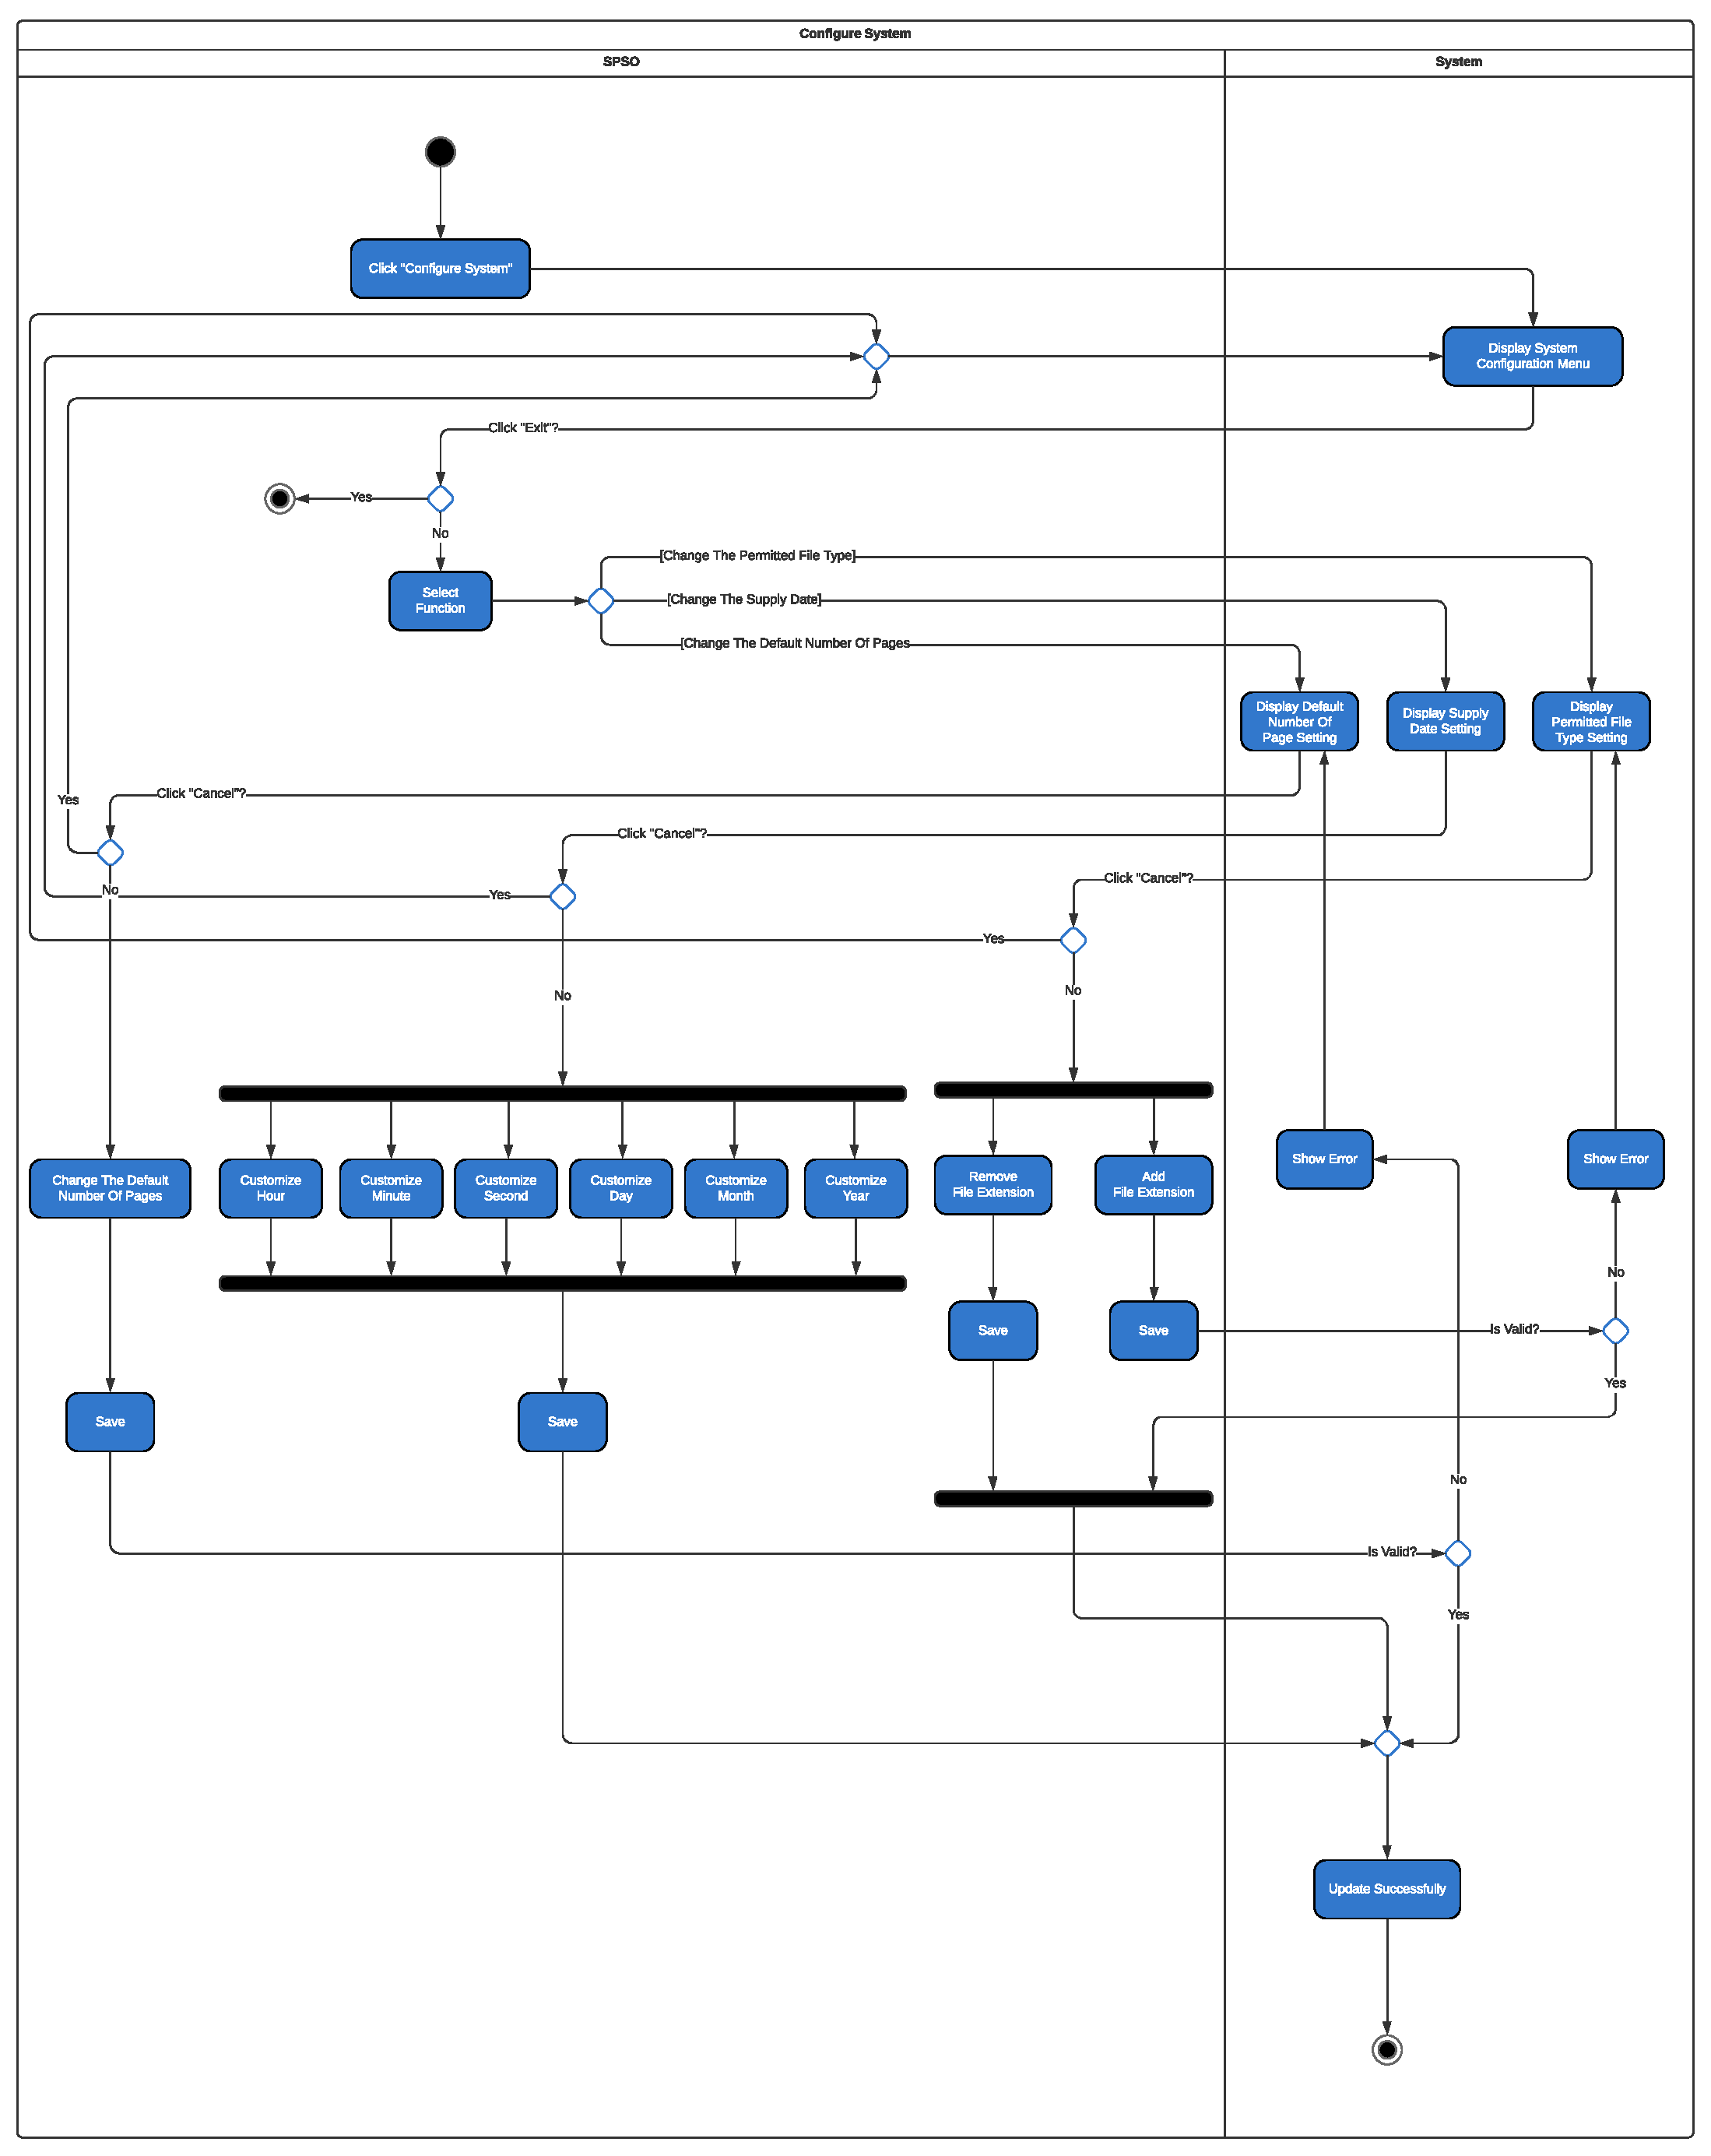
\includegraphics[scale=.4]{images/Task2/ActivityDiagrams/ConfigureSystem.pdf}
    \end{center}
    \label{refhinh1}
    \end{figure}
    \end{center}

    \newpage
    \textbf{Mô tả:}
    \begin{itemize}
        \item SPSO chọn chức năng cấu hình hệ thống trong trang chính, trang tùy chỉnh các cấu hình của hệ thống sẽ hiện ra.\\
        \item SPSO chọn một trong ba chức năng để tiến hành tùy chỉnh.\\
        \begin{itemize}
            \item Nếu SPSO chọn thay đổi số giấy in mặc định, SPSO có thể thay đổi số giấy in mặc định bằng một con số bất kì, con số này phải là số nguyên dương. Khi lưu, hệ thống sẽ kiểm tra sự hợp lệ của số giấy in mặc định mới để xác nhận đã lưu thành công.\\
            \item Nếu SPSO chọn thay đổi thời điểm cung cấp giấy in, SPSO có thể tùy chỉnh các thông số như ngày, tháng, năm, giờ, phút, giây. Các thông số này sẽ được thay đổi bằng các drop down list. Sau đó SPSO cần bấm lưu để thực hiện cập nhật thông số.
            \item Đối với chức năng chỉnh sửa các định dạng tệp tin được cho phép, SPSO có thể thêm định dạng mới hoặc xóa bớt các định dạng đã có sẵn.
        \end{itemize}
    \end{itemize}


    \newpage
    \subsubsection{Log In}
    \begin{center}
    \begin{figure}[!htp]
    \begin{center}
     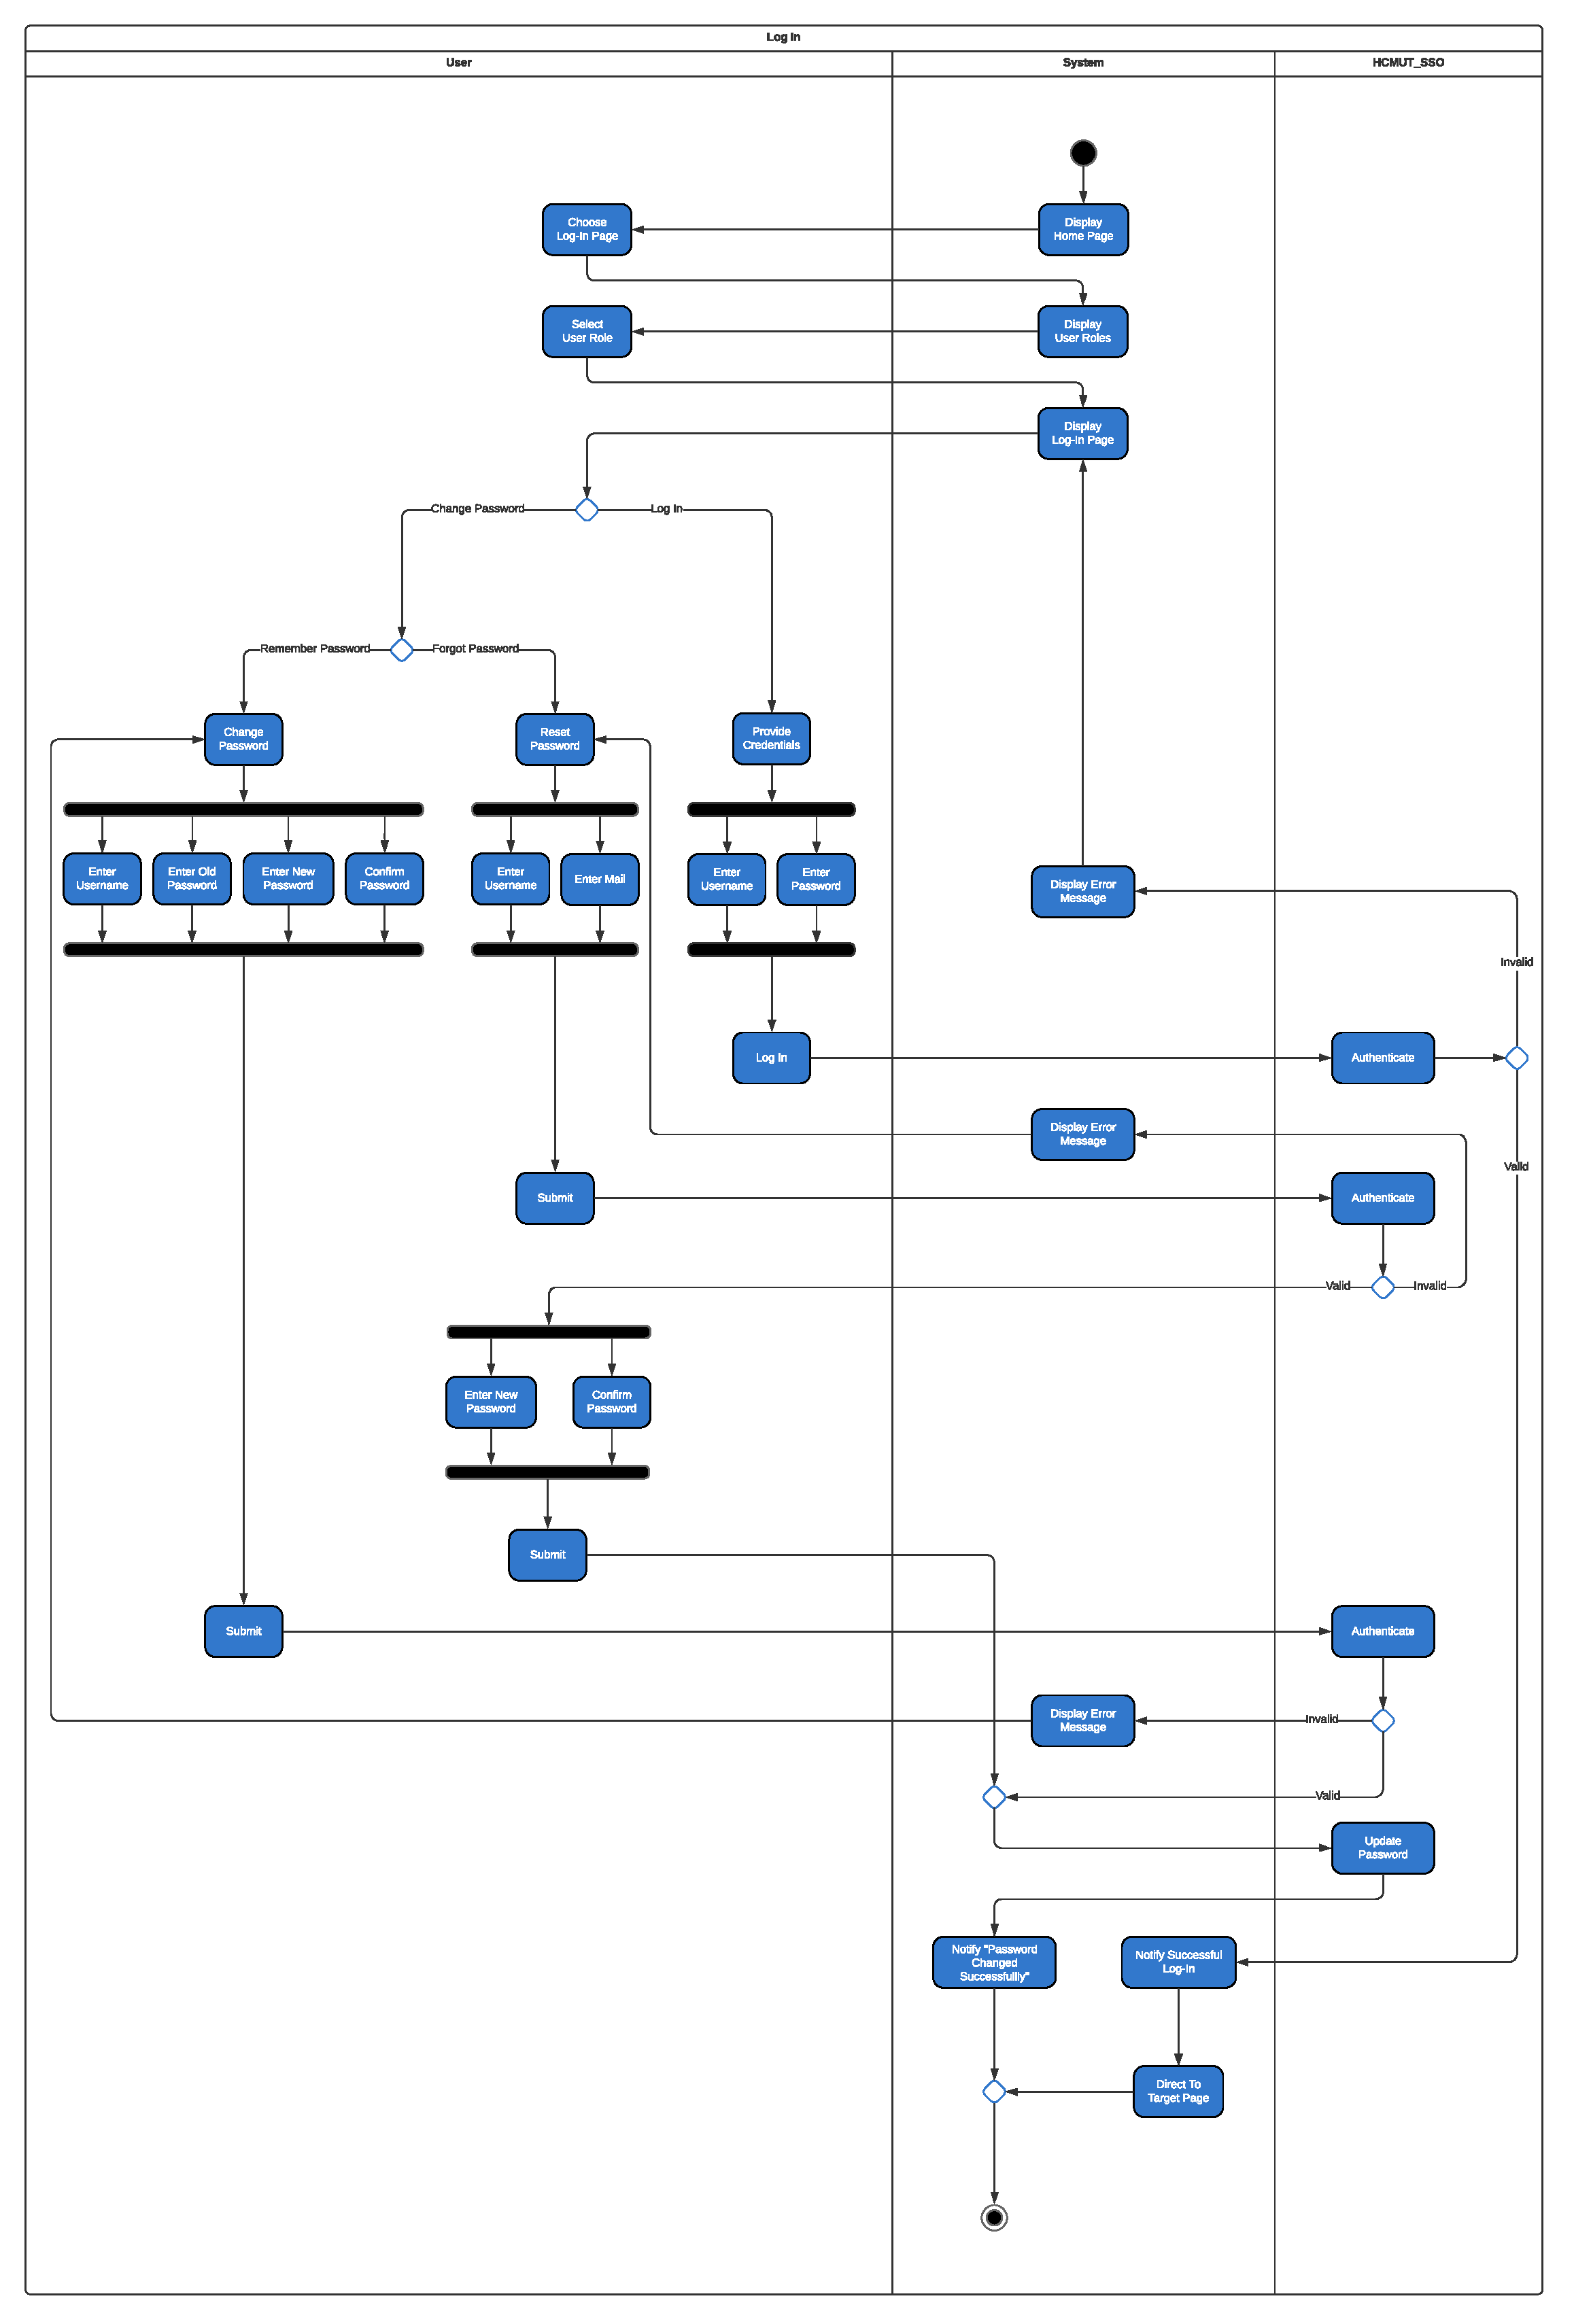
\includegraphics[scale=.34]{images/Task2/ActivityDiagrams/LogIn.pdf}
    \end{center}
    \label{refhinh1}
    \end{figure}
    \end{center}

    \newpage
    \textbf{Mô tả:}
    \begin{itemize}
    \item Người dùng thông qua giao diện để gửi thông tin đăng nhập (username + password) đến hệ thống.
    \item Sau khi nhận được thông tin đăng nhập mà người dùng cung cấp, HCMUT\_SSO sẽ tiến hành xác thực:
        \begin{itemize}
            \item Nếu thông tin đăng nhập được xác nhận thành công (Valid), giao diện sẽ chuyển đến trang sử dụng dịch vụ in (Target Page) để người dùng có thể tiếp tục các lựa chọn trải nghiệm.
            \item Nếu thông tin đăng nhập không xác nhận thành công (Invalid), hệ thống sẽ hiển thị thông báo lỗi và giao diện sẽ chuyển về trang đăng nhập (Log-In Page) để người dùng có thể cung cấp lại thông tin đăng nhập.
        \end{itemize}
    \item Ngoài ra, người dùng có thể thay đổi mật khẩu cho tài khoản của mình:
        \begin{itemize}
            \item Trường hợp người dùng không nhớ mật khẩu hiện tại, người dùng có một sự lựa chọn duy nhất là đổi mật khẩu thông qua mail - Reset Password (username, mail).
            \item Trường hợp người dùng vẫn nhớ mật khẩu hiện tại, người dùng sẽ có thêm một sự lựa chọn khác là đổi mật khẩu thông qua mật khẩu cũ - Change Password (user name , old password).
        \end{itemize}
    \end{itemize}
        \newpage
    \subsection{Task 2.2: Sequence diagrams}
    \subsubsection{Request For Printing Service}
    \begin{center}
    \begin{figure}[!htp]
    \begin{center}
     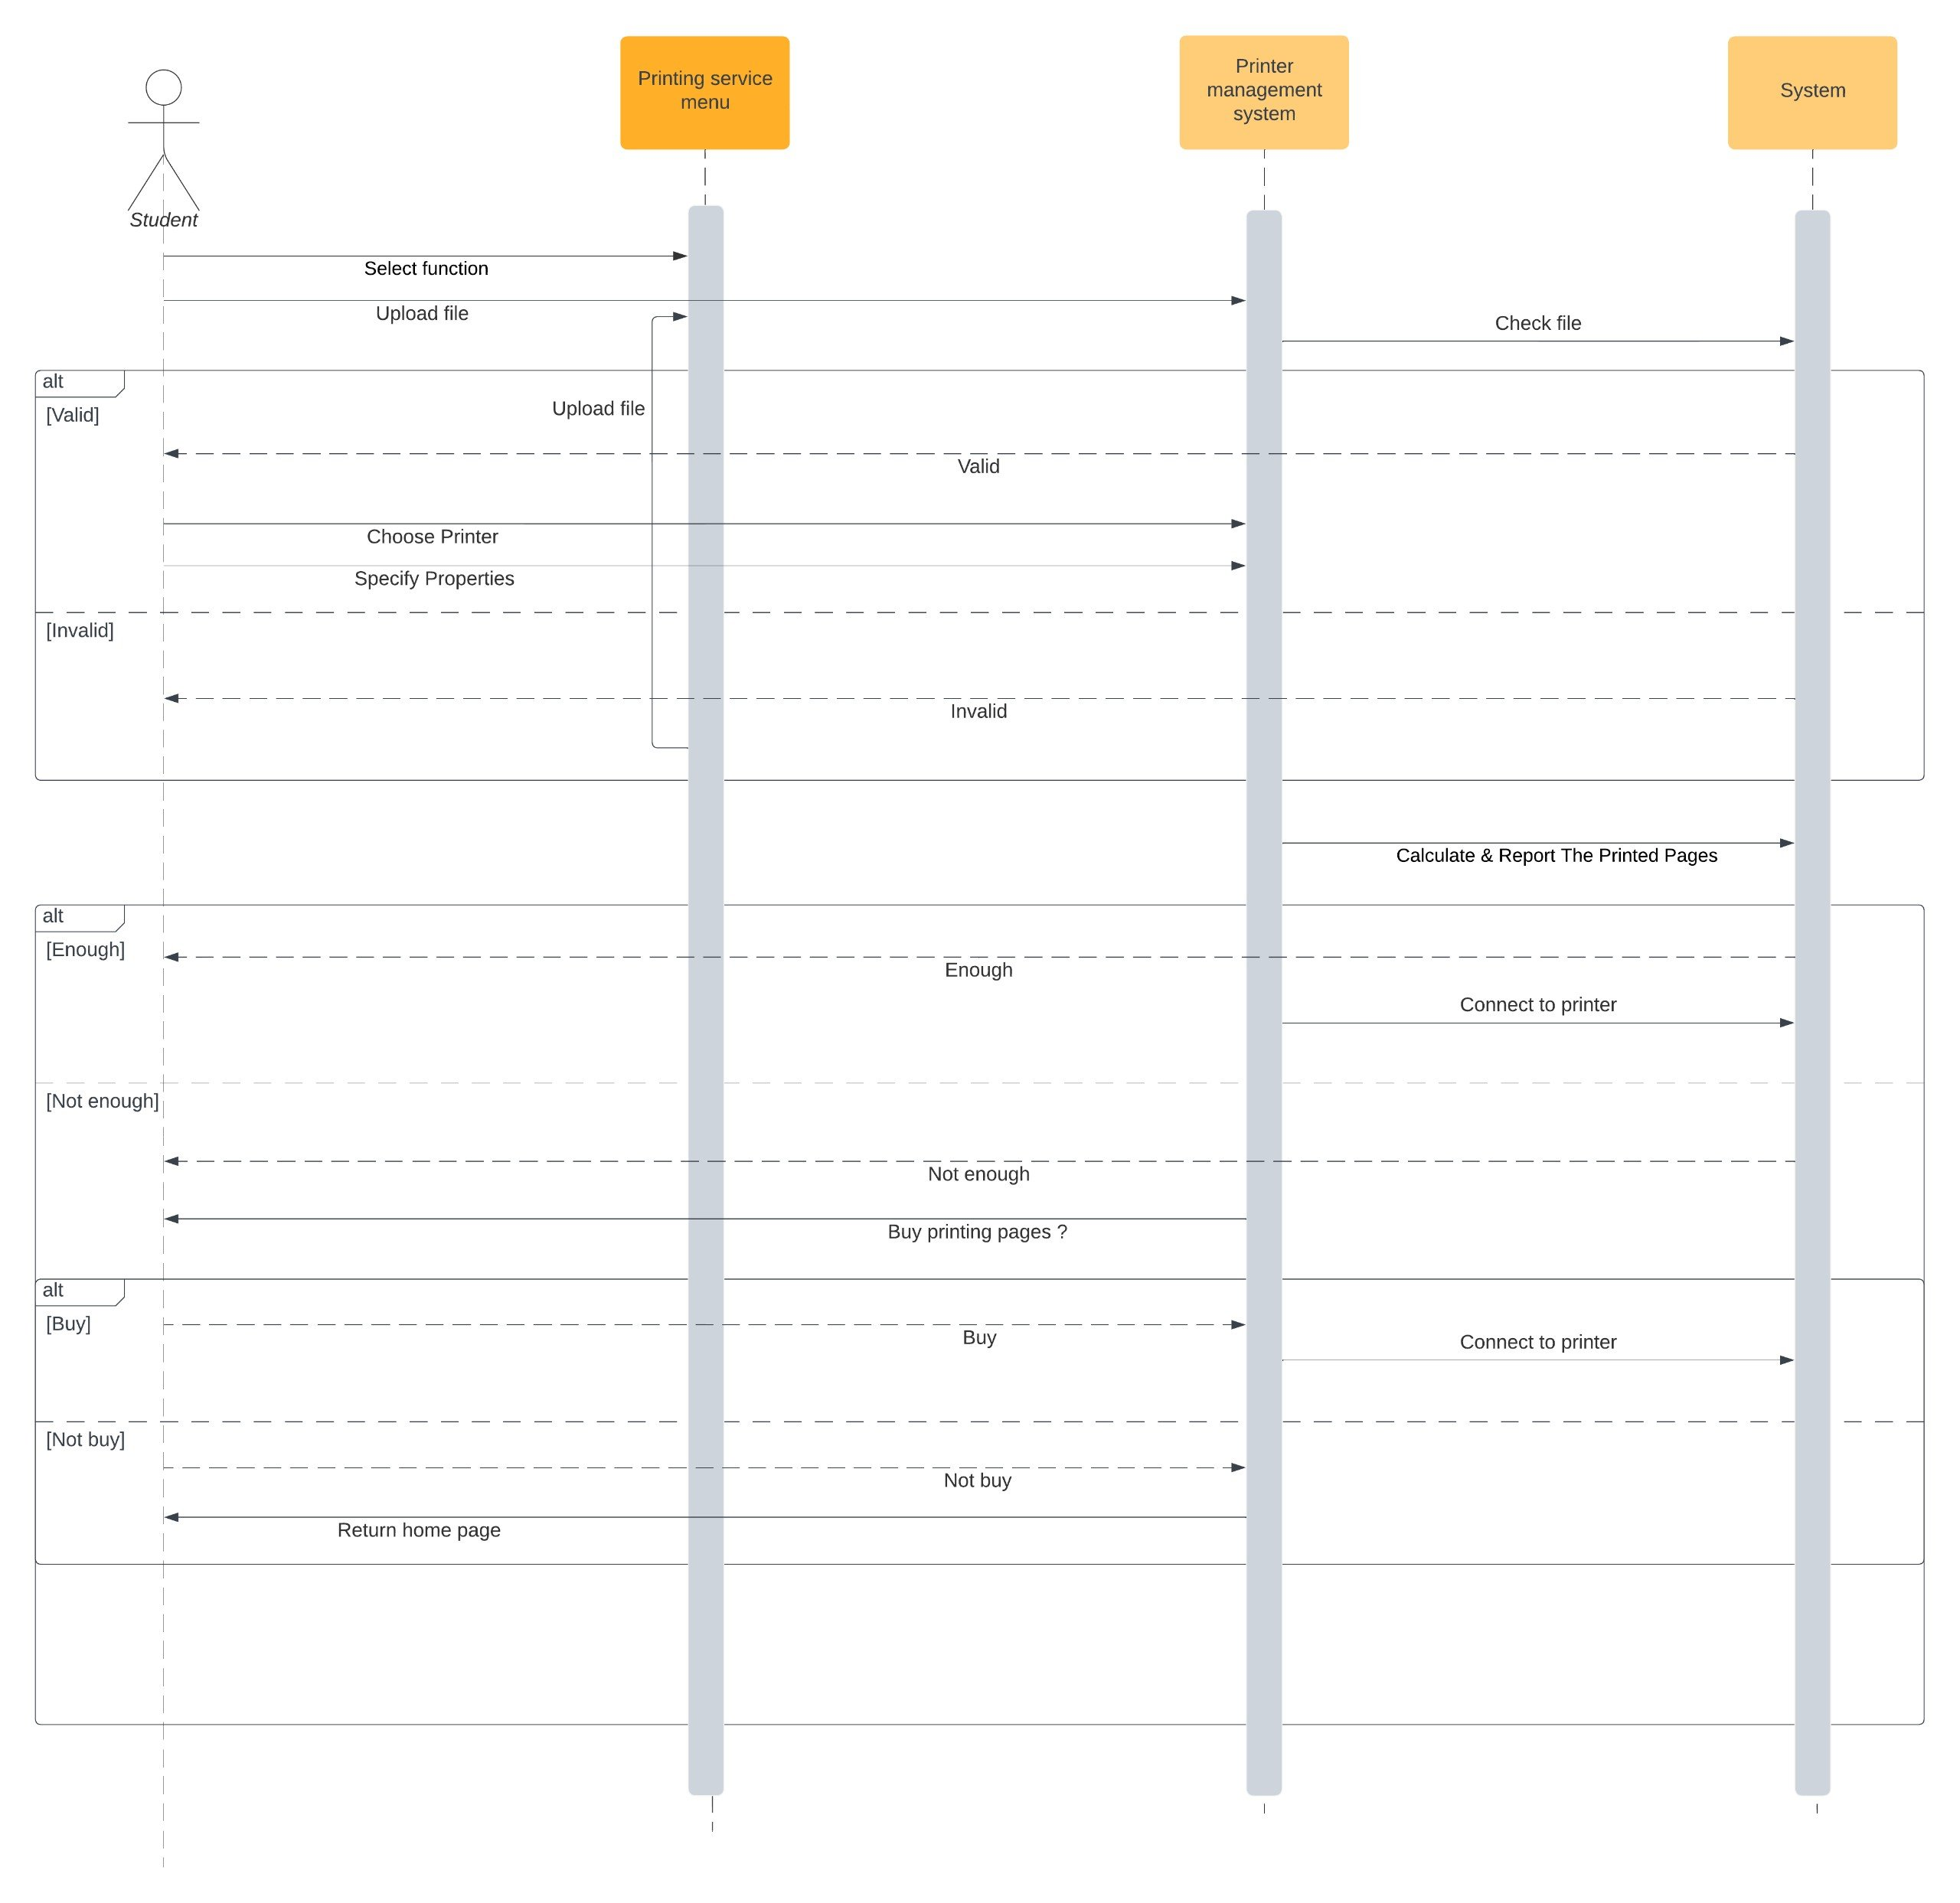
\includegraphics[scale=.19]{images/Task2/SequenceDiagrams/RequestForPrintingService.jpg}
    \end{center}
    \label{refhinh1}
    \end{figure}
    \end{center}

    \newpage
    \textbf{Mô tả:}
    \begin{itemize}
        \item Người dùng tiến hành tải file in lên hệ thống quản lý.
        \item Hệ thống sẽ tự động kiểm tra tính hợp lệ và hiển thị thông báo cho người dùng:
        \begin{itemize}
            \item Nếu file hợp lệ người dùng được phép chọn máy in và cấu hình các thuộc tính in.
            \item Nếu file không hợp lệ hệ thống đưa người dùng trở lại bước tải file ban đầu và tải lên lại file mới.
        \end{itemize}
        \item Tiếp đó hệ thống sẽ tính toán lại số lượng trang được in còn lại của sinh viên và báo cáo lại cho người dùng:
        \begin{itemize}
            \item Nếu đủ số trang hệ thống sẽ tiến hành in cho sinh viên.
            \item Nếu thiếu số trang để in người dùng được chuyển tới chức năng mua trang in:
            \begin{itemize}
                \item Nếu sinh viên mua đủ hoặc hơn số trang để in hệ thống sẽ tiến hành in.
                \item Nếu sinh viên chọn không mua hệ thống sẽ đem sinh viên về trang chủ
            \end{itemize}
        \end{itemize}
    \end{itemize}

    \newpage
    \subsubsection{Make Online Payment}
    \begin{center}
    \begin{figure}[!htp]
    \begin{center}
     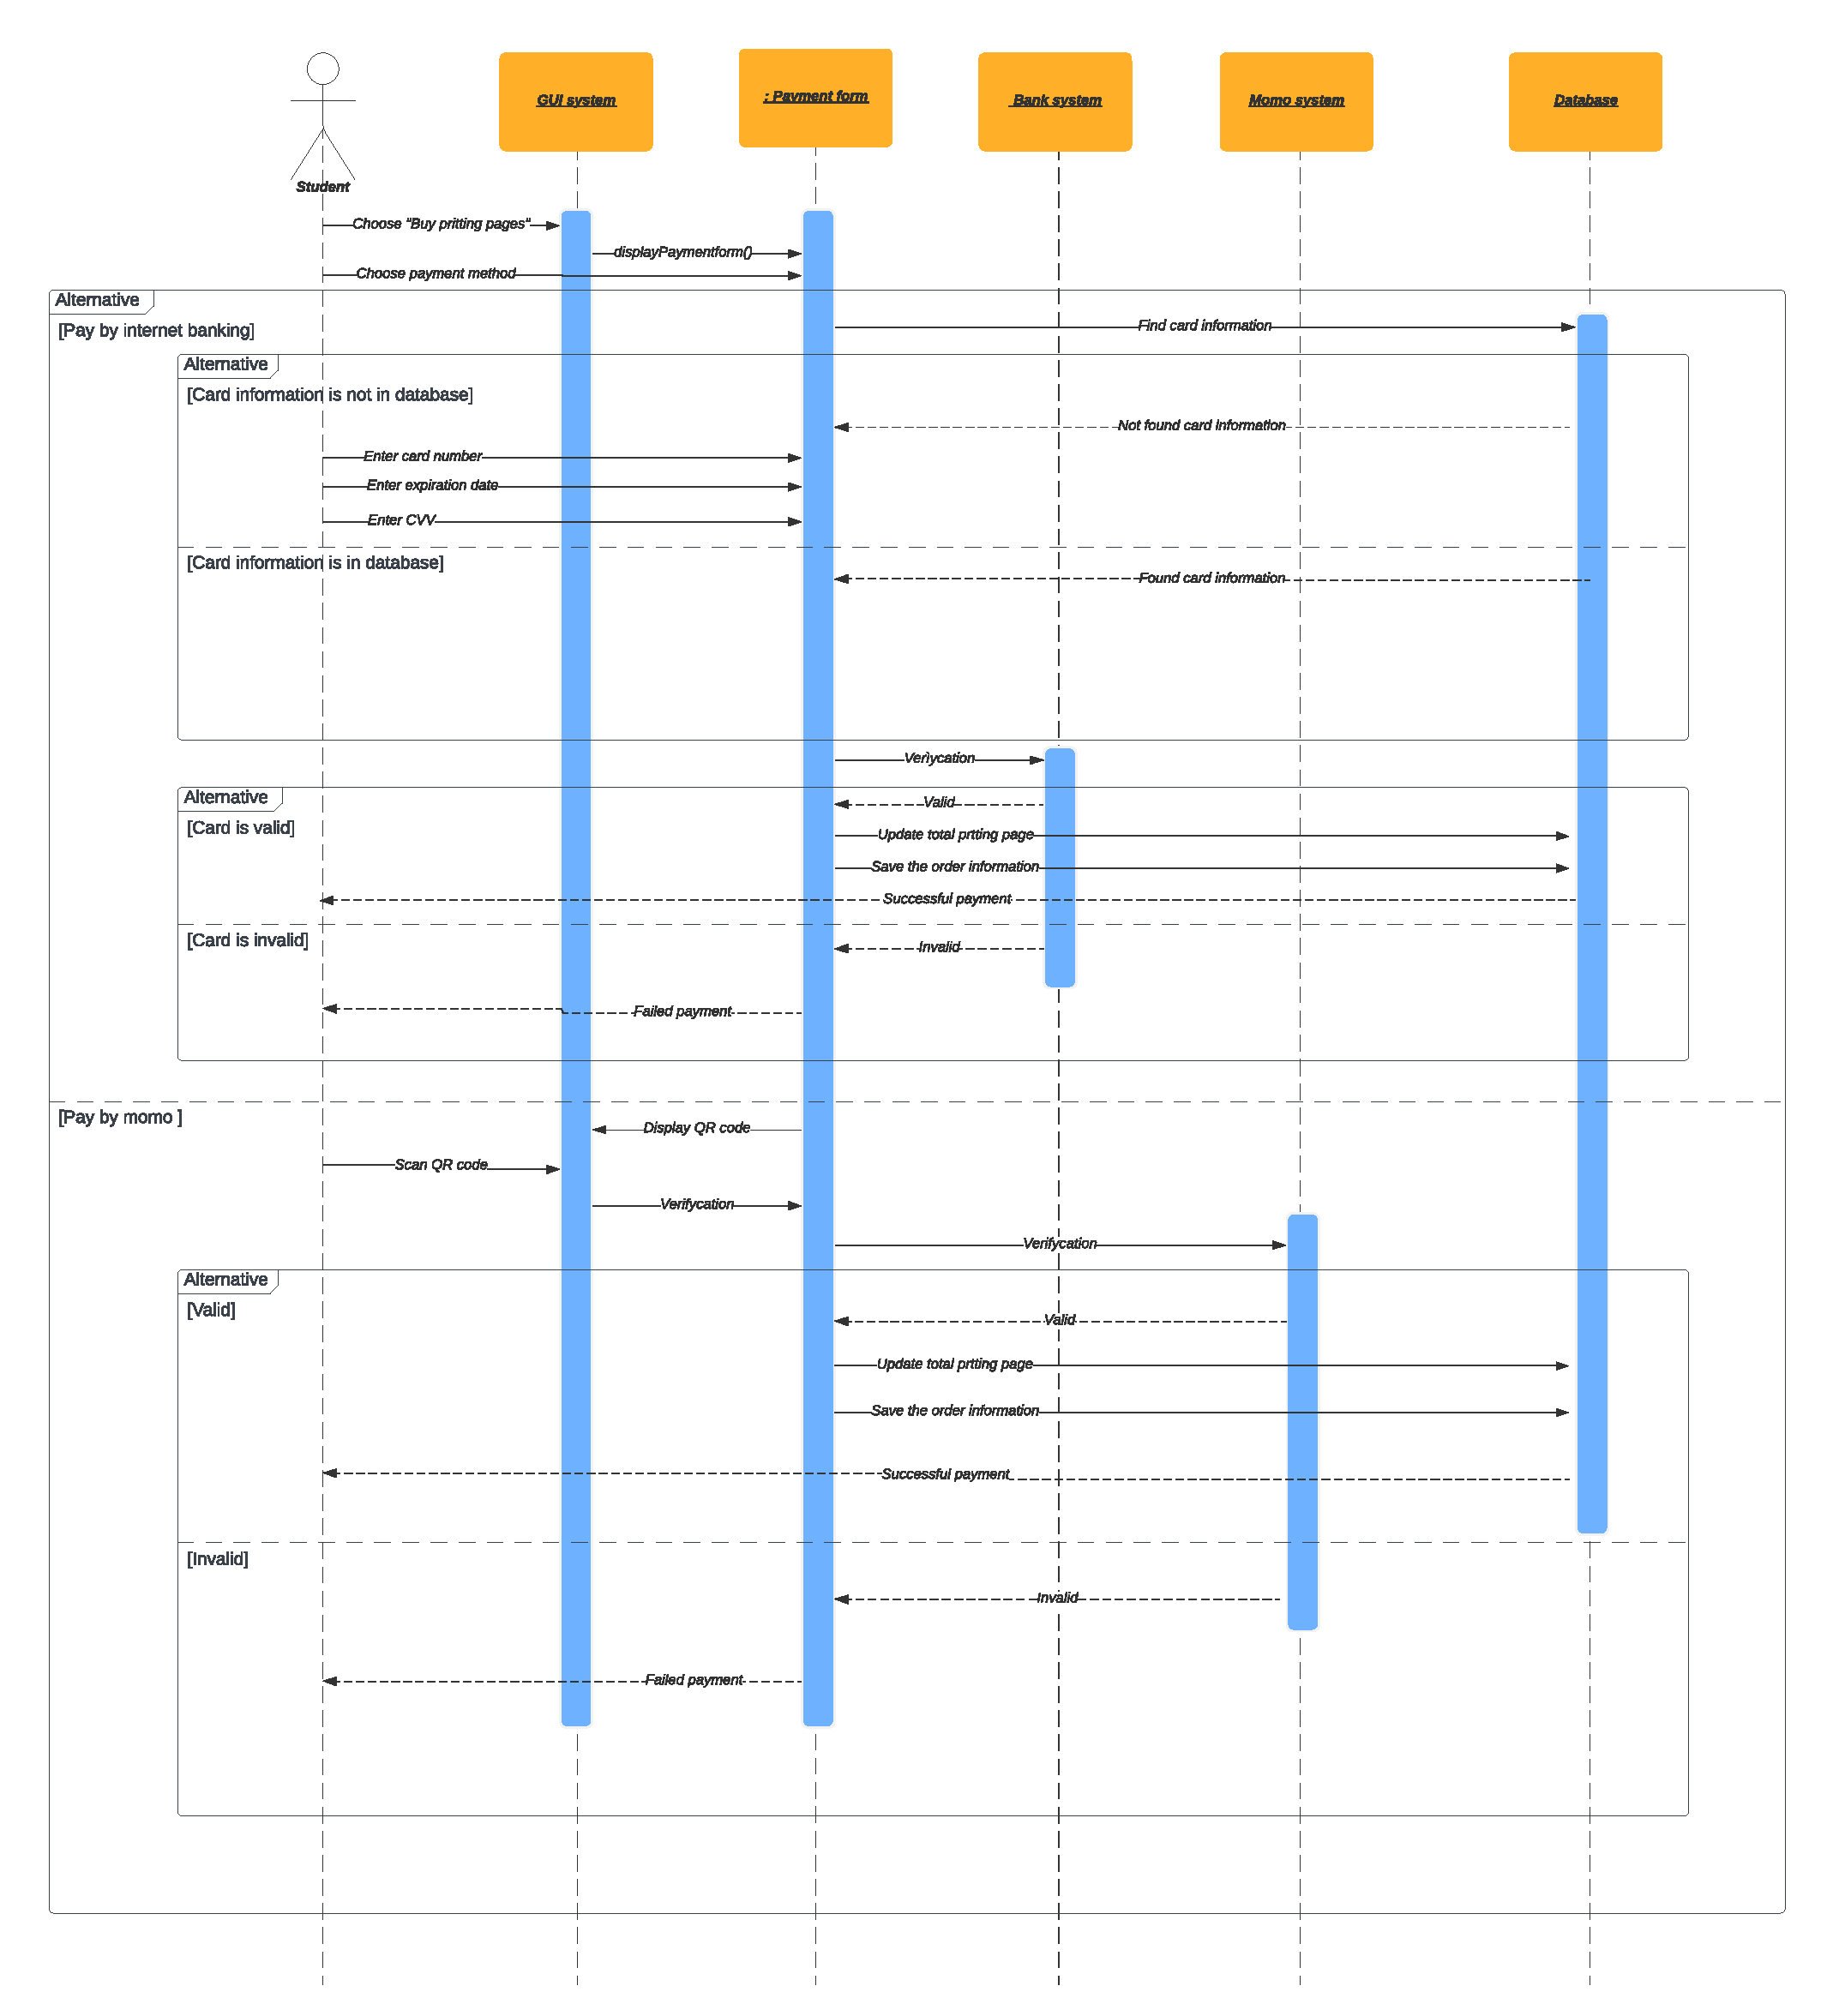
\includegraphics[scale=0.45]{images/Task2/SequenceDiagrams/PaymentSequence.pdf}
    \end{center}
    \label{refhinh1}
    \end{figure}
    \end{center}
        \newpage
    \textbf{Mô tả:}
\begin{itemize}
        \item Sinh viên chọn dịch vụ mua giấy in để tiến hành mua thêm giấy in
        \item Sau khi đăng nhập thành công, sinh viên chọn chức năng "Mua giấy in", sau đó hệ thống sẽ hiển thị giao diện mua giấy in để sinh viên có thể chọn số lượng giấy in mình cần mua.
        \item Hệ thống dựa vào số lượng giấy in mà sinh viên chọn cùng với giá của giấy in tại thời điểm sinh viên mua mà tính toán ra số tiền cần trả để sinh viên kiểm tra và xác nhận.
        \item Sau khi xác nhận giá thì sinh viên sẽ chọn 1 trong 2 phương thức thanh toán là qua visacard hay là ví điện tử momo
        \begin{itemize}
            \item Nếu sinh viên chọn thanh toán qua visacard thì cần phải nhập thông tin bao gốm số thẻ, ngày hết hạn và mã bảo vệ. Hệ thống sẽ gửi API đến ngân hàng để xác nhận thông tin thanh toán.
            \item Nếu sinh viên chọn thanh toán qua momo thì hệ thống sẽ hiển thị mã QR, sinh viên thực hiện quét mã và hệ thống sẽ gửi API đến ví điện tử momo để xác nhận thông tin thanh toán.
        \end{itemize}
        \item Trong cả 2 trường hợp nếu thanh toán thành công thì sẽ cập nhật số lượng giấy in của sinh viên, lưu lại hóa đơn thanh toán đồng thời hiển thị ra màn hình để sinh viên xác nhận.
        \item Nếu việc thanh toán thất bại thì hệ thống sẽ hiển thị thông báo lỗi và quay trở về bước thanh toán trước đó.
    \end{itemize}


    \newpage
    \subsubsection{Manage Printers}
    \begin{center}
    \begin{figure}[!htp]
    \begin{center}
     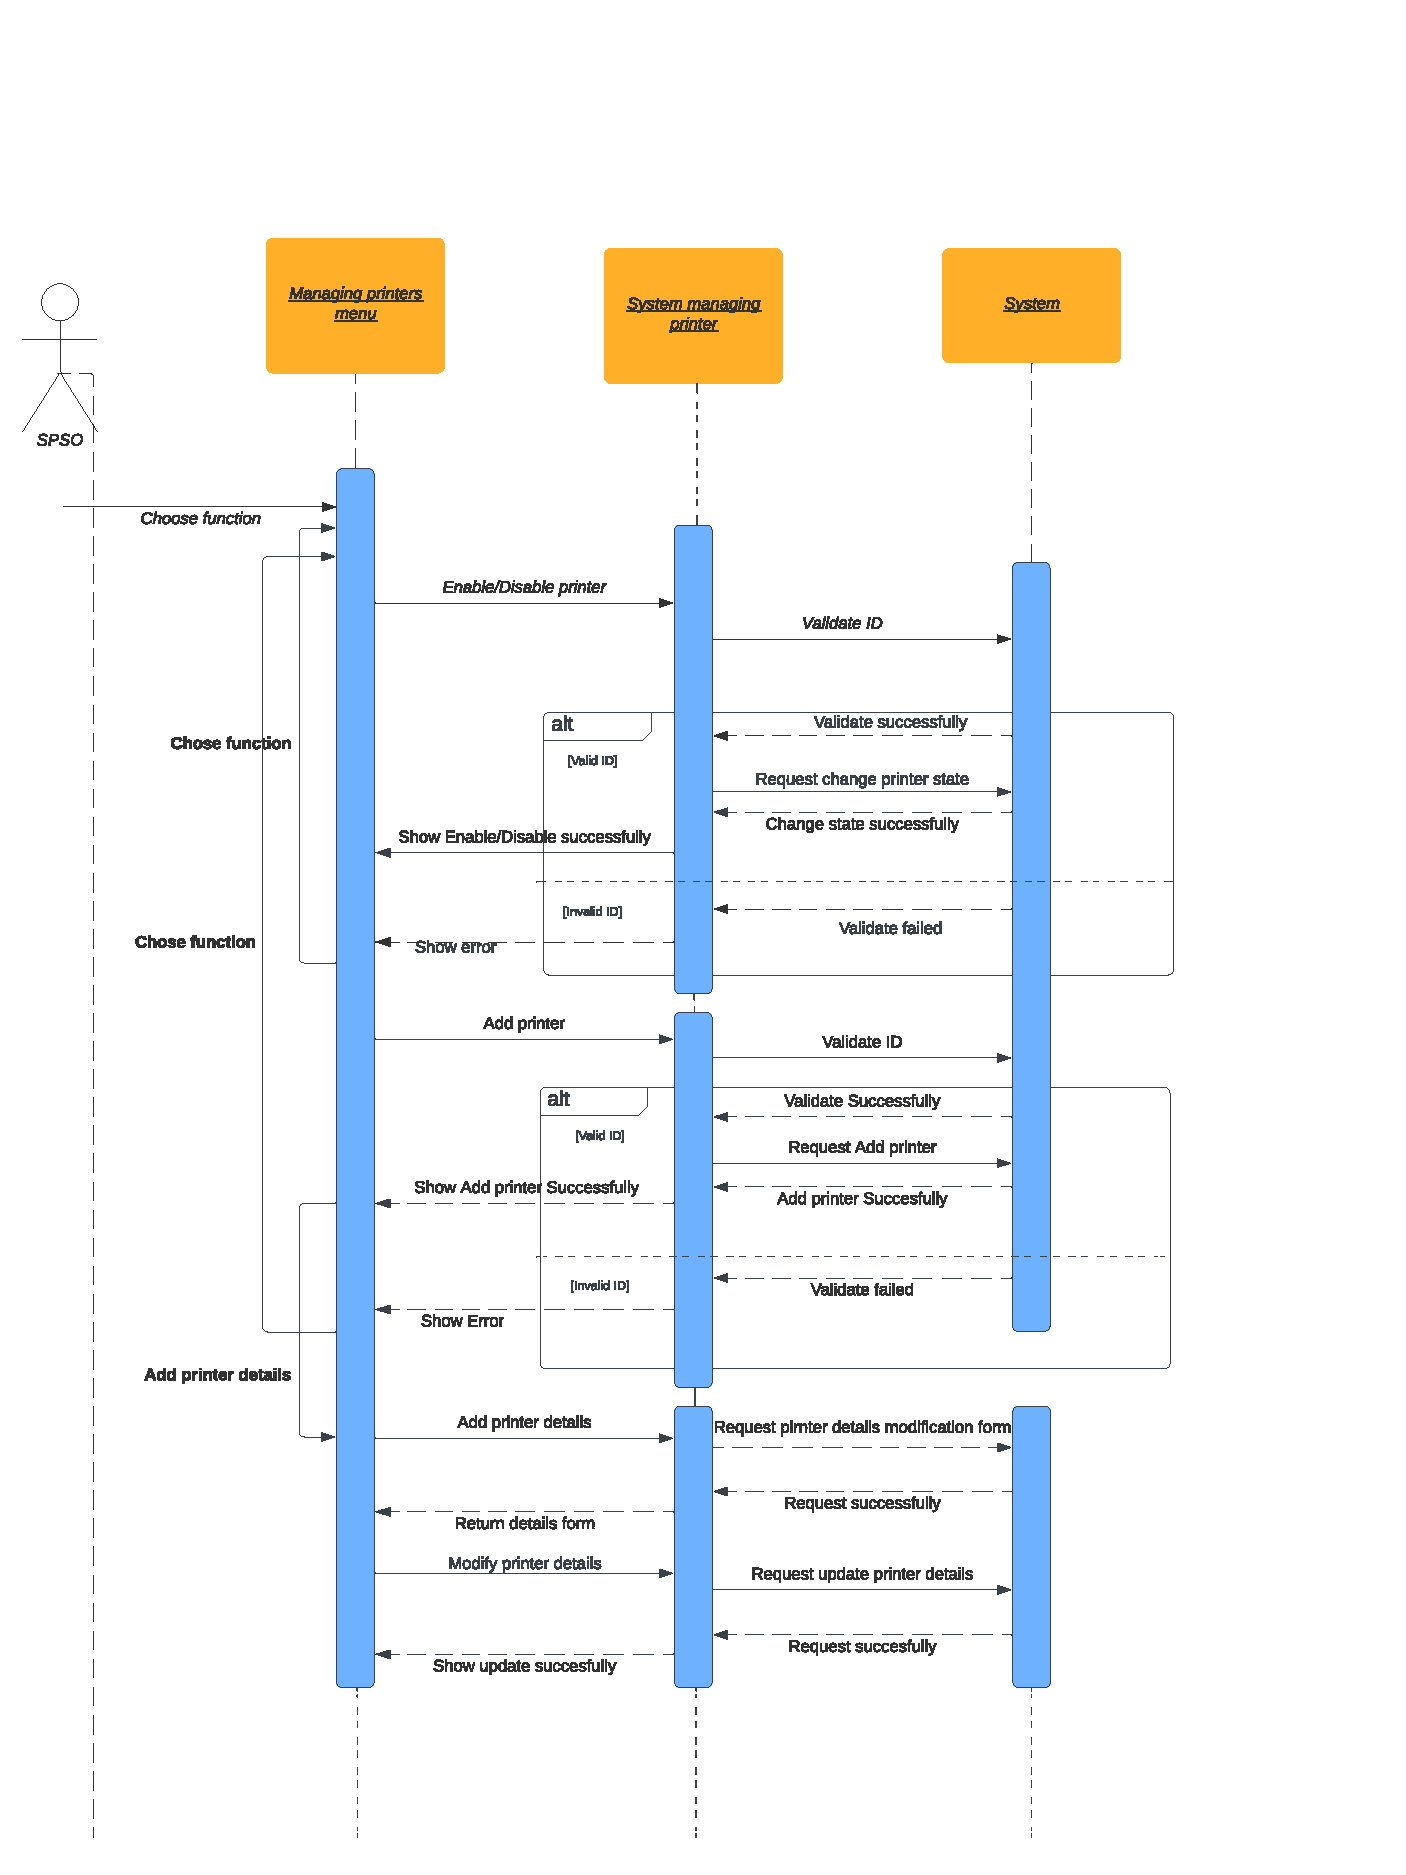
\includegraphics[scale=.6]{images/Task2/SequenceDiagrams/ManagePrinter.pdf}
    \end{center}
    \label{refhinh1}
    \end{figure}
    \end{center}

    \textbf{Mô tả:}
    Sau khi đăng nhập, SPSO sẽ vào giao diện để dành riêng cho SPSO, sau đó SPSO có thể chọn vào Quản lý máy in. \\

    Tại trang quản lý máy in, SPSO có thể lựa chọn giữa chức năng Thêm máy in và Bật / Tắt máy in. 
    \begin{itemize}
        \item Sau khi chọn Bật / Tắt máy in, SPSO nhập ID cho máy in cần bật hoặc tắt. Nếu ID hợp lệ, hệ thống quản lý máy in sẽ gửi request cho hệ thống in ấn để thay đổi trạng thái máy in theo yêu cầu, rồi trả về thống báo đã thay đổi cho SPSO. Nếu nhập sai ID hoặc ID không hợp lệ thì hệ thống sẽ báo lỗi sai ID và trả SPSO về trang quản lý máy in.
        \item Nếu chọn thêm máy in, SPSO nhập ID cho máy in muốn được thêm mới. Nếu ID hợp lệ, hệ thống quản lý máy in sẽ gửi request cho hệ thống in ấn để cho phép SPSO nhập tiếp các thông tin còn lại của máy in (tên, mẫu mã, ...) rồi gửi các thông tin đó đến hệ thống. Sau đó, hệ thống sẽ cập nhật thông tin máy in giống như đã nhập và trả về thống báo đã thêm thành công.
    \end{itemize}


    \newpage
    \subsubsection{Configure System}
    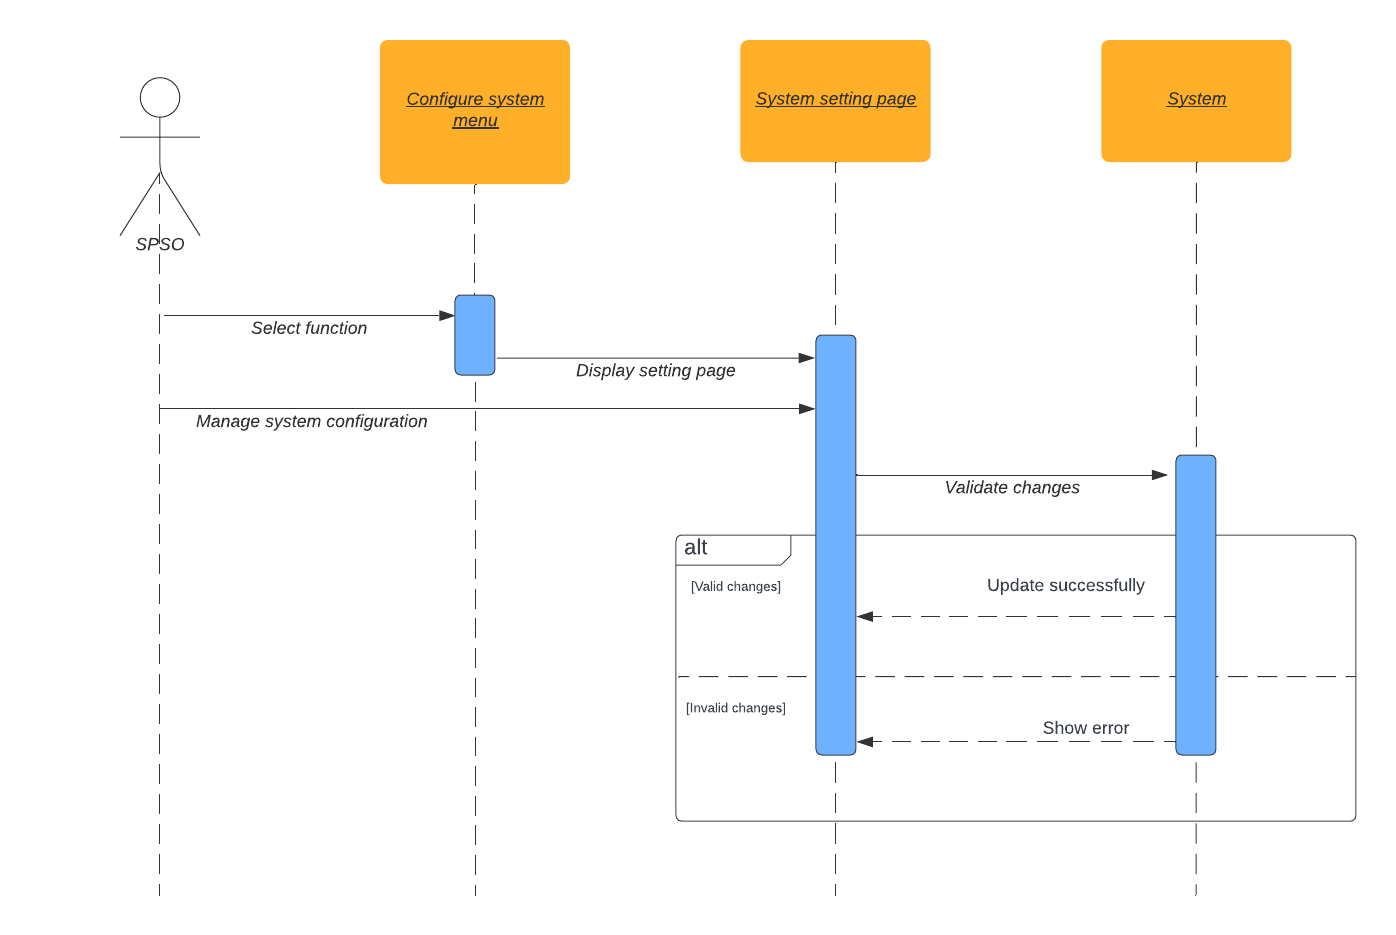
\includegraphics[width=\textwidth]{images/Task2/SequenceDiagrams/ConfigureSystem_SequenceDiagram.png}
    \textbf{Mô tả:}
    Biểu đồ mô tả sự tương tác của SPSO với các objects khác là Configure system menu, System setting page và system. Vai trò của SPSO là chọn chức năng cần tùy chỉnh trong Configure system menu và tiến hành tùy chỉnh trong system setting page. Nhìn qua biểu đồ, ta có thể thấy thời gian hoạt động của System setting page là nhiều nhất, đúng với vai trò chính của chức năng tùy chỉnh cấu hình hệ thống.\\

    \newpage
    \subsubsection{Log In}
    \begin{center}
    \begin{figure}[!htp]
    \begin{center}
     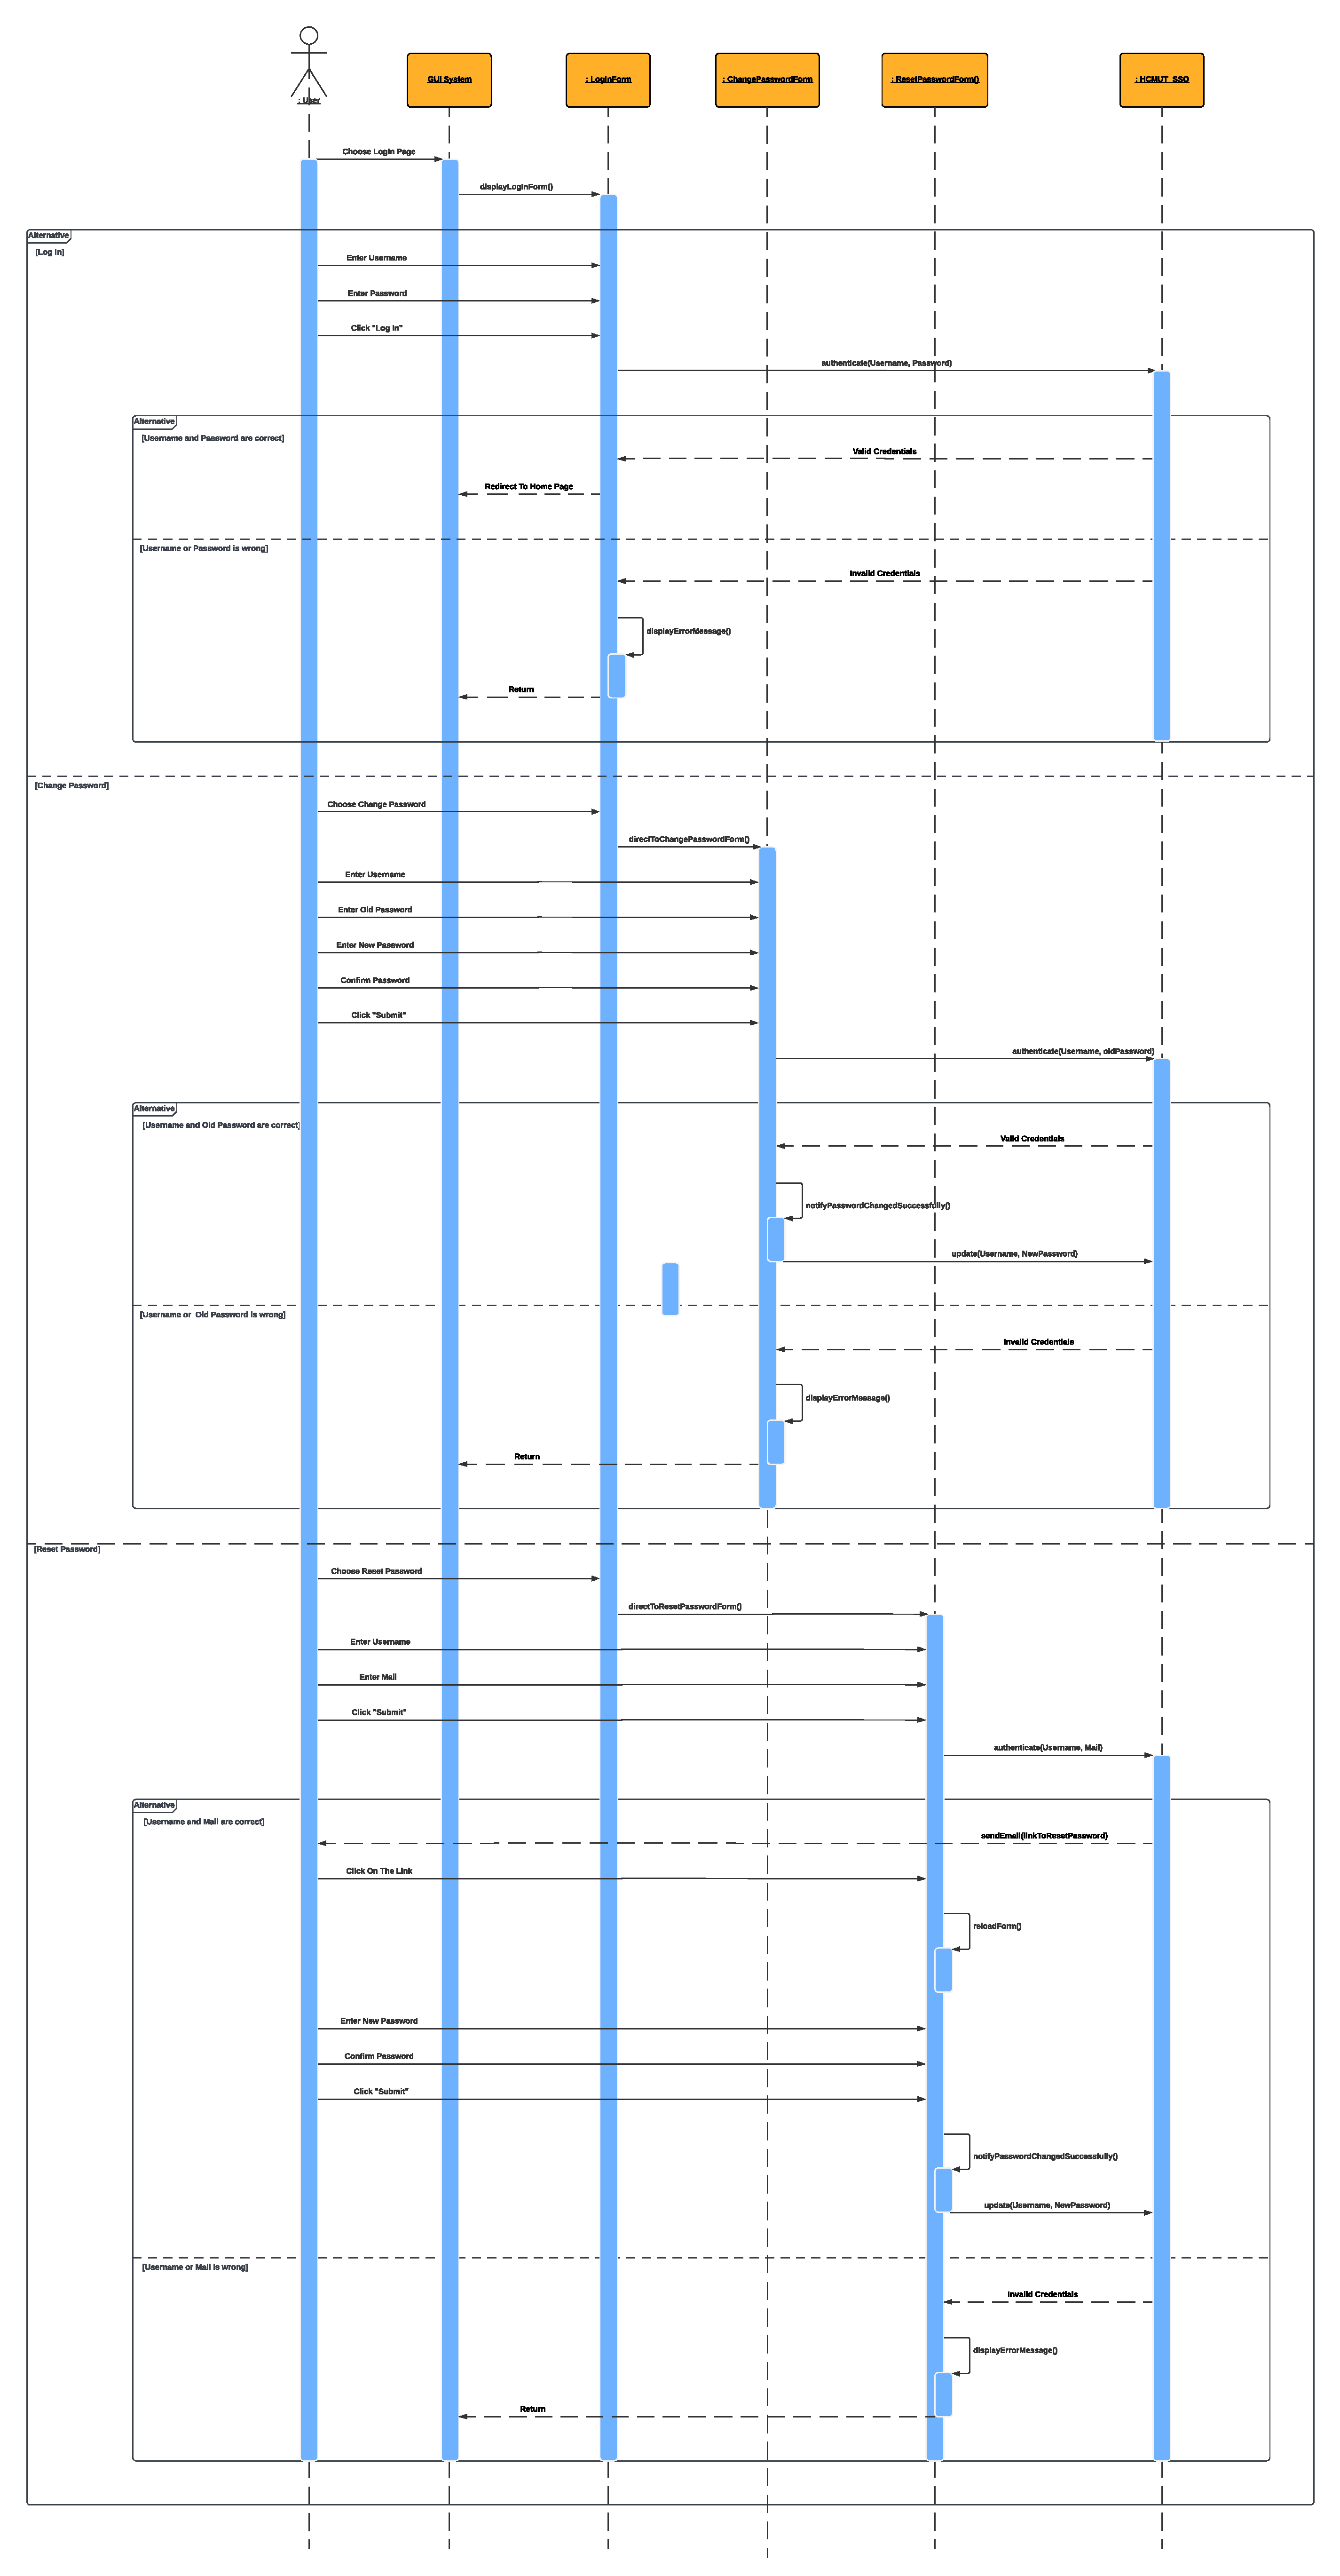
\includegraphics[scale=.21]{images/Task2/SequenceDiagrams/LogIn.pdf}
    \end{center}
    \label{refhinh1}
    \end{figure}
    \end{center}

    \textbf{Mô tả:}\\
    
        Tại giao diện đăng nhập, người dùng nhập thông tin (username, password) và chọn "Log In" để gửi yêu cầu đăng nhập.\\
        
        Dịch vụ xác thực HCMUT\_SSO sẽ tiến hành xác thực thông tin đăng nhập mà người dùng cung cấp.
        \begin{itemize}
            \item Thông tin xác thực hợp lệ: Người dùng sẽ được điều hướng tới giao diện trang chủ của trang web để tiếp tục sử dụng các dịch vụ khác.
            \item Thông tin xác thực không hợp lệ: Tại giao diện đăng nhập, một thông báo về sai thông tin đăng nhập sẽ được hiển thị.
        \end{itemize}
        
        Tại giao diện đăng nhập, người dùng còn có 2 tuỳ chọn khác:
        \begin{itemize}
            \item Thay đổi mật khẩu: 
            \begin{itemize}
                \item Khi người dùng chọn "Change Password", trang web sẽ điều hướng tới trang Change Password. Tại đây người dùng cần cung cấp các thông tin (username, old password, new password, comfirm password) và chọn "Submit" để gửi yêu cầu thay đổi mật khẩu.
                \item Dịch vụ xác thực HCMUT\_SSO sẽ tiến hành xác thực thông tin đăng nhập mà người dùng cung cấp:
                \begin{itemize}
                    \item Thông tin xác thực hợp lệ: Mật khẩu mới sẽ được cập nhật. Tại giao diện thay đổi mật khẩu, một thông báo về việc thay đổi mật khẩu thành công sẽ được hiển thị.
                    \item Thông tin xác thực không hợp lệ: Tại giao diện thay đổi mật khẩu, một thông báo về việc thay đổi mật khẩu thất bại sẽ được hiển thị.
                \end{itemize}
            \end{itemize}
            \item Quên mật khẩu:
            \begin{itemize}
                \item Khi người dùng chọn "Reset Password", trang web sẽ điều hướng tới trang Reset Password. Tại đây người dùng cần cung cấp các thông tin (username, email) và chọn "Submit" để gửi yêu cầu đặt lại mật khẩu.
                \item Dịch vụ xác thực HCMUT\_SSO sẽ tiến hành xác thực thông tin mà người dùng cung cấp:
                \begin{itemize}
                    \item Thông tin xác thực hợp lệ: Dịch vụ xác thực sẽ tiến hành gửi một "link" xác nhận yêu cầu đặt lại mật khẩu thông qua email mà người dùng cung cấp. Người dùng cần truy cập "link" này, sau đó cung cấp thông tin (new password, confirm password) và chọn "submit" để gửi yêu cầu đặt lại mật khẩu. Khi đó, mật khẩu mới sẽ được cập nhật. Tại giao diện đặt lại mật khẩu, một thông báo về việc đặt lại mật khẩu thành công sẽ được hiển thị.
                    \item Thông tin xác thực không hợp lệ: Tại giao diện đặt lại mật khẩu, một thông báo về sai thông tin tài khoản sẽ được hiển thị.
                \end{itemize}
            \end{itemize}
        \end{itemize}
	\newpage
    \subsection{Task 2.3: Class diagrams}
    \subsubsection{Request For Printing Service}
    \begin{center}
    \begin{figure}[!htp]
    \begin{center}
     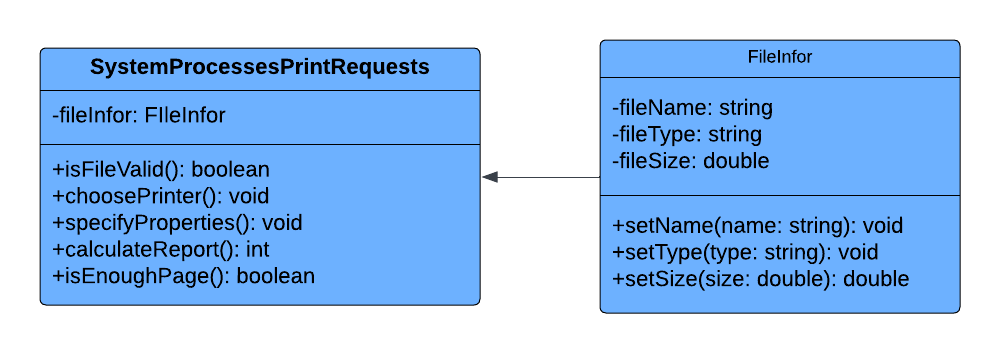
\includegraphics[scale=.9]{images/Task2/ClassDiagrams/RequestForPrintingService.png}
    \end{center}
    \label{refhinh1}
    \end{figure}
    \end{center}


    \subsubsection{Make Online Payment}
    \begin{center}
    \begin{figure}[!htp]
    \begin{center}
     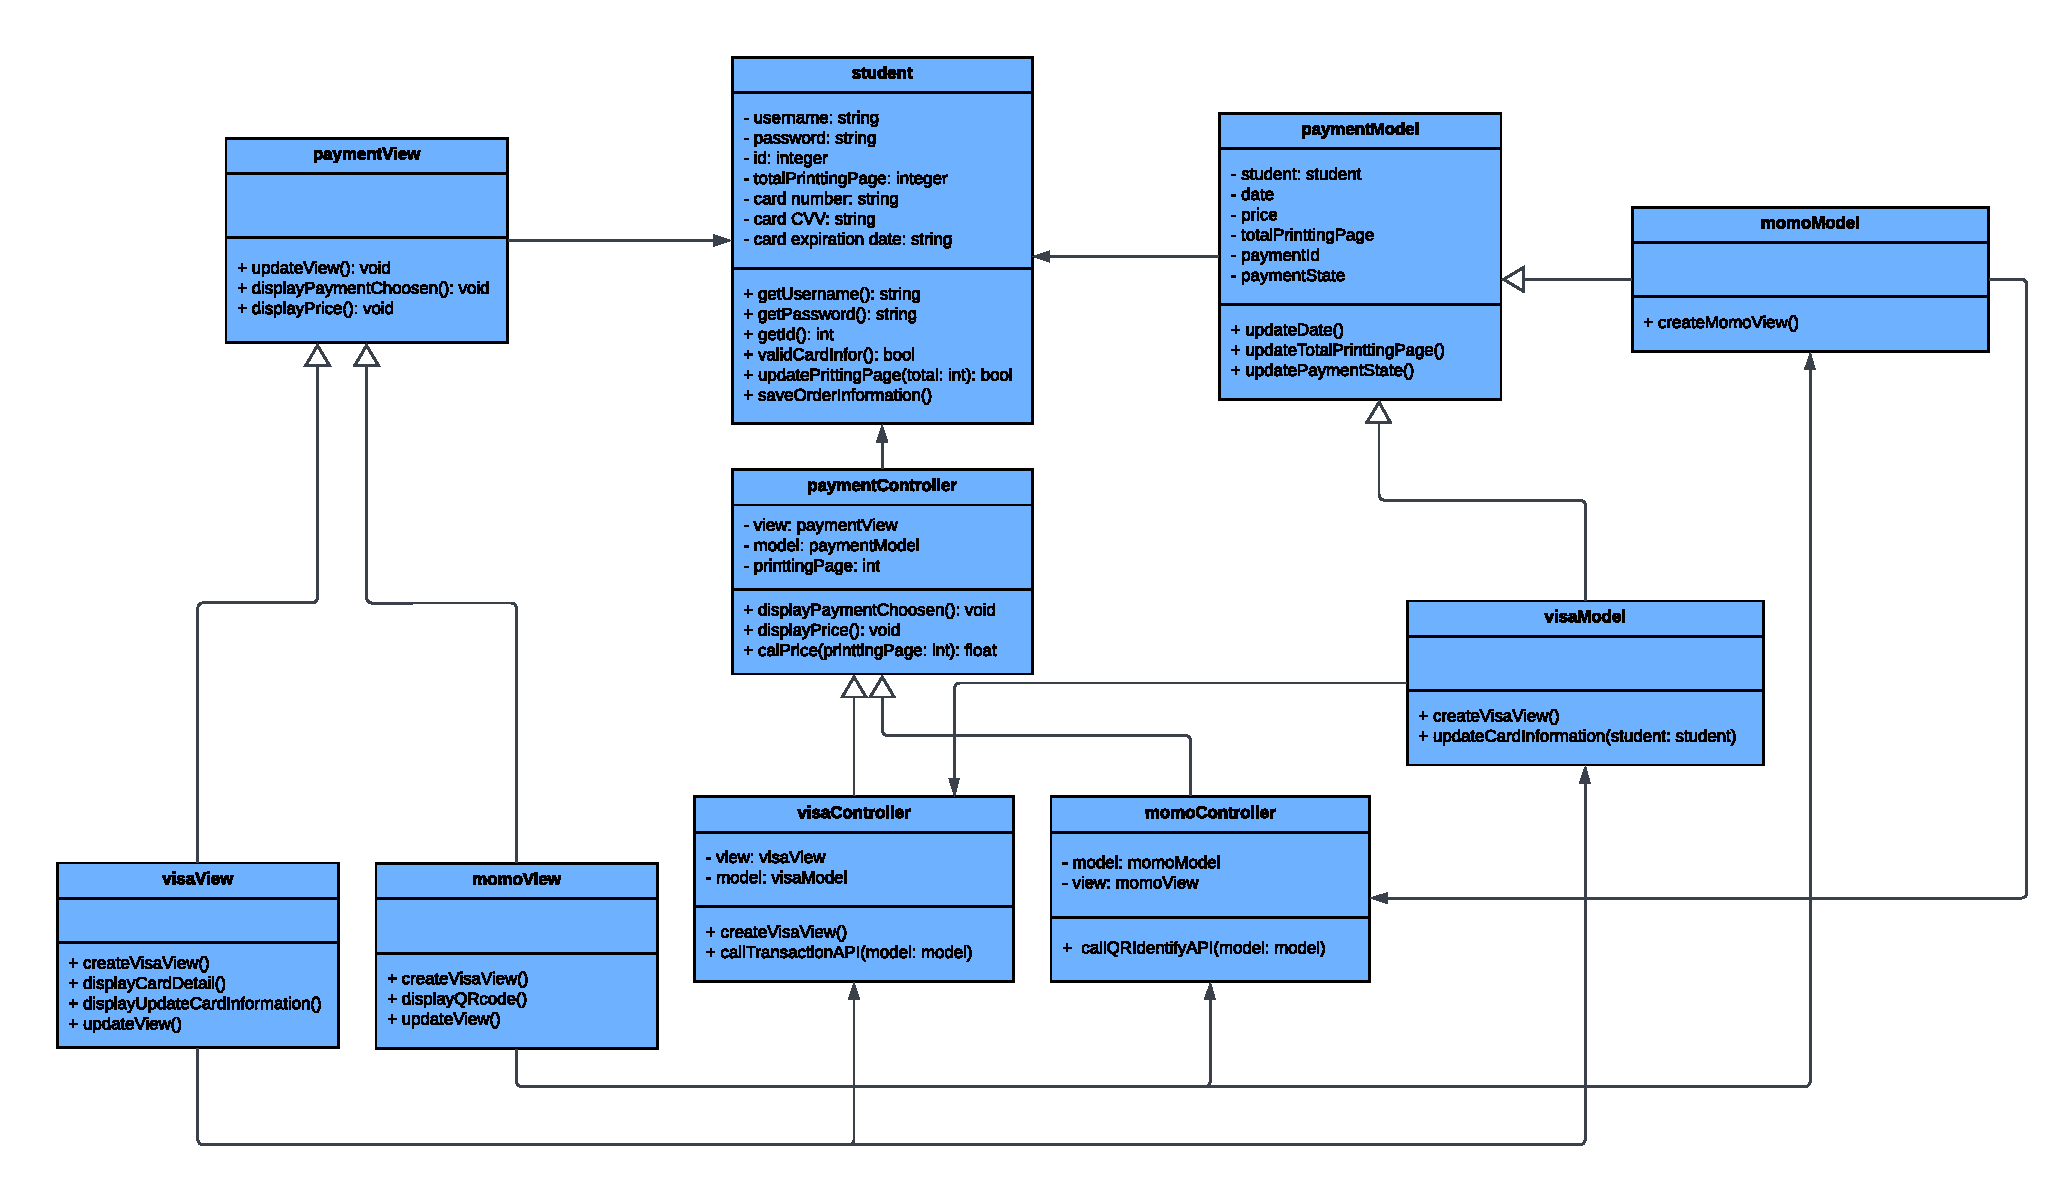
\includegraphics[scale=.5]{images/Task2/ClassDiagrams/PaymentClass.pdf}
    \end{center}
    \label{refhinh1}
    \end{figure}
    \end{center}



    \newpage
    \subsubsection{Manage Printers}
    \begin{center}
    \begin{figure}[!htp]
    \begin{center}
     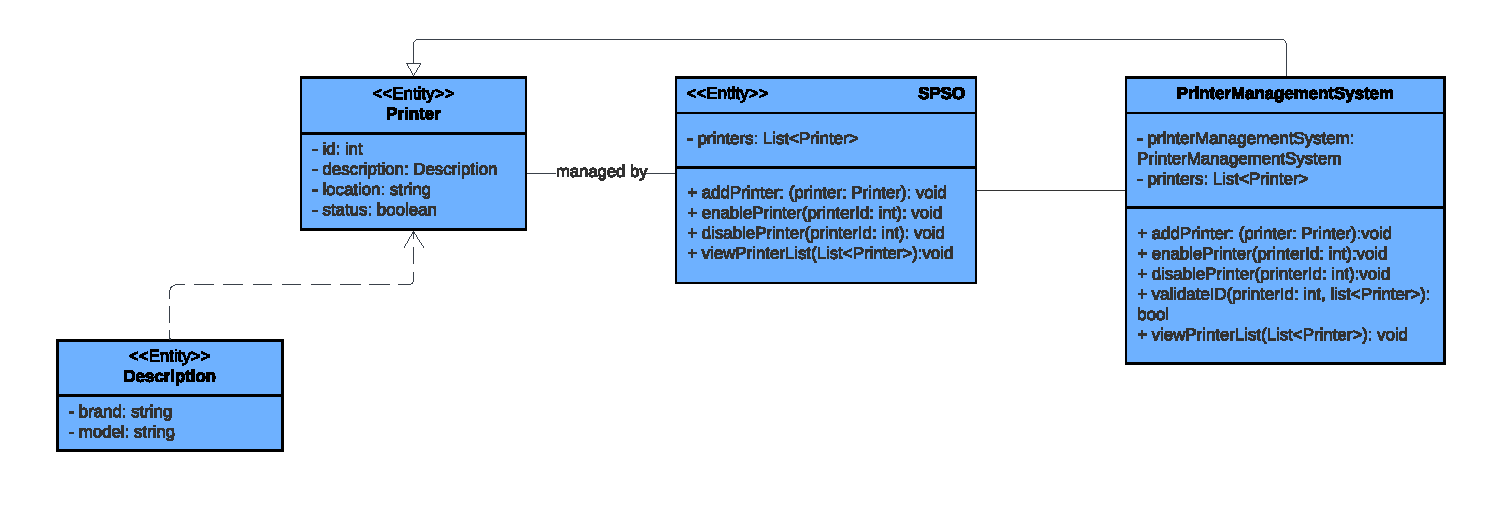
\includegraphics[scale=.5]{images/Task2/ClassDiagrams/ManagingPrinters.pdf}
    \end{center}
    \label{refhinh1}
    \end{figure}
    \end{center}


    \subsubsection{Configure System}
    \begin{center}
    \begin{figure}[!htp]
    \begin{center}
     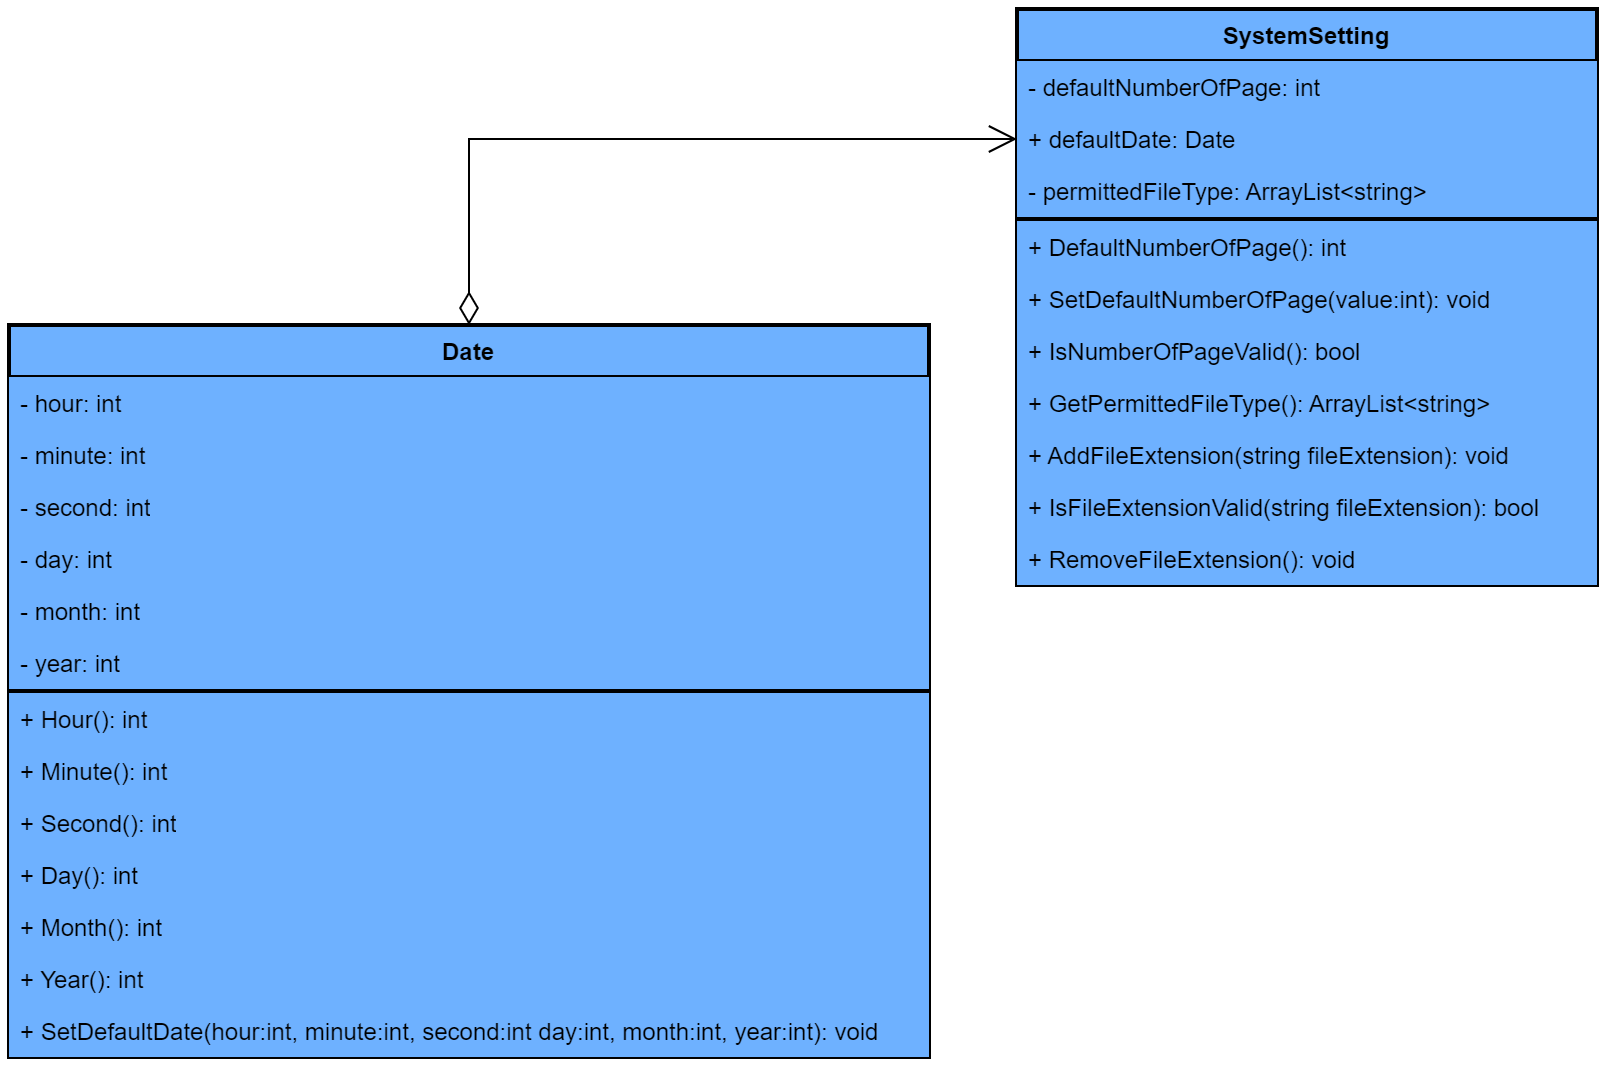
\includegraphics[scale=.2]{images/Task2/ClassDiagrams/ConfigureSystemClassDiagram.drawio (1).png}
    \end{center}
    \label{refhinh1}
    \end{figure}
    \end{center}


    \newpage
    \subsubsection{Log In}
    \begin{center}
    \begin{figure}[!htp]
    \begin{center}
     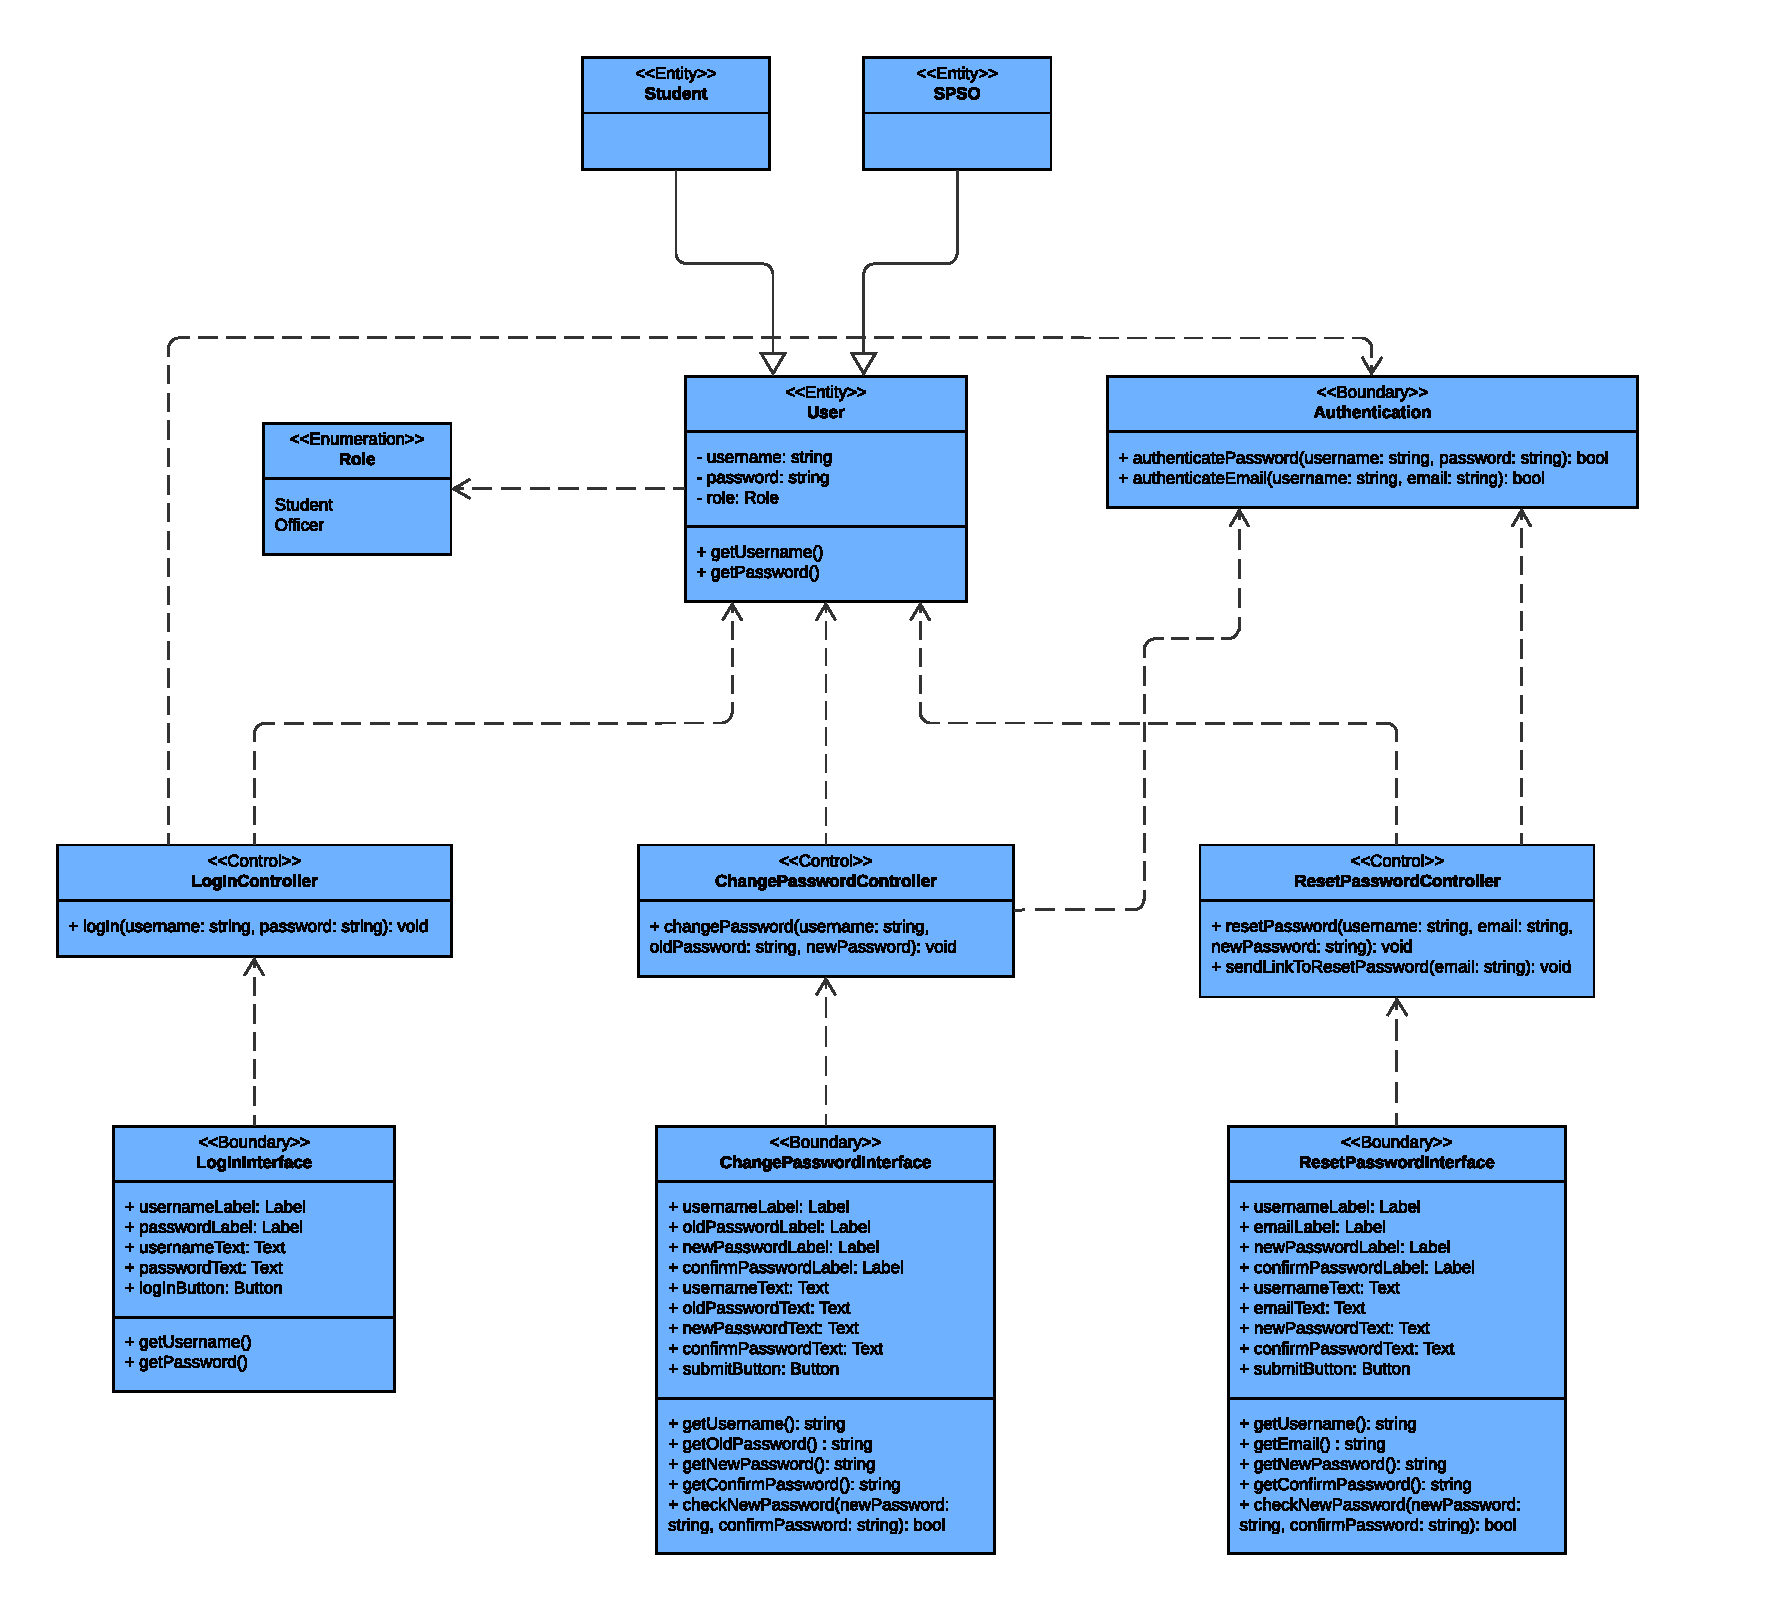
\includegraphics[scale=.5]{images/Task2/ClassDiagrams/LogIn.pdf}
    \end{center}
    \label{refhinh1}
    \end{figure}
    \end{center}

    \newpage
        \subsection{Task 2.4: Design User Interface}
    Liên kết đến thiết kế trong Figma: \href{https://www.figma.com/file/iKigk9Qx8GSMj3kLY0gqzQ/Nhom7_report_3?type=design&node-id=0%3A1&mode=design&t=Ja6DS4vqBqHGVIOn-1}{Nhom7\_report\_3}
    \subsubsection{Giao diện chung}
    \subsubsubsection{Giao diện trang chủ}
    \begin{center}
    \begin{figure}[!htp]
    \begin{center}
     \includegraphics[scale=.32]{images/Task 2.4/TrangChu.png}
    \end{center}
    \label{refhinh1}
    \end{figure}
    \end{center}
    \textbf{Mô tả:}
    \begin{itemize}
    \item Đây là giao diện đầu tiên khi người dùng truy cập vào trang web.
    \item Người dùng click vào "Đăng nhập" để tiến hành đăng nhập và sử dụng các dịch vụ.
    \end{itemize}

    \newpage
    \subsubsubsection{Giao diện đăng nhập}
    \begin{center}
    \begin{figure}[!htp]
    \begin{center}
     \includegraphics[scale=.32]{images/Task 2.4/DangNhap.png}
    \end{center}
    \label{refhinh1}
    \end{figure}
    \end{center}

    \textbf{Mô tả:}
    \begin{itemize}
        \item Giao diện bao gồm khu vực nhập thông tin đăng nhập (tài khoản, mật khẩu) của người dùng và một số thông tin như lưu ý, thông tin hỗ trợ kỹ thuật và bản quyền.
        \item Khu vực nhập thông tin bao gồm khung nhập thông tin tài khoản, mật khẩu, nút chọn đăng nhập và nút xóa thông tin đã nhập bên trên. Ngoài ra còn có checkbox để người dùng chọn cảnh báo khi có người đăng nhập vào trang web khác.
        \item Bên cạnh đó, khi người dùng muốn thay đổi mật khẩu hay họ quên mật khẩu và cần lấy lại thì có thể chọn để chuyển hướng đến trang đổi mật khẩu và quên mật khẩu.
    \end{itemize}
    \newpage
    \subsubsubsection{Giao diện thay đổi mật khẩu}
    \begin{center}
    \begin{figure}[!htp]
    \begin{center}
     \includegraphics[scale=.32]{images/Task 2.4/ChangePassword.png}
    \end{center}
    \label{refhinh1}
    \end{figure}
    \end{center}
    
    \textbf{Mô tả:}
    \begin{itemize}
        \item Giao diện bao gồm khu vực nhập thông tin để thay đổi mật khẩu bao gồm username, old password, new password và confirm new password.
        \item Sau khi bấm chọn submit thì hệ thống sẽ xác nhận thông tin và thay đổi mật khẩu cho người dùng. Nếu thông tin sai thì sẽ hiển thị thông báo để người dùng nhập lại.
        \item Bên cạnh đó, ở phần đầu trang còn có khu vực để người dùng có thể chuyển sang giao diện đặt lại mật khẩu.
    \end{itemize}
    \newpage
    \subsubsubsection{Giao diện đặt lại mật khẩu}
    \begin{center}
    \begin{figure}[!htp]
    \begin{center}
     \includegraphics[scale=.32]{images/Task 2.4/ResetPassword.png}
    \end{center}
    \label{refhinh1}
    \end{figure}
    \end{center}

    \textbf{Mô tả:}
    \begin{itemize}
        \item Giao diện bao gồm khu vực nhập thông tin để đặt lại mật khẩu bao gồm username, và email.
        \item Sau khi bấm chọn submit thì hệ thống sẽ xác nhận thông tin và gửi "link" xác thực việc đặt lại mật khẩu thông qua email mà người dùng cung cấp. Người dùng cần truy cập vào "link" này và hoàn thành các bước tiếp theo để đặt lại mật khẩu.
        \item Bên cạnh đó, ở phần đầu trang còn có khu vực để người dùng có thể chuyển sang giao diện thay đổi mật khẩu.
    \end{itemize}
    \newpage
    \subsubsection{Giao diện của sinh viên}
    \subsubsubsection{Giao diện dịch vụ của tôi}
    \begin{center}
    \begin{figure}[!htp]
    \begin{center}
     \includegraphics[scale=.32]{images/Task 2.4/DichVuCuaToi(SV).png}
    \end{center}
    \label{refhinh1}
    \end{figure}
    \end{center}

    \textbf{Mô tả:}
    \begin{itemize}
    \item Khi người dùng click chọn vào "DỊCH VỤ CỦA TÔI", danh sách các dịch vụ của từng đối tượng sẽ được hiển thị tại đây.
    \item Nếu là sinh viên, danh sách dịch vụ sẽ gồm: ĐĂNG KÍ IN TÀI LIỆU, MUA THÊM TRANG IN, NHẬT KÍ SỬ DỤNG DỊCH VỤ IN.
    \end{itemize}
    
    \newpage
    \subsubsubsection{Giao diện đăng kí in tài liệu}
    \begin{center}
    \begin{figure}[!htp]
    \begin{center}
     \includegraphics[scale=.32]{images/Task 2.4/DangKiIn.png}
    \end{center}
    \label{refhinh1}
    \end{figure}
    \end{center}
    \textbf{Mô tả:}
    \begin{itemize}
        \item Giao diện bao gồm chọn tập tin, tùy chọn thuộc tính, chọn máy in và nút xác nhận đăng ký.
        \item Sinh viên chỉ được tải lên một file duy nhất, hệ thống sẽ tự động kiểm tra tính hợp lệ của file và thông báo lại cho sinh viên.
        \item Nút "Tùy chọn thuộc tính" chỉ khả dụng sau khi file hợp lệ được tải lên, sinh viên có thể chọn máy in trước khi tải file.
        \item Sinh viên có thể không cần tùy chọn thuộc tính và các thuộc tính sẽ được đặt mặc định.
        \item Sau Khi file hợp lệ được tải lên và máy in được chọn sinh viên phải nhấn nút "Đăng ký" để tiến hành in. Nút "Đăng ký" sẽ không khả dụng cho tới sinh viên thực hiện đủ hai điều kiện nêu trên.
    \end{itemize}
    \newpage
    \subsubsubsection{Giao diện tuỳ chọn thuộc tính in}
    \begin{center}
    \begin{figure}[!htp]
    \begin{center}
     \includegraphics[scale=.32]{images/Task 2.4/TuyChonThuocTinh.png}
    \end{center}
    \label{refhinh1}
    \end{figure}
    \end{center}
    \textbf{Mô tả:}
    \begin{itemize}
        \item Giao diện bao gồm các thuộc tính như khổ giấy, trang in, mặt in và số lượng in. Ngoài ra còn có phần preview các trang ở bên trái để sinh viên có cái nhìn tổng quát.
        \item Tất cả các thuộc tính đều được đặt mặc định sẵn như trong hình.
        \item Sau khi cài đặt các thuộc tính xong sinh viên cần nhấn nút "Hoàn tất" để lưu lại cài đặt.
        \item Nút "Đặt về mặc định" cấu hình lại các thuộc tính về mặc định đề phòng trường hợp sinh viên chỉnh các thuộc tính không ưng ý. 
    \end{itemize}
    
    \newpage
    \subsubsubsection{Giao diện mua trang in}
    \begin{center}
    \begin{figure}[!htp]
    \begin{center}
     \includegraphics[scale=.32]{images/Task 2.4/MuaTrangIn.png}
    \end{center}
    \label{refhinh1}
    \end{figure}
    \end{center}

    \textbf{Mô tả:}
    \begin{itemize}
    \item Hệ thống cung cấp thông tin về số trang in hiện tại của người dùng (theo khổ A4).
    \item Khi muốn mua thêm trang trang in, sinh viên nhập số lượng cần mua và bấm nút "Đăng ký" để tạo đơn hàng.
    \item Trường "Lịch sử đăng ký" sẽ cung cấp thông tin về tất cả các đăng ký mua trang in của sinh viên. Ở cột "Thanh toán", có 2 giá trị là "Đã thanh toán" và "Thanh toán ngay" (nếu sinh viên chưa thanh toán).
    \end{itemize}

    \newpage
    \subsubsubsection{Giao diện chọn hình thức thanh toán}
    \begin{center}
    \begin{figure}[!htp]
    \begin{center}
     \includegraphics[scale=.32]{images/Task 2.4/ThanhToan.png}
    \end{center}
    \label{refhinh1}
    \end{figure}
    \end{center}

    \textbf{Mô tả:}
    \begin{itemize}
    \item Từ giao diện mua trang in, để thanh toán đơn hàng, sinh viên click vào "Thanh toán ngay".
    \item Khi đó, một của sổ "Chọn hình thức thanh toán" sẽ bật lên. Sinh viên cần lựa chọn hình thức thanh toán phù hợp.
    \begin{itemize}
        \item Sinh viên có thể chọn "Quay lại" nếu không muốn thực hiện thanh toán.
        \item Khi sinh viên nhấn "Tiếp tục" thì trang web sẽ chuyển sang trang cổng thanh toán của các bên dịch vụ tương ứng. Tại đó, sinh viên sẽ tiếp tục các bước thanh toán theo yêu cầu của cổng thanh toán.
    \end{itemize}
    \item Sau khi hoàn tất thanh toán, giao diện sẽ cập nhật trang thái từ "Thanh toán ngay" thành "Đã thanh toán" và "Số trang in hiện tại" cũng sẽ được cập nhật.
    \end{itemize}


    \newpage
    \subsubsection{Giao diện của SPSO}
    \subsubsubsection{Giao diện dịch vụ của tôi}
    \begin{center}
    \begin{figure}[!htp]
    \begin{center}
     \includegraphics[scale=.32]{images/Task 2.4/DichVuCuaToi(SPSO).png}
    \end{center}
    \label{refhinh1}
    \end{figure}
    \end{center}

    \textbf{Mô tả:}
    \begin{itemize}
    \item Khi người dùng click chọn vào "DỊCH VỤ CỦA TÔI", danh sách các dịch vụ của từng đối tượng sẽ được hiển thị tại đây.
    \item Nếu là SPSO, danh sách dịch vụ sẽ gồm: QUẢN LÝ CÁC MÁY IN, CẤU HÌNH HỆ THỐNG, NHẬT KÍ SỬ DỤNG DỊCH VỤ IN CỦA SINH VIÊN, CÁC BÁO CÁO VỀ VIỆC SỬ DỤNG DỊCH VỤ IN.
    \end{itemize}

    \newpage
    \subsubsubsection{Giao diện thêm máy in mới}
    \begin{center}
    \begin{figure}[!htp]
    \begin{center}
     \includegraphics[scale=.32]{images/Task 2.4/ThemMayIn.png}
    \end{center}
    \label{refhinh1}
    \end{figure}
    \end{center}

    \textbf{Mô tả:}
    SPSO sẽ chọn cơ sở đào tạo và tòa nhà cần lắp đặt thêm máy in. Sau đó, SPSO sẽ nhập ID cho máy in mới
    \begin{itemize}
        \item Nếu ID hợp lệ thì ID sẽ chuyển sang màu xanh và SPSO có thể tiếp tục nhập Tên, Mẫu mã và các ghi chú đính kèm. Sau đó, SPSO có thể nhấn xác nhận để thêm máy in vào hệ thống.
        \item Nếu ID không hợp lệ, ID sẽ chuyển sang màu đỏ và SPSO sẽ cần phải nhập lại ID
    \end{itemize} 
    
    \newpage
    \subsubsubsection{Giao diện quản lí máy in}
    \begin{center}
    \begin{figure}[!htp]
    \begin{center}
     \includegraphics[scale=.32]{images/Task 2.4/QuanLyMayIn.png}
    \end{center}
    \label{refhinh1}
    \end{figure}
    \end{center}

    \textbf{Mô tả:}
    SPSO có thể lựa chọn cơ sở đào tạo, tòa nhà và máy in cụ thể để hiện ra các thông tin hiện tại của máy in đó. Nếu muốn thay đổi trạng thái hoạt động của máy in đó, SPSO có thể nhấn vào nút (Thay đổi) để hiện lên pop-up. Khi đó, pop-up sẽ yêu cầu SPSO nhập ID để xác nhận sau đó chọn bật hoặc tắt theo nhu cầu.

    \newpage
    \subsubsubsection{Giao diện cấu hình hệ thống}
    \begin{center}
    \begin{figure}[!htp]
    \begin{center}
     \includegraphics[scale=.32]{images/Task 2.4/CauHinhHeThong.png}
    \end{center}
    \label{refhinh1}
    \end{figure}
    \end{center}

    \textbf{Mô tả:}
    Theo như các diagram trước đó về configure system, 3 chức năng chính được chia theo 3 nhánh hoạt động riêng. Tuy nhiên trong quá trình thiết kế và hiện thực, việc chia chức năng ra như vậy là không cần thiết và tương đối lãng phí không gian trong giao diện. Vì vậy, một quyết định được đưa ra đó là gộp 3 chức năng đó vào trong 1 trang duy nhất. Khi nhấn lưu thì tất cả thông số mặc định sẽ đồng thời được kiểm tra và cập nhật.\\

	%%%%%%%%%%%%%%%%%%%%%%%%%%%%%%%%%
        \newpage
	\section{Task 3: Architecture design}
        \subsection{Deployment Diagrams}
        \begin{center}
        \begin{figure}[!htp]
        \begin{center}
         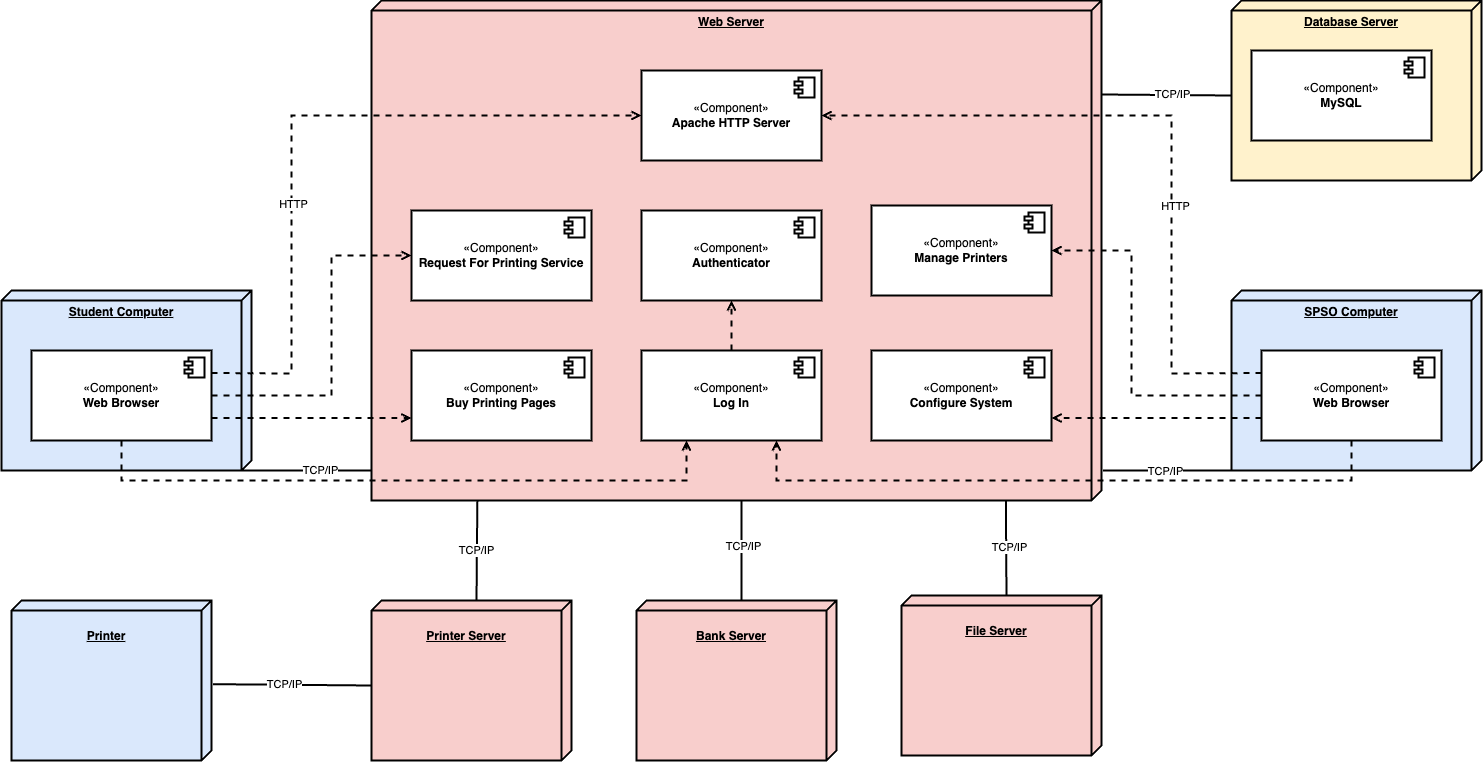
\includegraphics[scale=0.3]{images/Task3/Deployment Diagram/DeploymentDiagram(v1).drawio.png}
        \end{center}
        \end{figure}
        \end{center}

        \textbf{Mô tả:}
        \begin{itemize}
            \item Người dùng (sinh viên, người quản lí) sẽ  kết nối tới Web Server bằng Web Browser qua giao thức TCP/IP.
            \item Web Server sẽ cung cấp các dịch vụ và giao diện cho sinh viên và nhân viên quản lí:
            \begin{itemize}
                \item Dịch vụ sinh viên: Tính năng chính: đăng nhập (bao gồn Login, Change Password, Reset Password), tạo yêu cầu in (Request for printing service), mua thêm trang in (Buy Printing Pages) và thanh toán khi mua trang in (Online Payment). Ngoài ra còn có các tính năng phụ như: sinh viên có thể xem nhật kí sử dụng dịch vụ in của mình.
                \item Dịch vụ nhân viên quản lí: đăng nhập (Login, ChangePassword, Reset Password), quản lí các máy in (Manage Printers), cấu hình hệ thống (Configure System). Ngoài ra còn có một số tính năng phụ như: xem nhật kí sử dụng dịch vụ in của sinh viên, xem báo cáo thông kê về sử dụng dịch vụ in hằng tháng của hệ thống.
            \end{itemize}
            \item Web Server sẽ giao tiếp với Database Server qua qua giao thức TCP/IP.
            \item Database Server sử dụng mySQL và chứa các dữ liệu về sinh viên (student), nhân viên (SPSO), máy in (printer), tập tin (file), yêu cầu in (print request), thanh toán (payment), cấu hình hệ thống (configuration) v.v. Website sẽ tương tác với dữ liệu này thông qua REST API.
            \begin{itemize}
                \item REST sử dụng các yêu cầu HTTP như GET, PUT, POST và DELETE để quản lý các hoạt động CRUD (Create, Read, Update, and Delete).
                \item Dữ liệu được trả về với định dạng JSON.
            \end{itemize}
            
        \end{itemize}
        \newpage
	\subsection{Component Diagrams}
        \subsubsection{Request For Printing Service}
        \begin{center}
        \begin{figure}[!htp]
        \begin{center}
         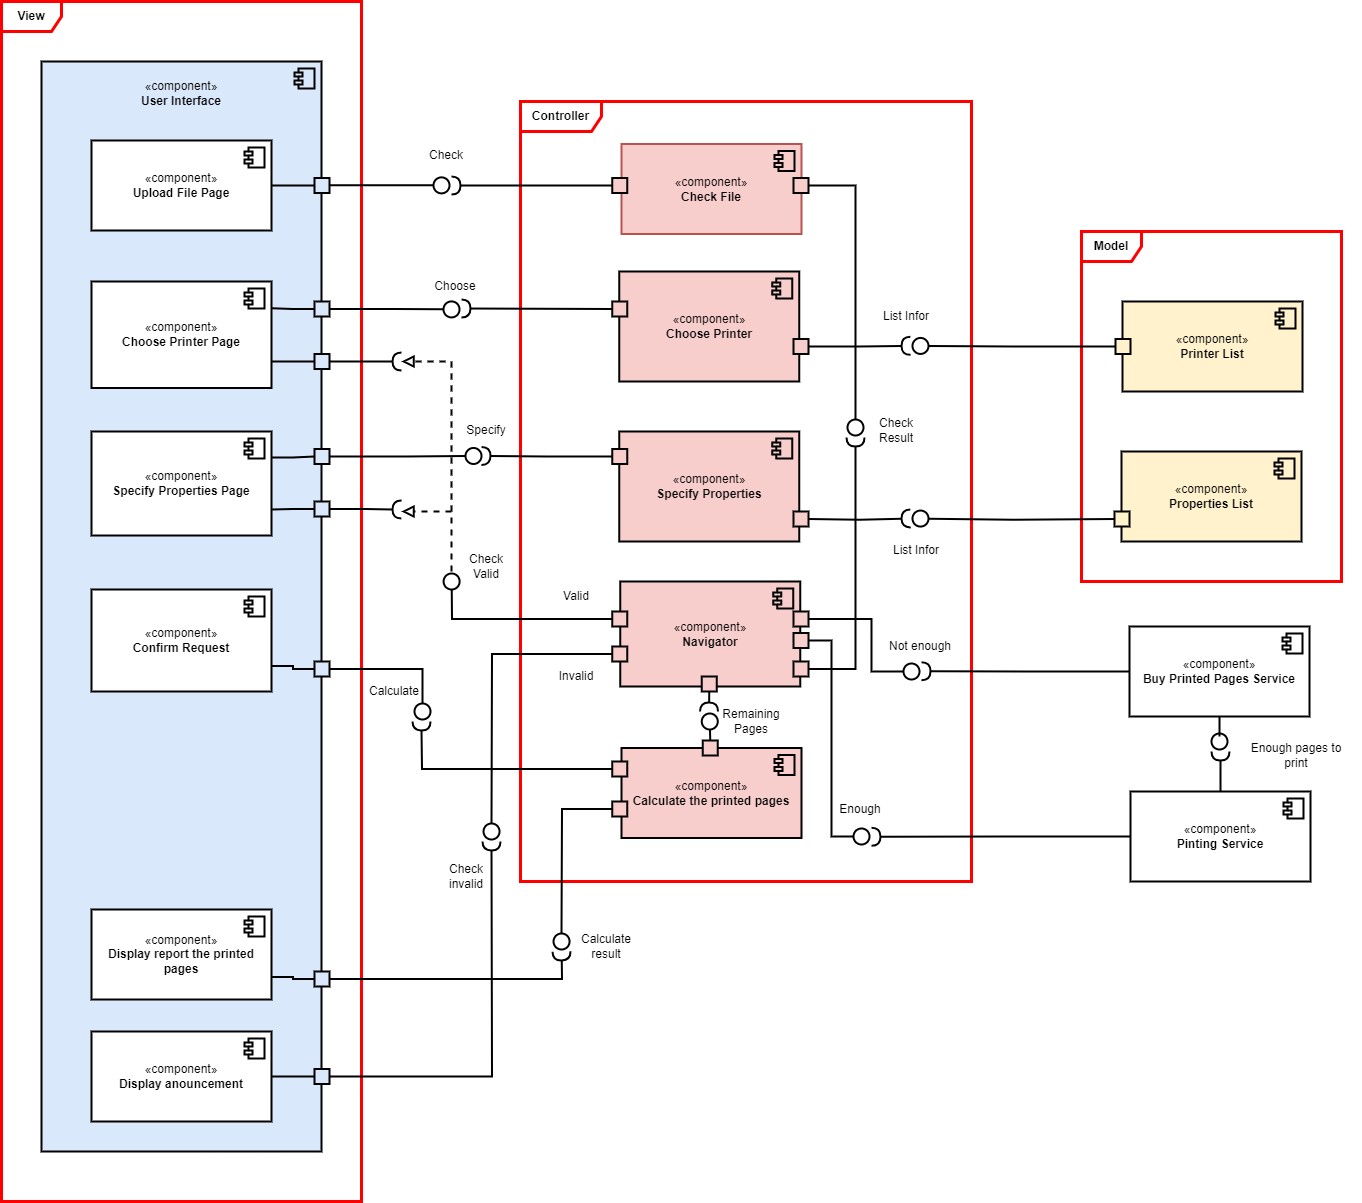
\includegraphics[scale=0.31]{images/Task3/Component Diagrams/RequestForPrintingService.png}
        \end{center}
        \end{figure}
        \end{center}

        \newpage
        \textbf{Mô tả:}
        \begin{itemize}
            \item File khi được tải lên hệ thống sẽ được khối \textit{Check File} kiểm tra và gửi thông tin đến khối \textit{Navigator} để phân chia luồng xử lý:
            \begin{itemize}
                \item Nếu file không hợp lệ, \textit{Display anouncement} sẽ thông báo đến người dùng.
                \item Nếu file hợp lệ \textit{Choose Printer Page} và \textit{Specify Properties Page} sẽ được kích hoạt cho phép người dùng sử dụng.
            \end{itemize}
            \item \textit{Choose Printer Page} và \textit{Specify Properties Page} khi được kích hoạt bởi người dùng sẽ được xử lý lần lượt bởi các khối \textit{Choose Printer} và \textit{Specify Propertries}. Hai khối trên dựa vào yêu cầu của người dùng và thông tin trong \textit{Printer List}, \textit{Properties List} để xử lý.
            \item Sau khi hoàn tất các thao tác trên người dùng sẽ phải xác nhận yêu cầu \textit{Confirm Request} để tiếp tục, khối \textit{Calculate the printed pages} sẽ tính toán và gửi báo cáo đến người dùng xem họ còn lại bao nhiêu trang có thể in đồng thởi gửi tín hiệu đến khối \textit{Navigator}:
            \begin{itemize}
                \item Nếu số trang còn lại đủ để in tài liệu, \textit{Printing Service} sẽ kết nối với máy in và tiến hành in hoàn tất quá trình.
                \item Nếu số trang không đủ người dùng được chuyển đến chức năng \textit{Buy Printed Pages Service} để mua thêm trang in. Sau khi mua đủ số trang in cần thiết người dùng sẽ được chuyển đến \textit{Printing Service}để hoàn tất.
            \end{itemize}
        \end{itemize}

        \newpage
        \subsubsection{Make Online Payment}
        \begin{center}
        \begin{figure}[!htp]
        \begin{center}
         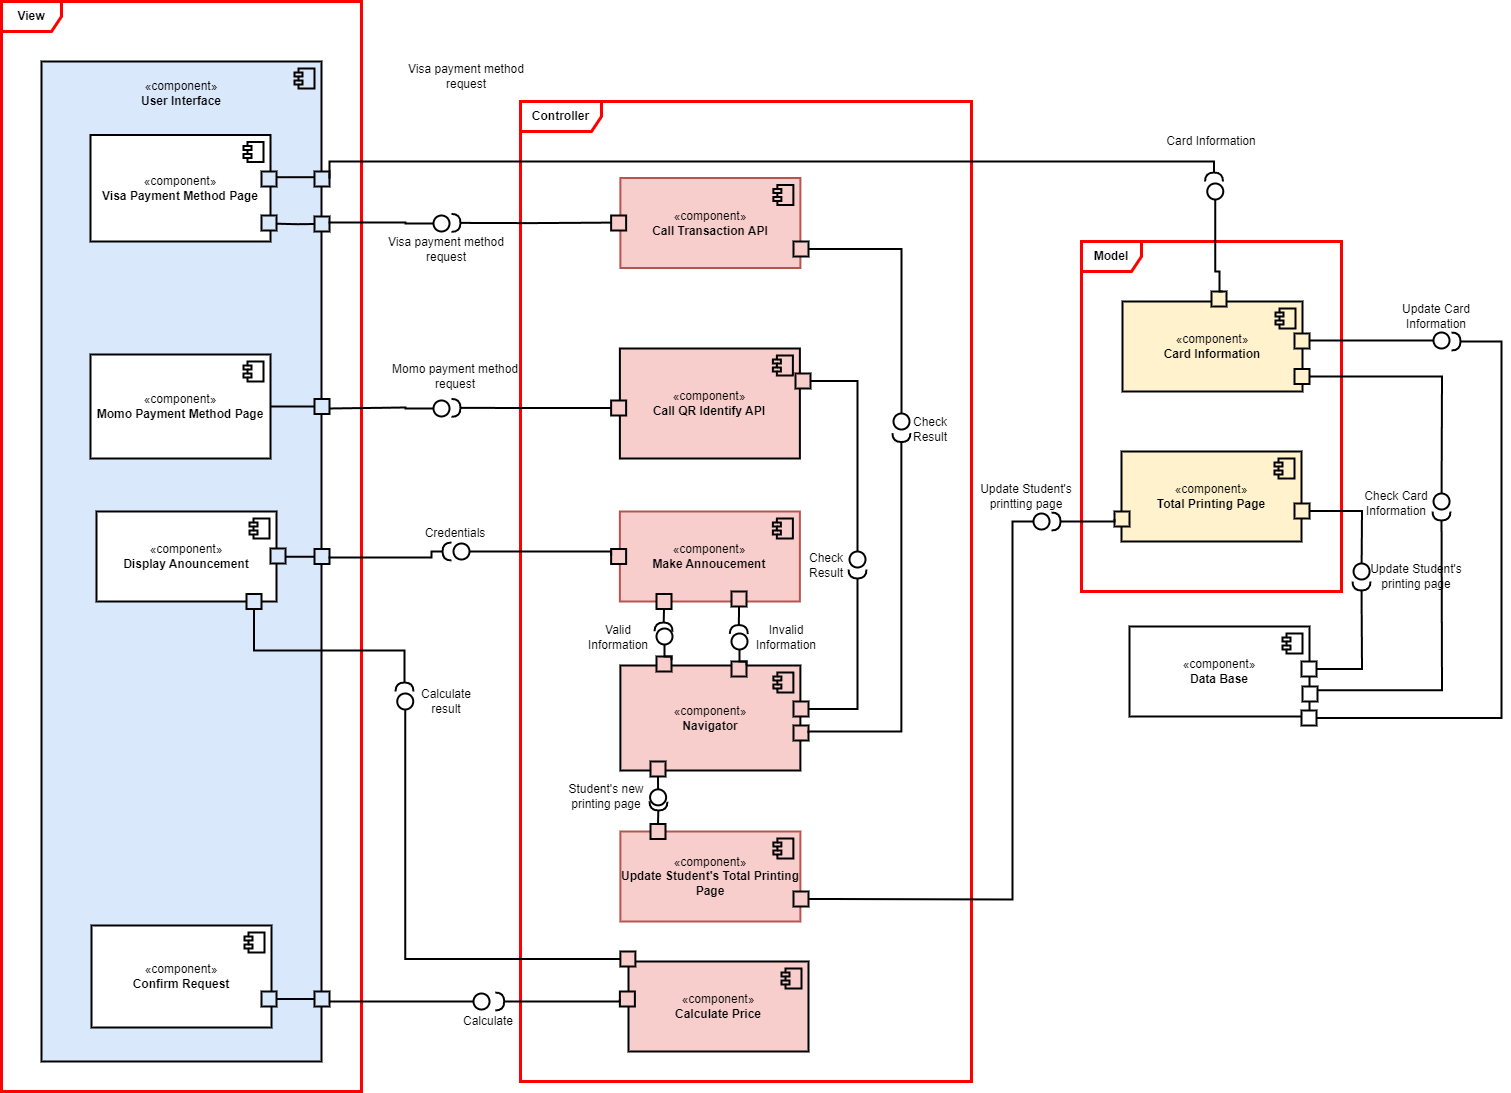
\includegraphics[scale=0.32]{images/Task3/Component Diagrams/paymentComponentDiagram.drawio.png}
        \end{center}
        \end{figure}
        \end{center}
        \newpage
        \textbf{Mô tả:}
        \begin{itemize}
            \item Tại giao diện \textit{Confirm Request} khi người dùng chọn số lượng trang in và đồng ý thì khối \textit{Calculate Price} sẽ thực hiện tính toán giá tiền và hiển thị cho người dùng thông qua khối \textit{Display Anouncement}. Đồng thời cũng tại giao diện này người dùng sẽ chọn phương thức thanh toán.
            \item Tại giao diện \textit{Visa Payment Method}, nếu thông tin về visacard của người dùng được đối chiếu qua khối \textit{Card Information} và \textit{Data Base} là hợp lệ thì thông tin thẻ sẽ được khối \textit{Call Transaction API} xử lí và thực hiện thanh toán. Còn nếu thông tin về thẻ không tồn tại thì người dùng sẽ nhập thông tin về thẻ trong giao diện \textit{Visa Payment Method} và khối \textit{Card Information} sẽ gửi yêu cầu Update Card Information đến khối \textit{Data Base}. Sau đó thông tin sẽ được khối \textit{Call Transaction API} xử lí và thực hiện thanh toán.
            \item Tại giao diện \textit{Momo Payment Method}, người dùng sẽ quét mã QR và thông tin này sẽ được khối \textit{Call QR Identify API} xử lí và thực hiện thanh toán.
            \begin{itemize}
                \item Trường hợp thông tin thanh toán chính xác: khối \textit{Navigator} sẽ tiến hành gửi số lượng trang in mới của sinh viên đến khối \textit{Update Student's Total Printting Page } và khối này sẽ gửi yêu cầu đến khối \textit{Total Printting Page} trong Model và cập nhật thông tin trong database.
                \item Trường hợp thông tin xác thực không chính xác: Người dùng có thể tiến hành nhập lại thông tin về thẻ thông qua giao diện \textit{Visa Payment Method} (trong trường hợp thanh toán qua visacard), quét lại mã QR qua giao diện \textit{Momo Payment Method} (trong trường hợp thanh toán qua momo) hoặc thoát khỏi qua trình mua trang in.    
            \end{itemize}
        \end{itemize}


        \newpage
        \subsubsection{Manage Printers}
        \begin{center}
        \begin{figure}[!htp]
        \begin{center}
         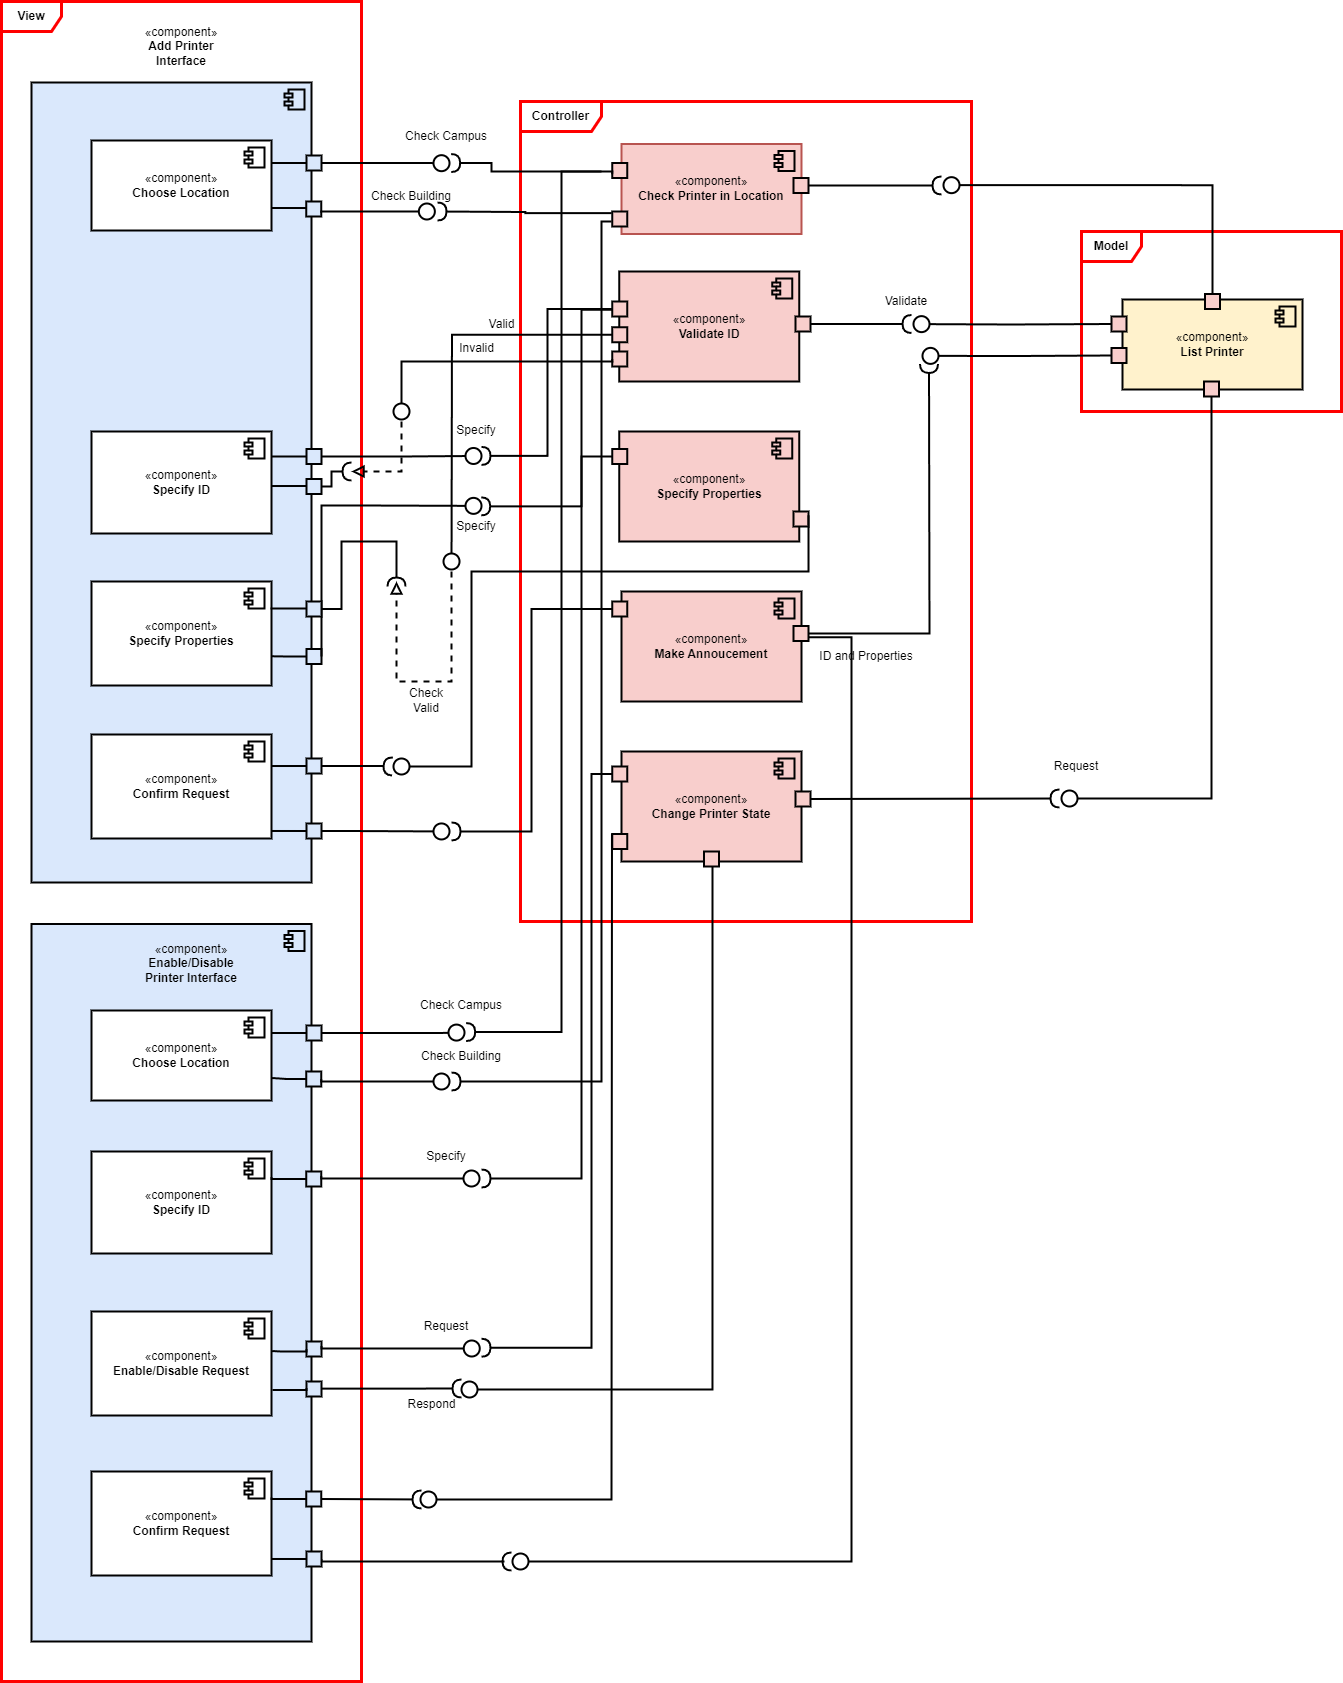
\includegraphics[scale=0.31]{images/Task3/Component Diagrams/ManagePrinterComponentDiagram.png}
        \end{center}
        \end{figure}
        \end{center}

        \newpage
        \textbf{Mô tả:}
        \begin{itemize}
            \item Tại giao diện \textit{Add Printers}, SPSO sẽ chọn cơ sở (campus) và tòa nhà (building) có sẵn, sau đó sẽ nhập ID của máy in mới muốn thêm vào hệ thống. ID đó sẽ đi qua khối \textit{Validate ID} để kiểm tra, nếu hợp lệ sẽ hiển thị hợp lệ và SPSO sẽ tiếp tục nhập các thông tin khác của máy in. Nếu không hợp lệ, tín hiệu sẽ được gửi đến khối \textit{Make Annoucement}, khối trả về thông báo ID không hợp lệ và SPSO sẽ phải nhập lại. Sau khi đã hoàn tất nhập các thông tin, SPSO sẽ nhấn Xác nhận và lưu thông tin vào Hệ thống các máy in.
            \item Tại giao diện \textit{Enable/Disable Printer}, SPSO sẽ chọn cơ sở (campus) và tòa nhà (building) có sẵn, sau đó sẽ nhập ID của máy in muốn thay đổi trạng thái. Nếu ID hợp lệ, khối \textit{Make Annoucement} trả về thông báo hợp lệ, SPSO có thể thay đổi trạng thái của máy in như mong muốn. Nếu không hợp lệ, tín hiệu sẽ được gửi đến khối \textit{Make Annoucement}, khối trả về thông báo ID không hợp lệ và SPSO sẽ phải nhập lại. Sau khi đã xác nhận trạng thái, SPSO có thể xác nhận thay đổi và khối \textit{Change Printer State} sẽ thay đổi trạng thái của máy in.
        \end{itemize}



        \newpage
        \subsubsection{Configure System}
        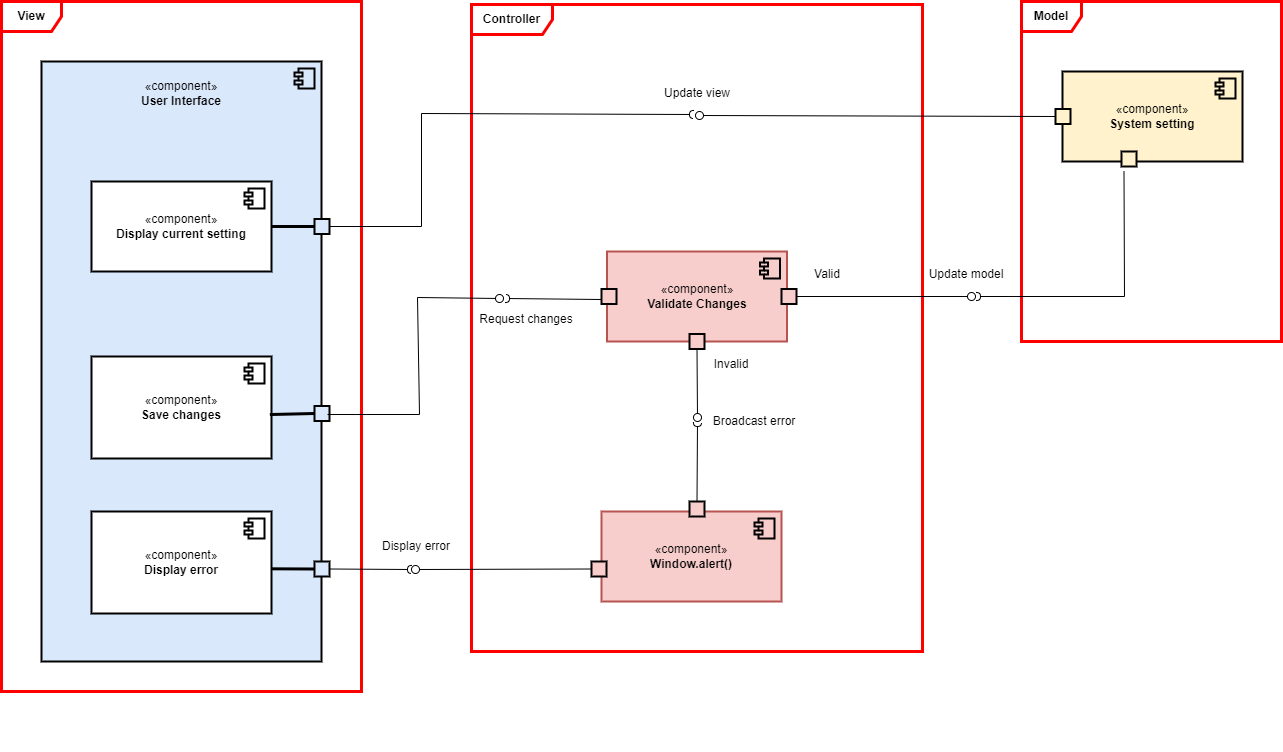
\includegraphics[width=\textwidth]{images/Task3/Component Diagrams/ConfigureSystemComponentDiagram.drawio.png}
        \textbf{Mô tả:}
        Thao tác thay đổi các thiết lập của hệ thống bao gồm các component chính là Display current setting ở phần view, Validate changes ở phần Controller và System setting ở phần model.
        \begin{itemize}
            \item Khi vào trang thay đổi các thiết lập của hệ thống, System setting sẽ cập nhật các thông tin hiển thị cho người dùng bằng dữ liệu được lưu trong hệ thống.
            \item Nếu người dùng lưu thay đổi, Controller sẽ tiếp nhận việc kiểm tra dữ liệu được thay đổi.
            \item Nếu dữ liệu mới hợp lệ, controller sẽ tiến hành giao tiếp với model để cập nhật system setting và system setting sẽ cập nhật lại giao diện người dùng bằng dữ liệu mới.
            \item Nếu dữ liệu mới không hợp lệ, controller gọi hàm window.alert để báo lỗi lên giao diện người dùng.
        \end{itemize}

        \newpage
	\subsubsection{Log In}
        \begin{center}
        \begin{figure}[!htp]
        \begin{center}
         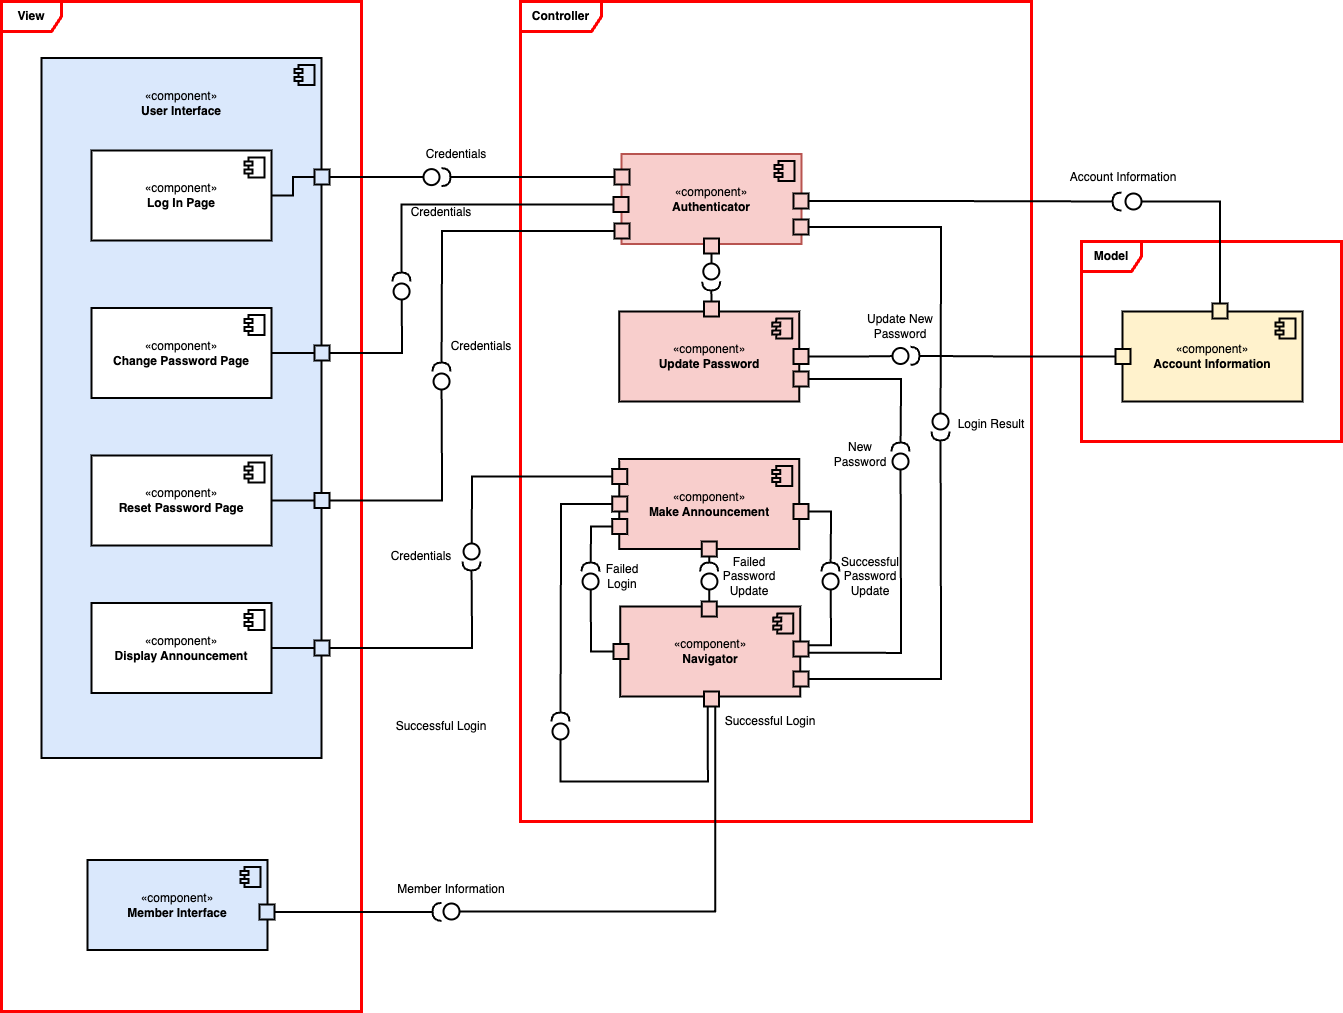
\includegraphics[scale=0.31]{images/Task3/Component Diagrams/ComponentDiagramLogin.drawio.png}
        \end{center}
        \end{figure}
        \end{center}

        \newpage
	\textbf{Mô tả:}
        \begin{itemize}
            \item Tại giao diện đăng nhập \textit{(Login Page)}, người dùng cung cấp các thông tin xác thực theo yêu cầu \textit{(username, password)}. Thông tin này sẽ được khối \textit{Authenticator} tiếp nhận và đối chiếu với dữ liệu từ \textit{Account Information} trong model. Sau đó kết quả được gửi đến khối \textit{Navigator} để tiến hành điều hướng, đồng thời thông báo đến cho người dùng qua khối \textit{Display Announcement}.
            \begin{itemize}
                \item Trường hợp thông tin đăng nhập chính xác: Người dùng sẽ được điều hướng đến giao
                diện dành cho thành viên với các thông tin của tài khoản đó..
                \item Trường hợp thông tin xác thực không chính xác: Người dùng có thể tiến hành đăng nhập lại hoặc chọn đặt lại mật khẩu (\textit{Reset password}).    
            \end{itemize}
            \item Tương tự, tại giao diện thay đổi mật khẩu (\textit{Change Password}) và đặt lại mật khẩu (\textit{Reset Password}), người dùng cũng cần nhập các thông tin xác thực cần thiết (\textit{username, old password, new password, confirm password} đối với \textit{Change Password} và \textit{username, email, new password, confirm password} đối với \textit{Reset Password}). Khối \textit{Authenticator} sẽ tiếp nhận và tiến hành xác thực các thông tin này với dữ liệu từ \textit{Account Information}. Kết quả xác thực này sẽ được gửi đến khối \textit{Navigator} để tiến hành điều hướng thích hợp và thông báo đến người dùng qua khối \textit{Display Announcement}.
            \begin{itemize}
                \item Trường hợp thông tin đăng nhập chính xác: Khối \textit{Update Password} sẽ được kích hoặc và tiến hành cập nhật lại mật khẩu mới vào tài khoản người dùng.
                \item Trường hợp thông tin xác thực không chính xác: Người dùng cần tiến hành nhập thông tin xác thực lại.
            \end{itemize}
        \end{itemize}
        
        
        
        
        
        
 %%%%%%%%%%%%%%%%%%%%%%%%%%%%%%%%%%%%%%%%%%%%%%%%%%%%
    \newpage
	\section{Task 4: Implementation - Sprint 1}
	\input{task4}
	%%%%%%%%%%%%%%%%%%%%%%%%%%%%%%%%%%%%%%%%%%%%%%%%%%%%
	\section{Task 5: Implementation - Sprint 2}
	
	
	%%%%%%%%%%%%%%%%%%%%%%%%%%%%%%%%%%%%%%%%%%%%%%%%%%%%
	\newpage
	\addcontentsline{toc}{section}{\protect\numberline{}Tài liệu tham khảo}
	%\renewcommand\refname{Tài liệu tham khảo}
	\begin{thebibliography}{80}
		\bibitem{bib1}
		...
		\bibitem{bib2}
		...
	\end{thebibliography}
\end{document}

